\chapter{Maschinelles Lernen}

Im ersten Kapitel sollen die Grundlagen für ein fundiertes Verständnis
von Maschinellem Lernen gelegt werden. Neben den verschieden Arten sollen
essenzielle Begriffe und das Modellkonzept dargelegt werden. Darüber hinaus werden
die Funktionsweise des Trainings sowie daraus entstehende Phänomene erläutert.
Auf dieser Basis erfolgt in Kapitel zwei die Darlegung eines konkreten Modells.
\para{}
\bigskip
\keyword{Maschinellen Lernens} beschäftigt sich mit Algorithmen und
mathematischen Modellen, welche die Fähigkeit entwickeln, Probleme selbstständig
zu lösen.
Hierbei wird nicht explizit einprogrammiert, wie ein Modell das Problem zu lösen
hat, stattdessen wird das Modell trainiert, optimiert sich von selbst und findet allein
einen Weg, die Aufgabenstellung zu lösen.
Die Grundidee dabei ist, dass Daten erfasst, generiert oder gemessen werden,
welche anschliessend analysiert werden sollen.
Innerhalb dieser Daten existieren gewisse
Gesetzmässigkeiten und Muster. Diese Muster sollen vom Modell
erkannt und verallgemeinert werden. Nach dem erfolgreichen Lernprozess
kann das Modell Vorhersagen für neue Daten machen.
\para{}
Wir unterscheiden zwei Arten von Maschinellem Lernen%
\footnote{
  Es existieren noch weitere Arten von ML, wie zum Beispiel
  \keyword{Semi-Supervised Learning} und
  \keyword{Reinforcement Learning}. Für diese Arbeit sind diese aber nicht
  weiter relevant.
}:
\begin{itemize}
\item{
    \keyword{Überwachtes Lernen} (engl.:\ supervised learning) ist ein
    Lernverfahren, bei welchem die Daten aus zwei Teilen bestehen, aus Inputs und
    Outputs. Man bezeichnet dabei die Outputs als Labels. Die Aufgabe des Modells
    ist es, eine \keyword{Korrelation} zwischen den Inputs und den Labels zu
    erlernen und so ihre Beziehung zueinander zu verstehen.
    Anhand der Informationen, welche die Inputs enthalten,
    können die Labels vorhergesagt werden. Die vorhergesagten Labels des Modells
    werden mit den wahren Labels abgeglichen. Mit dieser Überwachung werden die
    Fähigkeiten des Modells bewertet.
    \para{}
    Voraussetzung dafür ist, dass die Daten ``gelabelt'' sein müssen.
    Daher müssen bereits vorgängig Daten vorhanden sein, welchen die gewünschten
    Labels aufweisen. Zudem muss auch die erwähnte Korrelation bestehen. Falls
    kein Zusammenhang zwischen den Inputs und den Outputs existiert, kann das
    Modell auch keine Vorhersagen machen und damit auch nichts erlernen.
  }
\item{
    \keyword{Unüberwachtes Lernen} (engl.:\ unsupervised learning) ist ein anderes
    Lernverfahren, bei welchem diese Labels nicht vorhanden sind. Dem
    Modell stehen nur die Inputdaten zur Verfügung. Diese werden ebenfalls analysiert
    und das Modell soll Muster extrahieren, welche sich von einem
    zufälligen Datenrauschen unterscheiden.
  }
\end{itemize}

Der Grossteil der Modelle des Maschinellen Lernens zählt zum Überwachten
Lernen, da es mehr Anwendungsmöglichkeiten bietet. Grundsätzlich steht
daher das Überwachte Lernen im Vordergrund der Arbeit. Allerdings gehört der
später erläuterte Autoencoder (siehe Sektion \refbox{sec:autoencoder}) zum
Unüberwachten Lernen. Jedoch folgt dieser --- im Gegensatz zu sonstigen
Unüberwachten Modellen --- der
gleichen Systematik wie das Überwachten Lernen.
\para{}
Quellen: \cite{Goodfellow-et-al-2016} \cite{book:hands-on}

\section{Allgemeine Begriffe}

\subsection{Daten}

Um ein Modell zu trainieren, werden Daten benötigt. Diese Daten bestehen immer aus
\keyword{Inputs} und \keyword{Outputs}. Man unterscheidet hierbei zwischen zwei Arten
von Outputs. Die \keyword{Labels} sind die erwarteten Outputs, welche die
gewünschten Zielwerte sind. Die \keyword{Vorhersagen} sind die Outputs, die vom
Modell produziert werden und hoffentlich möglichst genau mit den Labels
übereinstimmen.
\para{}
Diese Daten für das Training kommen in der Form eines
\keyword{Trainingsdatensatzes} $\set{X}$.
Es handelt sich um eine Menge an \keyword{Samples},
welche jeweils aus Inputs und Labels bestehen.
Die Inputs werden in einem Vektor
\[ \vec{x} = \trans{\begin{pmatrix} x_1 & x_2 & \cdots & x_m \end{pmatrix}} \]
und die Labels in einem Vektor
\[ \vec{\hat{y}} = \trans{\begin{pmatrix} \hat{y}_1 & \hat{y_2} & \cdots & \hat{y}_n \end{pmatrix}} \]
zusammengefasst. Somit ist ein Trainingssample ein Paar
$(\vec{x}_i,\vec{\hat{y}}_i)$ bestehend aus einem Inputvektor $\vec{x}$ und einem Labelvektor
$\vec{\hat{y}}$.
Die Vorhersagen werden ebenfalls in einem Vektor
\[\vec{y} = \trans{\begin{pmatrix} y_1 \quad y_2 \quad \cdots \quad y_n \end{pmatrix}} \]
zusammengefasst.
\para{}
Die Inputs beinhalten sogenannte \keyword{Features} (deutsch: Merkmale). Sie
zeichnen die Inputs aus und umfassen ihren gesamten Informationsgehalt.
Der Algorithmus soll
anhand dieser Features seine Vorhersagen machen.
Diese Vorhersagen werden dann mit den Labels abgeglichen und bewertet.
Anhand der Bewertungen wird eine Optimierung des Modells vorgenommen.
Unter korrekten Bedingungen (kein Overfitting (siehe \refbox{sec:overfitting}))
findet kein Auswendiglernen der Trainingsdaten statt,
sondern ein Generalisieren des Zusammenhangs anhand von Mustern und Gesetzmässigkeiten.
\para{}
Um eine endgültige Bewertung des Modells durchzuführen, wird ein Testdatensatz
$\set{T}$ genutzt, um Vorhersagen zu generieren. Dieser ist nicht Teil des Trainingdatensatzes.
Er garantiert also, dass kein Auswendiglernen möglich ist.
\para{}
\begin{examplebox}{Beispiel für Modelldaten}
Um die Begriffe besser verständlich zu machen, folgt nun ein Beispiel:
Ein Modell wird darauf trainiert, die Grösse einer Person
anhand von Alter und Gewicht abzuschätzen. Der Trainingsdatensatz besteht aus
mehreren Samples, wobei jedes Sample Werte enthält, welche die Messdaten
einer Person verkörpern.
Ein Sample besteht beispielsweise aus dem Input
$\vec{x} = \trans{\begin{pmatrix} \SI{18}{\year} & \SI{65}{\kg} \end{pmatrix}}$
und dem Label
$\vec{\hat{y}} = \trans{\begin{pmatrix} \SI{180}{\centi\metre} \end{pmatrix}}$.
Das trainierte Modell erzeugt für den Input dieses Samples die
Vorhersage $\vec{y} = \trans{\begin{pmatrix} \SI{176}{\centi\metre} \end{pmatrix}}$.
\end{examplebox}
\para{}
Quellen: \cite{Nielsen} \cite{book:hands-on}

\subsection{Modelle}
Ein \keyword{Modell} ist eine mathematische Funktion $\mathit{h}\colon \set{R}^m
\to \set{R}^n$, Hypothesenfunktion genannt, welche die Inputs auf die Outputs abbildet $\vec{y}=\mathit{h}(\vec{x})$.
Man kann diese Funktion als die Hypothese auffassen, welche das Modell bezüglich der Beziehung zwischen
den Inputs und den Labels aufgestellt hat.
Ein solches Modell kann verwendet werden, um entweder
Klassifizierungsprobleme oder Regressionsprobleme zu lösen. Falls es sich um
Letzteres handelt, spricht man von einem Regressionsmodell. Ein solches
Regressionsproblem soll im Rahmen dieser Arbeit gelöst werden.
\para{}
Das Verhalten eines Modells bestimmt sich durch seine \keyword{Modellparameter}
$\param_1, \param_2,\ldots,\param_k$. Sie determinieren, wie die Hypothese des Modells lautet.
Das Ziel ist es, die Modellparameter so einzustellen, dass die Vorhersagen
$\vec{y}$ des Modells möglichst exakt mit den Labels $\vec{\hat{y}}$ der Trainingsdaten übereinstimmen.
Dies wird iterativ gemacht, indem immer wieder leichte Anpassungen an den
Parametern vorgenommen werden, bis das Modell die gewünschten Resultate liefert.
\para{}
Neben den gelernten Parametern gibt es auch noch sogenannte \keyword{Hyperparameter}.
Diese können nicht erlernt werden, sondern müssen manuell vor dem Training gewählt werden und können den Lernvorgang erheblich beeinflussen.
Dies bedeutet, dass man ausprobieren muss, welche Werte der Hyperparameter
die besten Resultate liefern.
\para{}
Für Maschinelles Lernen haben sich gewisse Modelle besonders gut etabliert,
dazu zählen: Support Vector Machines, Evolutionäre Algorithmen, und Künstliche Neuronale Netze.
Diese Arbeit wird sich vorwiegend mit Neuronalen Netzen auseinandersetzen.
\para{}
\begin{examplebox}{Beispiel für ein Modell}
Es wird nun erneut ein Beispiel erläutert, um das Konzept zu verdeutlichen.
Es soll ein Modell entwickelt werden, um den Zusammenhang zwischen dem
Benzinverbrauch eines Autos und der zurückgelegten Strecke zu erlernen.
Dafür wird angenommen, dass es sich dabei um eine lineare Beziehung zwischen
diesen Variablen handelt. Somit eignet sich das wohl einfachste
Regressionsmodell: eine Regressionsgerade der Form $y=\param_1x + \param_0$, wobei
$y$ der Benzinverbrauch in Litern und $x$ die Strecke in Kilometern ist.
Beim Trainieren werden die besten Werte für die Parameter $\param_0$ und
$\param_1$ gesucht, welche die Vorhersagen am besten mit den Labels
übereinstimmen lässt. Das Modell könnte somit nach dem Training folgende
Hypothesenfunktion besitzen $y = h(x) = 0.07 \cdot x + 0$. Dies entspricht der
Hypothese, dass ein Auto einen Spritverbrauch von 7 Litern pro 100 Kilometer hat.
\end{examplebox}
\para{}
Quellen: \cite{book:hands-on}

\section{Training}
\subsection{Verlust- und Kostenfunktionen}
Einsicht ist der erste Schritt zur Besserung. Diese Maxime gilt auch für das
Machine Learning.
Deshalb muss beim Training zuerst die Genauigkeit des Modells bewertet werden.
Dies wird mithilfe von sogenannten Kostenfunktionen bzw. Verlustfunktionen erreicht.
\para{}
Eine \keyword{Verlustfunktion} $L(y,\hat{y})$ soll ein Mass für die
Abweichung der Vorhersage $y$ von dem Label $\hat{y}$ sein.
Aus ihr bildet man die \keyword{Kostenfunktion} $C(\vec{y},\vec{\hat{y}})$, indem die
Verluste der einzelnen Outputs aufsummiert werden. Somit erhält man die Kosten
einer gesamten Vorhersage mit $m$ Outputs (siehe Gl. \refbox{eq:errorfunc}). Bei
gewissen Kostenfunktionen gibt es keine Verlustfunktion, da sich diese nicht auf die
einzelnen Outputpaare aufgeteilt werden kann.
Der Fehler $\bar{C}(\set{X})$ des gesamten Trainingsdatensatzes $\set{X}$, der
Grösse $p$, ergibt sich aus dem arithmetischen Mittel der einzelnen Kosten der
Vorhersagen (siehe Gl. \refbox{eq:meanerrorfunc}).
\\
\begin{minipage}[h!]{0.5\textwidth}
  \begin{equation}\label{eq:errorfunc}
    C \left(\vec{y},\vec{\hat{y}} \right) = \ds\sum_{i=1}^{m} L(y_i, \hat{y}_i)
  \end{equation}
\end{minipage}
\begin{minipage}[h!]{0.5\textwidth}
  \begin{equation}\label{eq:meanerrorfunc}
    \bar{C}(\set{X}) = \frac{1}{p}\ds\sum_{j=1}^{p} C\left(\vec{y}_j,\vec{\hat{y}}_j\right)
  \end{equation}
\end{minipage}
\para{}
Eine Kostenfunktion $C$ sollte folgende Eigenschaften aufweisen:
\begin{itemize}
\item{$C$ ist minimal, wenn $\vec{y} = \vec{\hat{y}}$}
\item{$C$ wächst mit $|\vec{y} - \vec{\hat{y}}|$}
\item{$C$ ist nach jedem $y_n$ partiell differenzierbar (erklärt in Anhang \refbox{ref:partielle_ableitungen})}
\end{itemize}
\para{}
Quellen: \cite{Nielsen} \cite{book:hands-on}

\subsubsection{Mittlere quadratische Abweichung}
Die bekannteste Kostenfunktion ist die ``Mittlere quadratische Abweichung''
(engl.:\ mean squared error, kurz: MSE). Sie ist definiert als das arithmetische Mittel
aller quadrierten Differenzen zwischen den Vorhersagen und den Labels.
Zusätzlich halbiert man noch das arithmetische Mittel, damit bei der Ableitung der Faktor
$2$ wegfällt. Sie hat keine entsprechende Verlustfunktion, da auf diese Weise das
arithmetische Mittel nicht ausgedrückt werden kann.
Die Kostenfunktion kann mithilfe einer Summe berechnen werden oder mithilfe
einer Vektorsubtraktion der Vorhersagen $\vec{y}$ minus den Labels
$\vec{\hat{y}}$.
\\
\begin{equation}\label{eq:MSE}
  C_{\text{MSE}} = \frac{1}{2n}\sum_{i=1}^{n}{(\hat{y}_i - y_i)}^2 = \frac{1}{2n}{(\vec{\hat{y}} - \vec{y})}^2
\end{equation}
\\
Sie erfüllt alle Anforderungen an eine Kostenfunktion:
\begin{itemize}
\item{Ihr Funktionswert ist 0 und minimal für $\vec{y} = \vec{\hat{y}}$}
\item{Sie ist proportional zu ${(\vec{\hat{y}}-\vec{y})}^2$}
\item{Ihre partielle Ableitung nach einem $y_i$ lautet: $C_{\text{MSE}}'=\frac{1}{n}(y_i-\hat{y_i})$}
\end{itemize}
\para{}
Quellen: \cite{Nielsen}

\subsection{Stochastisches Gradientenverfahren}\label{sec:gradientenverfahren}
Beim Training eines Modells handelt es sich um ein Optimierungsproblem.
Das Modell macht die besten Vorhersagen, wenn die
Funktionswerte der Kostenfunktion am kleinsten sind.
Deshalb muss die gewählte Kostenfunktion $C$ minimiert werden.
Hierbei muss die Funktion $C$ nicht mehr in Abhängigkeit der Inputs und Outputs betrachtet
werden, sondern als Funktion der Modellparameter
$C(\param_1, \param_2, \ldots, \param_k)$. Denn diese Werte sollten angepasst
werden, um das Modell zu verbessern.
\para{}
Für diese Optimierung wird das sogenannte \keyword{Gradientenverfahren} (engl.: Gradient descent) verwendet.
Das Gradientenverfahren ist eine gängige Methode, um Funktionen $f: \set{R}^n \to
\set{R}$ zu minimieren%
\footnote{Üblicherweise wird auf Gymnasialstufe vermittelt, dass die lokalen
  Extrema einer Funktion $f$ bestimmt werden
  können, indem die erste Ableitung $f'$ gebildet und gleich null gesetzt
  wird. Dies ist hier jedoch nicht möglich, da die Funktion
  $C'(\param_1,\param_2,\ldots,\param_n)$ zu kompliziert ist, um die
  Nullstellen analytisch zu bestimmen. Deshalb wird hier das numerische Gradientenverfahren
  verwendet.
}.
Falls dem Leser das Prinzip nicht vertraut ist, wird auf Anhang
\refbox{sec:anhang_gd} verwiesen, in
welchem die Funktionsweise des Gradientenverfahrens erklärt wird.
\para{}
Das Gradientenverfahren zur Minimierung verläuft iterativ nach folgender
Gleichung:
\begin{equation}\label{eq:gd_ml}
  \vec{\param}_{t+1} = \vec{\param}_t - \eta \cdot \vecf{\nabla} \mathit{C}(\vec{\param}_t)
\end{equation}
Wie die initialen Modellparameter $\vec{\param}_{t=0}$ zu wählen sind, wird in Sektion
\refbox{sec:parameter_initialisieren} erläutert.
\para{}
Die sogenannte \keyword{Lernrate} $\eta$ aus Gleichung \refbox{eq:gd_ml} stellt
einen Hyperparameter dar. Sie ist der positive Proportionalitätsfaktor, welcher die Schrittgrösse des
Gradientenabstiegs bestimmt.
Je nach zu minimierender Funktion muss sie anders gewählt werden.
Dies geschieht durch Ausprobieren. Falls $\eta$ nicht gut gewählt wurde, ergeben
sich Probleme beim Training:
\begin{itemize}
\item{Falls $\eta$ zu klein ist, verläuft das Training unnötig langsam.
    Ausserdem kann es passieren, dass die Optimierung bei einem hohen lokalen
    Minimum stecken bleibt.}

\item{Falls $\eta$ zu gross ist, kann es passieren, dass man über das lokale
    Minimum hinaus schiesst und somit nur darum herum springt (siehe Divergenz \refbox{sec:konvergenz}).}
\end{itemize}

Aus nachfolgend erläuterten Gründen wird für ML ein etwas angepasstes
Verfahren des Gradientenabstiegs verwendet: das \keyword{Stochastische
  Gradientenverfahren} (SGD).
Das Problem des herkömmlichen Gradientenverfahrens besteht darin, dass der
Gradient für den \textit{gesamten} Trainingsdatensatz berechnet werden muss.
Dies ist zwar ein exakter Prozess, aber ein extrem langsamer zugleich.
Bei grossen Datensätzen würde es sehr lange dauern, bis das Modell nur annähernd gute Vorhersagen machen könnte.
Somit steht die Genauigkeit in keinem Verhältnis zur Effizienz dieser Methode.
\para{}
Bei SGD wird der ``echte'' Gradient des gesamten Datensatzes mit dem Gradient einiger Trainingssamples approximiert.
Dazu wird der Trainingsdatensatz in sogenannte \keyword{Mini-Batches} eingeteilt und der Gradient jeweils pro Mini-Batch berechnet.
Als Konsequenz finden deutlich mehr Iterationen in einer einzigen
Durchkämmung der Trainingsdaten statt. Eine solche vollständige Durchkämmung der Trainingsdaten
bezeichnet man als eine \keyword{Epoche}.
Oft wird mehrere Epochen lang trainiert, bis das Modell genügend gute Resultate
liefert. Jedoch sollte auch nicht zu oft mit den gleichen Daten trainiert
werden, da es sonst zu Overfitting (siehe Sektion \refbox{sec:overfitting}) kommen kann.
Der Gradient eines genug grossen Mini-Batches ist zwar nicht ganz exakt, aber
approximiert den Gradienten des gesamten Datensatzes genügend gut.
Sowohl die Mini-Batch Grösse, wie auch die Anzahl Epochen sind weitere Hyperparameter.
\para{}
Die partiellen Ableitungen der gesamten Trainingsdaten werden mit dem
arithmetischen Mittel der partiellen Ableitungen eines Mini-Batches der Grösse $q$ approximiert.
\\
\begin{equation}\label{eq:minibatch_deriv}
  \partderiv{\bar{C}}{\param_k} \approx \frac{1}{q}\sum_{i=1}^{q} \partderiv{C_i}{\param_k}
\end{equation}
\\
Eine Iteration des Stochastischen Gradientenverfahrens wird analog zu Gleichung \refbox{eq:gd_ml} folgendermassen durchgeführt.
\\
\begin{equation}\label{eq:sgd}
  \param_{k,t+1} = \param_{k,t} - \frac{\eta}{q} \sum_{i=1}^{q} \partderiv{C_i}{\param_{k,t}}
\end{equation}
\para{}
Quellen: \cite{Nielsen} \cite{book:hands-on}

\section{Trainingsphänomene}

\subsection{Konvergenz und Divergenz}\label{sec:konvergenz}
Beim Training eines Modells kann es entweder zu \keyword{Konvergenz} oder \keyword{Divergenz} kommen.
Falls die Vorhersagen im Verlaufe des Trainings immer besser mit den Labels
übereinstimmen, bzw. die Kostenfunktion immer kleiner wird, gilt das Modell als konvergierend.
Also findet das Gradientenverfahren erfolgreich ein lokales Minimum.
\para{}
Jedoch kommt es auch vor, dass ein Modell nicht konvergiert oder vielleicht
sogar divergiert. Bei Divergenz werden die Kosten im Verlaufe des Training immer
grösser.
Dies kann verschiedene Gründe haben. Einige davon können sein:
\begin{itemize}
\item{zu grosse Lernrate $\eta$}
\item{sonstige falsche Hyperparameter}
\item{falsches Modell}
\item{zu wenig Trainingsdaten}
\item{zu schwache Korrelation zwischen Inputs und Labels}
\end{itemize}


\subsection{Underfitting und Overfitting}\label{sec:overfitting}
Falls ein Modell konvergiert, heisst das noch nicht, dass es die
Gesetzmässigkeiten innerhalb der Trainingsdaten richtig erlernt hat.
Im Wesentlichen kann es zu zwei Problemen kommen: Overfitting oder Underfitting.
\para{}
\keyword{Overfitting} bezeichnet das Phänomen, dass ein Modell zwar Vorhersagen
erzeugt, welche jedoch zu stark an die gegeben Trainingssamples angepasst sind.
Dies liegt zumeist daran, dass das Modell zu viele Parameter besitzt oder
aber der Trainingsdatensatz zu wenige Samples dafür beinhaltet.
Somit übersteigt die Komplexität des Modells gewissermassen jene der Aufgabenstellung.
\para{}
Um das Phänomen zu verdeutlichen, wird ein ganzrationales Regressionsmodell betrachtet.
Dieses besitzt eine Hypothesenfunktion $h = a_0 + a_1 x + a_2 x^2 + \cdots + a_n
x^n$, welche ein Polynom $n$-ter Ordnung ist. Falls der
Trainingsdatensatz nun aus $n$ oder weniger Samples besteht, kann das Modell die
Regressionskurve der Hypothesenfunktion exakt durch jeden Datenpunkt legen.
Dies entspricht dem Verhalten eines Modells mit $n$ Modellparametern, welches
mit $n$ Samples trainiert wird, und dabei exakt jedes Samples \textit{auswendig} lernt, anstatt
dessen Gesetzmässigkeiten zu erkennen.
\para{}
Beim Auswendiglernen misst das Modell dem Datenrauschen zu viel Bedeutung zu, welches durch die natürliche Varianz
innerhalb der Trainingsdaten entsteht. Somit nutzt es
irrelevante Modellparameter, um das Rauschen zu kopieren.
Dadurch kann das Modell zwar sehr gute Vorhersagen zum Trainingsdatensatz
$\set{X}$ machen, jedoch würde es schlechte Vorhersagen für einen
anderen Testdatensatz $\set{T}$ liefern, welchen es nicht auswendig lernen konnte.
\para{}
Somit kann Overfitting folgendermassen definiert werden: Eine
Hypothesenfunktion $h$ overfittet dann, wenn eine alternative Hypothesenfunktion
$h'$ existiert, für welche die Kosten bezüglich dem Trainingsdatensatz
grösser sind $\bar{C}_{h'}(\set{X}) > \bar{C}_h(\set{X})$, jedoch die Kosten
für Testdatensatz kleiner sind $\bar{C}_{h'}(\set{T}) < \bar{C}_h(\set{T})$.
\para{}
Das Gegenteil von Overfitting ist \keyword{Underfitting}. Dabei handelt es sich um das Phänomen, dass eine
Hypothesenfunktion $h$ zu
wenige Modellparameter $\param_k$ besitzt, um die Komplexität der Aufgabenstellung zu bewältigen.
Die Parameter reichen nicht aus, damit das Modell die Korrelation zwischen
Inputs und Labels begreifen kann.
\para{}
Bezogen auf das ganzrationale Regressionsmodell bedeutet dies, dass der Grad $n$ der
polynomen Hypothesenfunktion $h$ zu gering ist, um sich an die Datenpunkte der
Samples anzuschmiegen.

\begin{figure}[h!]
  \centering
  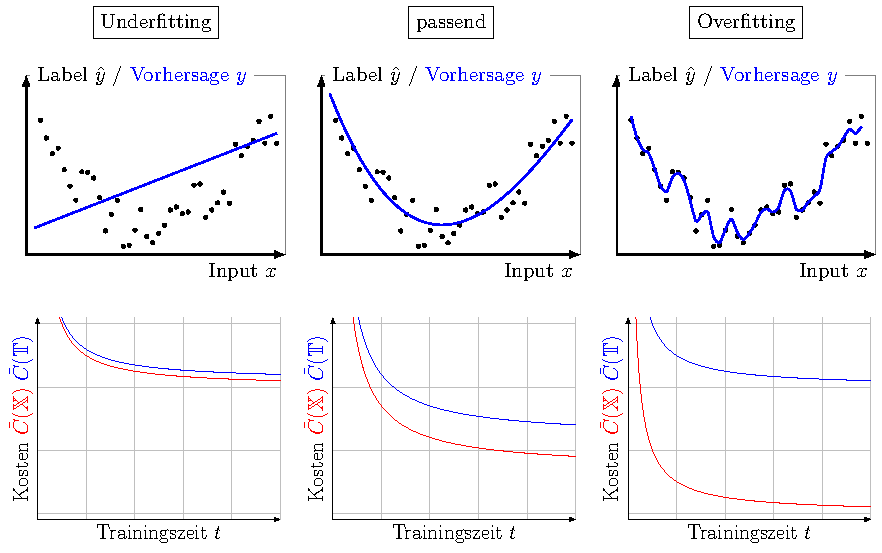
\includegraphics[width=0.9\textwidth]{fitting.pdf}
  \caption{Visualisierung von Under- und Overfitting}
\end{figure}
\para{}
Quellen: \cite{wiki:overfitting} \cite{Goodfellow-et-al-2016} \cite{book:hands-on}

% ------------------------------------------------------------

\chapter{Deep Learning und Künstliche Neuronale Netze}
Nach dem im ersten Kapitel die Basis für ein fundiertes Verständnis von
Maschinellem Lernen gelegt worden ist, soll es nun im zweiten Kapitel darum
gehen, ein spezifisches Modell, namentlich Künstliche Neuronale Netze, zu
erläutern. Darauf aufbauend wird in Kapitel drei die spezifische Architektur
eines Künstlichen Neuronalen Netzes, namentlich das Convolutional Neural Network,
dargelegt.
\para{}
\bigskip
Die wohl besten Resultate für die meisten Problemstellungen des Maschinellen Lernens (Bilderkennung,
Spracherkennung, etc.) werden durch \keyword{Künstliche Neuronale Netze} (engl.:
neural networks, kurz: KNN) geliefert.
Man bezeichnet diesen Bereich des Maschinellen Lernens auch als \keyword{Deep Learning}.
\para{}
Künstliche Neuronale Netze sind vor allem biologisch durch Nervensysteme von
Lebewesen inspiriert.
Sie sind aber lediglich eine Abstraktion dieser Informationsverarbeitung und
versuchen nicht eine möglichst genaue biologische Abbildung darzustellen.
Es gibt nicht nur eine Art von Neuronalem Netz, sondern es existieren die
verschiedensten Architekturen, welche je nach Problemstellung ausgewählt werden
müssen. Diese Arbeit wird vor allem von zwei solcher Architekturen Gebrauch machen:
Convolutional Neural Networks und sogenannte Autoencodern.

\para{}
Quellen: \cite{book:hands-on}

\section{Perzeptron}
Um den Aufbau und die Funktion eines Künstlichen Neuronalen Netzes besser zu
verstehen, wird im folgenden ein Vorgänger des KNN erklärt: das \keyword{Perzeptron}.
\para{}
Das einlagige Perzeptron wurde erstmals 1958 von Frank Rosenblatt vorgestellt. Dieses
besteht aus einem einzigen Künstlichen Neuron. Dieses künstliche Neuron
hat mehrere binäre Inputs und einen einzigen binären Output. Binär
bedeutet, dass der Wert nur entweder 0 (\textit{aus}) oder 1 (\textit{ein}) sein
kann. Des Weiteren besitzt es mehrere sogenannte \keyword{Gewichte} $w_1, \ldots,
w_m \in \set{R}$, für jeden Input $x_i$ ein Gewicht $w_i$.
Diese sind reelle Zahlen, welche das Verhalten des Perzeptron bestimmen.
Die \keyword{gewichtete Summe}, also die Summe aller Produkte der Inputs mit
ihrem Gewicht, wird mit $\tilde{z}$ bezeichnet.
Sie ist das gleiche wie das Skalarprodukt des Gewichtevektors
$\vec{w} = \trans{\begin{pmatrix} w_1 & \cdots & w_m \end{pmatrix}}$ mit dem
Inputvektor $\vec{x}$. \\
\begin{equation*}
  \tilde{z} = \sum_{i=1}^{m} w_i x_i = \vec{w} \cdot \vec{x}
\end{equation*} \\
Zusätzlich besitzt das Perzeptron einen \keyword{Schwellenwert} $\tilde{b}$.
Zusammen mit den Gewichten bilden sie die Modellparameter.
Das Perzeptron verhält sich so, dass falls die gewichtete Summe $\tilde{z}$ grösser als der
Schwellenwert $\tilde{b}$ ist, das Neuron feuert. Das bedeutet der Output beträgt 1;
andernfalls ist er 0 (siehe erster Teil der Hypothesenfunktion $h$ in Gleichung \refbox{eq:perzeptron_1}).
Es ist gängig, die Ungleichung der Bedingung in die Nullstellenform zu bringen
und $\tilde{b}$ durch die \keyword{Neigung} (engl.:\ bias)
$b = -\tilde{b}$ zu ersetzten. Somit lautet die Ungleichung: $\tilde{z} + b
> 0$. Der neue Term $\tilde{z} + b$ wird mit $z$ bezeichnet (siehe Rest der Gl. \refbox{eq:perzeptron_1}).
Die Neigung gibt an, wie stark das Neuron dazu neigt, zu feuern.\\

\begin{equation}\label{eq:perzeptron_1}
  h(\vec{x}) =
  \begin{cases}
    1 & \quad \text{falls } \tilde{z} > \tilde{b}\\
    0 & \quad \text{ansonsten}
  \end{cases}
  \quad =
  \begin{cases}
    1 & \quad \text{falls } z > 0\\
    0 & \quad \text{ansonsten}
  \end{cases}
  \quad =
  \begin{cases}
    1 & \quad\text{falls } \vec{w} \cdot \vec{x} + b > 0\\
    0 & \quad\text{ansonsten}
  \end{cases}
\end{equation}
\para{}
\begin{figure}[h!]
  \centering
  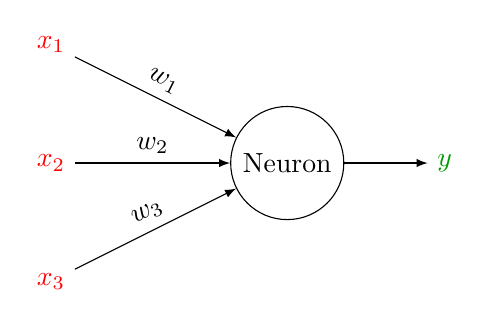
\begin{tikzpicture}[>=latex]
    \path (3,0) node [circle,draw](neuron){Neuron};
    \path[red] (0,1.5) node(x1){$x_1$} (0,0) node(x2){$x_2$} (0,-1.5) node(x3){$x_3$};
    \path[black!40!green] (5,0) node(y1){$y$};
    \draw[->] (x1) -- node[above,sloped]{$w_1$} (neuron);
    \draw[->] (x2) -- node[above,sloped]{$w_2$} (neuron);
    \draw[->] (x3) -- node[above,sloped]{$w_3$} (neuron);
    \draw[->] (neuron) -- (y1);
  \end{tikzpicture}
  \caption{Perzeptron mit drei Inputs}
  \label{fi:perzeptron}
\end{figure}
\para{}
Für das Trainieren des Perzeptrons existieren spezielle Verfahren, welche hier
aber nicht weiter beleuchtet werden sollen. Dies aus dem Grund, weil das
Gradientenverfahren hier nicht verwendet werden kann.
Der Grund dafür soll wird in Sektion \refbox{sec:heaviside} erläutert.
\para{}
Quellen: \cite{wiki:perzeptron} \cite{Nielsen} \cite{book:hands-on}

\subsection{Lernpotenzial eines Perzeptrons}
Nun stellt sich die Frage, was ein Perzeptron eigentlich erlernen kann und wofür
es nutzbar ist.
Das Perzeptron ist lediglich ein \keyword{linearer Klassifikator} der Form
$y = w_1x_1 + \cdots + w_m x_m$. Es ist also ein Klassifizierungsmodell und kein Regressionsmodell.
Es kann die Features in zwei Klassen 0 oder 1 einordnen, wobei der Output der
Hypothesenfunktion diese Klassifizierung angibt.
Überschreitet $y$ den Schwellenwert $\tilde{b}$, werden die Features der Klasse 1 zugeordnet, sonst
der Klasse 0.
Jedoch müssen diese Klassen linear separierbar sein.
\para{}
Lineare Separierbarkeit bedeutet, dass alle Featurevektoren $\vec{x}_1,\ldots,\vec{x}_p \in \set{R}^m$
innerhalb ihres Vektorraums $\set{R}^m$ durch eine Hyperebene in ihre Klassen aufteilbar sein müssen.
Falls das Perzeptron zwei Inputs besitzt, bedeutet dies, dass die Ortsvektoren
durch eine Gerade voneinander trennbar sein müssen (siehe Abb.
\refbox{fig:linearer_Klassifikator}). \\
Falls die Features nicht linear separierbar sind,
kann das Perzeptron die Klassifizierung nicht erlernen. Somit ist diese Modell
ziemlich primitiv und kann nicht auf komplizierte nicht-lineare Problemstellung
angewandt werden.
\\
\begin{figure}[h!]
  \centering
  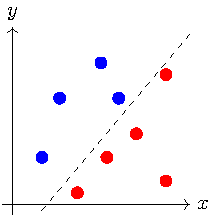
\includegraphics[width=0.3\textwidth]{sep.pdf}
  \caption{zwei-dimensionale lineare Separierung}
  \label{fig:linearer_Klassifikator}
\end{figure}
\para{}
Quellen: \cite{wiki:perzeptron} \cite{wiki:linear_separability}

\section{Erweiterung der künstlichen Neuronen}\label{sec:künstlicheNeuronen}
Ein Perzeptron ist, wie vorhin erklärt, nur in der Lage lineare Klassifikationen
durchzuführen. Um nun auch Regressionsprobleme zu lösen, muss das Konzept des
künstlichen Neurons ausgebaut werden. Wir benötigen ein Neuron, welches sich
besonders gut als Baustein für KNNs eignet.


\subsection{Künstliche Neuronen im Allgemeinen}
Künstliche Neuronen sind immer so aufgebaut, dass sie einen oder mehrere Inputs
und nur einen einzigen Output besitzen. Zu jedem Input $x_i$ ist ein Gewicht
$w_{i}$ assoziiert. Zuerst wird die gewichtete Summe der Inputs $\tilde{z}$ gebildet.
Die Neigung $b$ wird ebenfalls dazu addiert, um $z$ zu erhalten. Nun muss
die sogenannte \keyword{Aktivierung} $a$ gebildet werden. Sie ist der Output des Neurons.
Die Aktivierung $a = \varphi(z)$ ist das Resultat der
\keyword{Aktivierungsfunktion} $\varphi: \set{R} \to \set{R}$ angewendet
auf $z$. Die verschiedenen künstlichen Neuronen unterscheiden
sich fast nur in ihrer Aktivierungsfunktion.
\\
\begin{figure}[h!]
  \centering
  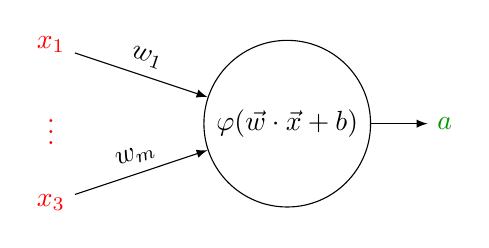
\begin{tikzpicture}[>=latex]
    \path (3,0) node [circle,draw](neuron){$\varphi(\vec{w} \cdot \vec{x} + b)$};
    \path[red] (0,1) node(x1){$x_1$} (0,0) node(x2){$\vdots$} (0,-1) node(x3){$x_3$};
    \path[black!40!green] (5,0) node(y1){$a$};
    \draw[->] (x1) -- node[above,sloped]{$w_1$} (neuron);
    \draw[->] (x3) -- node[above,sloped]{$w_m$} (neuron);
    \draw[->] (neuron) -- (y1);
  \end{tikzpicture}
  \caption{ein künstliches Neuron}
\end{figure}
\\

\para{}
Quellen: \cite{Nielsen} \cite{wiki:kuenstliches_neuron} \cite{book:hands-on}

\subsection{Perzeptronen als künstliche Neuronen}\label{sec:heaviside}
Nun nochmal ein Blick auf das Perzeptron im Angesicht der Aktivierungsfunktion.
Ein wesentlicher Unterschied des Perzeptrons gegenüber sonstigen künstlichen
Neuronen besteht darin, dass seine Inputs und Outputs nur binäre Werte
annehmen können. Um dieses Verhalten des Perzeptrons zu erhalten,
muss eine Stufenfunktion als Aktivierungfunktion verwendet werden: die Heaviside-Funktion $\Theta$.
Sie hat einen einzigen Stufensprung bei $x=0$ vom Wert 0 auf 1 (siehe Abb.
\refbox{fig:heaviside}). Eine Konsequenz dieser Stufenfunktion ist, dass das
Gradientenverfahren hier nicht angewendet werden kann, da die Ableitung der
Heaviside-Funktion entweder nicht definiert ist ($x=0$) oder überall 0 beträgt.
\\
\begin{figure}[h!]
  \begin{minipage}[h!]{0.5\textwidth}
    \begin{equation*}
      \varphi^{\text{hlim}}(z) = \Theta(z) =
      \begin{cases}
        1 & \quad \text{falls } z \geq 0\\
        0 & \quad \text{falls } z < 0
      \end{cases}
    \end{equation*}
  \end{minipage}
  \begin{minipage}[h!]{0.5\textwidth}
    \centering
    \begin{tikzpicture}[scale=2.5]
      \draw[->] (-1.5,0) -- (1.5,0) node[right] {$x$}; % x-axes
      \draw[->] (0,-0.2) -- (0,1.2) node [above] {$y$}; % y-axes
      \draw[style=help lines,step=0.5] (-1.4,0) grid (1.4, 1.1);

      \foreach \x in {-1,-0.5,0.5,1}
      \draw[shift={(\x,0)}] (0pt,2pt) -- (0pt,-2pt) node[below,fill=pagecolor] {$\x$};

      \foreach \y in {0.5,1}
      \draw[shift={(0,\y)}] (2pt,0pt) -- (-2pt,0pt) node[left,fill=pagecolor] {$\y$};

      \draw[shift={(0,0)}] (0pt,0pt) node[below left,fill=pagecolor] {$O$};

      \draw[red,ultra thick] (-1.5,0) -- (0,0); % 0-red
      \draw[red,ultra thick] (0,1) -- (1.5,1); % 1-red
      \draw[red,ultra thick,dashed] (0,0) -- (0,1); % y-red
      \draw[draw=red,fill=white] (0,0) circle (0.05);
      \draw[draw=red,fill=red] (0,1) circle (0.05);
    \end{tikzpicture}
  \end{minipage}
  \caption{Definition und Graph der Heaviside-Funktion $\Theta$}
  \label{fig:heaviside}
\end{figure}

\para{}
Quellen: \cite{wiki:kuenstliches_neuron} \cite{wiki:perzeptron} \cite{book:hands-on}

\subsection{ReLU-Neuronen}\label{sec:ReLU}
Der nächste Schritt nach einer Stufenfunktion als Aktivierungsfunktion, sind
lineare Aktivierungsfunktionen. Für diese können die Inputs nun beliebige reelle
Zahlen sein.
Jedoch sind solche lineare Neuronen in einem KNN von keinerlei Nutzen.
Dies ist dadurch begründet, dass eine Verkettung von linearen Neuronen
immer auf eine einzige lineare Funktion reduziert werden kann. Somit hat
die Verkettung keinen Mehrwert.
\para{}
Stattdessen verwendet man sogenannte ReLU-Neuronen. Sie benutzen die
\keyword{Rectified Linear Unit} (\keyword{ReLU}) als Aktivierungsfunktion.
Diese ist eine
nur teilweise lineare Aktivierungsfunktion. Die Werte grösser als 0 werden
auf sich selbst linear abgebildet und die Werte kleiner oder gleich 0 werden auf 0
abgebildet (siehe Abb. \refbox{fig:relu}).
Eine sehr wichtige Eigenschaft der ReLU-Funktion ist, dass sie - im Gegensatz zu der vorherigen
Heaviside-Funktion $\Theta$ - fast überall differenzierbar%
\footnote{%
  Eigentlich ist die ReLU-Funktion in $x=0$ wegen des Knicks nicht
  differenzierbar. Für die Gradientenberechnung definiert man jedoch einfach
  die Ableitung $\varphi'^{\text{ReLU}}(0) \coloneqq 0$. Dies ist mathematisch zwar nicht
  korrekt, löst aber das Problem.
}%
und monoton steigend ist. Erst für diese Aktivierungsfunktion kann das Gradientenverfahren
angewendet und somit das KNN trainiert werden.
\para{}
Da die ReLU-Funktion nur teilweise linear ist, gehört sie genau genommen den
nicht-linearen Aktivierungsfunktionen an. Diese Nicht-Linearität erlaubt es dem
Neuron, deutlich komplexere Systeme zu modellieren bzw. deutlich komplexere
Probleme zu lösen. In Sektion \refbox{sec:UAT} wird dargelegt, dass
eine Komposition von nicht-linearen Neuronen jede beliebige Funktion approximieren kann.
\para{}
Das ReLU-Neuron werden wir an dieser Stelle zur Seite legen und erst wieder in
Kapitel \refbox{sec:CNN} im Zusammenhang mit KNNs zur Bilderkennung betrachten.
\para{}
\begin{figure}[h!]
  \begin{minipage}[h!]{0.5\textwidth}
    \begin{equation}
      \varphi^{\text{ReLU}}(z) =
      \begin{cases}
        z & \quad \text{falls } z > 0\\
        0 & \quad \text{falls } z \leq 0
      \end{cases}
      = \max(z,0)
    \end{equation}
  \end{minipage}
  \begin{minipage}[h!]{0.5\textwidth}
    \centering
    \begin{tikzpicture}[scale=2.5]
      \draw[->] (-1.5,0) -- (1.5,0) node[right] {$x$}; % x-axes
      \draw[->] (0,-0.2) -- (0,1.2) node [above] {$y$}; % y-axes
      \draw[style=help lines,step=0.5] (-1.4,0) grid (1.4, 1.1);

      \foreach \x in {-1,-0.5,0.5,1}
      \draw[shift={(\x,0)}] (0pt,2pt) -- (0pt,-2pt) node[below,fill=pagecolor] {$\x$};

      \foreach \y in {0.5,1}
      \draw[shift={(0,\y)}] (2pt,0pt) -- (-2pt,0pt) node[left,fill=pagecolor] {$\y$};

      \draw[shift={(0,0)}] (0pt,0pt) node[below left,fill=pagecolor] {$O$};

      \draw[red,ultra thick] (-1.5,0) -- (0,0);
      \draw[red,ultra thick] (0,0) -- (1,1);
      \draw[red,ultra thick,dashed] (1,1) -- (1.2,1.2);

      \draw[draw=red,fill=red] (0,0) circle (0.03);
    \end{tikzpicture}
  \end{minipage}
  \caption{Formel und Graph der ReLU-Funktion}
  \label{fig:relu}
\end{figure}
\para{}
Quellen: \cite{wiki:kuenstliches_neuron} \cite{Nielsen} \cite{book:hands-on}

\subsection{Sigmoid-Neuronen}
Ein weiteres nicht-lineares Neuron sind sogenannte Sigmoid-Neuronen.
Die Bezeichnung stammt von ihrer Aktivierungsfunktion: der Sigmoidfunktion $\sigma$.
Sie sind die meist verwendeten Neuronen in klassischen KNNs.
Auch sie können aufgrund ihrer Nicht-Linearität zur Approximation jeder Funktion
verwendet werden. Sie weichst stark von der Linearität ab und ist
somit auch in der Lage komplexe Sachverhalte zu modellieren.
\para{}
Die Sigmoid-Funktion besitzt eine einzige Wendestelle $\sigma''(x=0)=0$ und hat
zwei Asymptoten, eine $\ds\lim_{x \to -\infty} \sigma(x)=0$
und eine zweite $\ds\lim_{x \to \infty} \sigma(x)=1$ (siehe Abb.
\refbox{fig:sigmoid}). Des Weiteren zeichnet sie sich durch eine vergleichsweise
einfache Ableitung aus.
\\
\begin{figure}[h!]
  \begin{minipage}[h!]{0.5\textwidth}
    \begin{align*}
      \varphi^{\text{sig}}(z) &= \sigma(z) = \frac{1}{1 + e^{-z}}\\
      \sigma'(z)&=\sigma(z)(1-\sigma(z))
    \end{align*}
  \end{minipage}
  \begin{minipage}[h!]{0.5\textwidth}
    \centering
    \begin{tikzpicture}[scale=2.5]
      \draw[->] (-1.5,0) -- (1.5,0) node[right] {$x$}; % x-axes
      \draw[->] (0,-0.2) -- (0,1.2) node [above] {$y$}; % y-axes
      \draw[style=help lines,ystep=0.5,xstep=0.25] (-1.4,0) grid (1.4, 1.1);

      \foreach \x/\xtext in {-1/-4,-0.5/-2,0.5/2,1/4}
      \draw[shift={(\x,0)}] (0pt,2pt) -- (0pt,-2pt) node[below,fill=pagecolor] {$\xtext$};

      \foreach \y in {0.5,1}
      \draw[shift={(0,\y)}] (2pt,0pt) -- (-2pt,0pt) node[left,fill=pagecolor] {$\y$};

      \draw[shift={(0,0)}] (0pt,0pt) node[below left,fill=pagecolor] {$O$};

      \draw[red,ultra thick,x=0.25cm] plot[domain=-6.0:6.0] (\x,{1/(1+exp(-\x)) });
    \end{tikzpicture}
  \end{minipage}
  \caption{Definition, Ableitung und Graph der Sigmoid-Funktion $\sigma$}
  \label{fig:sigmoid}
\end{figure}

\para{}
Quellen: \cite{wiki:kuenstliches_neuron} \cite{wiki:sigmoidfunktion} \cite{book:hands-on}


\section{Topologie der Künstlichen Neuronalen Netze}
Nun sollen die Sigmoid-Neuronen als Bausteine für Künstliche
Neuronale Netze Verwendung finden. Dazu werden sie miteinander verbunden und bilden so ein Netz,
ähnlich wie ein Nervensystem.
\para{}
Diese Neuronen sind in verschiedenen Schichten (engl.: layers)
arrangiert. Die erste bildet die \keyword{Inputschicht}. Sie beinhaltet die
Inputneuronen. Diese sind eigentlich keine richtigen
Neuronen, sondern eher Platzhalter für ihr jeweiliges Feature $x_i$. Als Letztes kommt die
\keyword{Outputschicht} mit den Outputneuronen, welche jeweils einen Outputwert $y_i$
besitzen. Dazwischen liegen die \keyword{Zwischenschichten} (engl.: hidden layers). Von ihnen kann es
beliebig viele geben, und in ihnen können beliebig viele Neuronen liegen.
Falls viele Zwischenschichten verwendet werden, bezeichnet man das Netzwerk als
``deep''. Daher rührt auch der Begriff des Deep Learning.
Den Aufbau eines KNN bezeichnet man als \keyword{Topologie} des Netzes. Die
Topologie umfasst viele Hyperparameter. Darunter sind zum Beispiel die Anzahl
der Zwischenschichten, wie auch
die Anzahl der Neuronen pro Schicht.
\para{}
Jedes Neuron aus einer Schicht ist mit jedem Neuron aus der nächsten Schicht über
Verbindungen gekoppelt. Alle Verbindungen besitzen ein Gewicht analog zu den Inputs des
Perzeptrons. Die Aktivierung, also der Output, eines Neurons wandert entlang den jeweiligen
Verbindungen zu allen Neuronen der nächsten Schicht und dienen als deren Input.
\para{}
In Abbildung \refbox{fig:nn_layers} ist ein Beispiel eines Neuronalen Netzes
abgebildet. In diesem Fall besitzt es sowohl 4 Inputs, als auch 4 Outputs. Es hat
ausserdem 3 Zwischenschichten. Die Erste und die Dritte haben jeweils 3 Neuronen
und die Zweite besitzt 4 Neuronen. \\

\begin{figure}[h!]
  \centering
  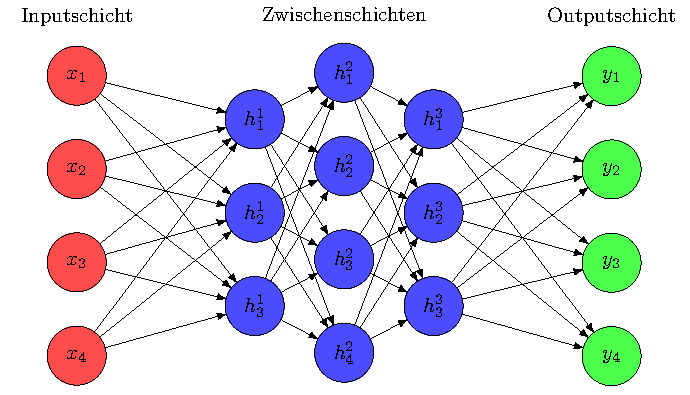
\includegraphics[width=0.8\textwidth]{knn1.pdf}
  \caption{Schichten eines KNNs}
  \label{fig:nn_layers}
\end{figure}

\para{}
Quellen: \cite{wiki:kuenstliches_neuronales_netz} \cite{Nielsen} \cite{book:hands-on}

\section{Lernverhalten}
Die Hoffnung beim Trainieren von KNNs besteht darin, dass das Modell für jede
weitere Schicht ein höheres Abstraktionsniveau erreicht. Würde man zum
Beispiel ein Netzwerk zur Gesichtserkennung trainieren, könnte man sich den
Erkennungsprozess folgendermassen vorstellen: Die erste Zwischenschicht erkennt
Kanten und Konturen. Die zweite vereint diese Merkmale zu Ecken und primitiven
geometrischen Formen. Die dritte Schichte sollte dann schon komplexere
geometrische Formen erkennen, welche gewissen Gesichtsmerkmalen, wie der Nase,
ähneln.
Die letzte Schichte soll dann alle diese
Merkmale zusammensetzen und so ein Gesicht als Ganzes erkennen.

\section{Vorwärtspropagierung}\label{sec:forward}
Jetzt, da der Aufbau eines KNNs erläutert wurde, soll die mathematische Funktionsweise
des Modells erklärt werden. Der Prozess der Berechnung der Outputwerte wird
\keyword{Vorwärtspropagierung} genannt. Dieses Verfahren gibt dieser Art von KNN auch den
Namen: \keyword{feedforward neural network}. Für das Verständnis müssen einige Konventionen zur
Bezeichnung der Teile eines KNNs getroffen werden. Es sollten zusätzlich noch
Abbildungen \refbox{fig:nomenklatur1} und \refbox{fig:nomenklatur2} zum besseren
Verständnis der Nomenklatur studiert werden.
\begin{itemize}
\item{$l$ ist der Index einer Schicht. Die Indexierung beginnt bei der
    Inputschicht mit 0.}
\item{$L$ ist der letzte Schichtindex und somit auch die gesamte Anzahl an
    Schichten (ohne die Inputschicht).}
\item{$|l|$ ist die Anzahl Neuronen in der $l$-ten Schicht%
    \footnote{
      Diese Schreibweise hat nichts mit dem Betrag zu tun, sondern wird
      gewählt, da sie sehr platzsparend ist.
    }.
  }
\item{$n_j^l$ bezeichnet das $j$-te Neuron in der $l$-ten Schicht.}
\item{$z_j^l$ ist die gewichtete Summe der Inputs des $j$-ten Neuron in der $l$-ten Schicht.}
\item{$a_j^l$ ist die Aktivierung (bzw. der Output) des $j$-ten Neurons in der $l$-ten Schicht.}
\item{$b_j^l$ ist die Neigung für das $j$-te Neuron in der ($l+1$)-ten Schicht%
    \footnote{
      Diese Konvention wurde gewählt, damit die folgenden Gleichungen simpler sind.
    }.
  }
\item{$w_{j,k}^l$ ist das Gewicht der Verbindung vom $k$-ten Neuron
    in der $l$-ten Schicht zum $j$-ten Neuron in der ($l+1$)-ten Schicht%
    \footnote{
      Man beachte die Reihenfolge der Indizes!\\
      Diese Konvention scheint zwar auf den ersten Blick unintuitiv, macht jedoch
      Sinn für die Matrixindexierung.
      \refbox{sec:backpropagation}.
    }.
  }
\item{$\varphi$ ist die gewählte Aktivierungsfunktion. Diese ist immer eine
    nicht-lineare Aktivierungsfunktion.}
\end{itemize}

\begin{figure}[h!]
  \centering
  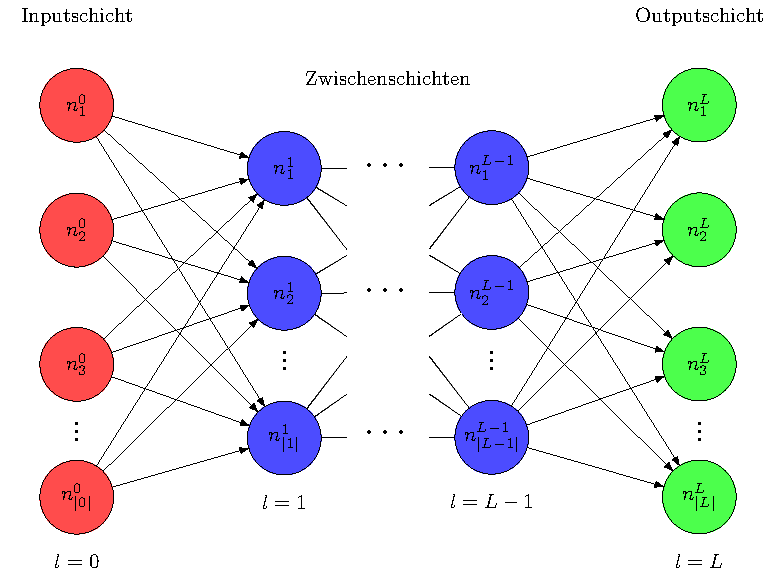
\includegraphics[width=0.8\textwidth]{knn2.pdf}
  \caption{zum Verständnis der Nomenklatur der Neuronen}
  \label{fig:nomenklatur1}
\end{figure}
\para{}
\begin{figure}[h!]
  \centering
  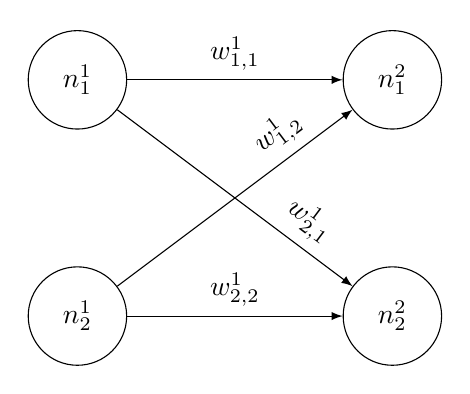
\begin{tikzpicture}[>=latex]
    \path (-2,1.5) node [draw,circle,inner sep=0,minimum size=1.25cm](n11){$n^1_1$};
    \path (-2,-1.5) node [draw,circle,inner sep=0,minimum size=1.25cm](n12){$n^1_2$};
    \path (2,1.5) node [draw,circle,inner sep=0,minimum size=1.25cm](n21){$n^2_1$};
    \path (2,-1.5) node [draw,circle,inner sep=0,minimum size=1.25cm](n22){$n^2_2$};
    \draw[->] (n11) -- node[above,sloped]{$w^1_{1,1}$} (n21);
    \draw[->] (n11) -- node[above,pos=0.75,sloped]{$w^1_{2,1}$} (n22);
    \draw[->] (n12) -- node[above,pos=0.75,sloped]{$w^1_{1,2}$} (n21);
    \draw[->] (n12) -- node[above,sloped]{$w^1_{2,2}$} (n22);
  \end{tikzpicture}
  \caption{zum Verständnis der Gewichtebeschriftungen}
  \label{fig:nomenklatur2}
\end{figure}
\para{}
Die Vorwärtspropagierung beginnt bei den Inputneuronen, welche jeweils
einen Inputwert in sich tragen. Diese Werte werden, um für eine kohärente Nomenklatur zu sorgen,
analog zu den Aktivierungen der anderen Neuronen mit $a_j^0$ bezeichnet, wobei
$j$ der Index des Neurons ist.
\para{}
Nun müssen die restlichen Aktivierungen der Neuronen bis und mit den
Ouputneuronen berechnet werden. Dies geschieht rekursiv, anhand der
Aktivierungen der vorherigen Schicht, und zwar folgendermassen (ersichtlich in
Gleichung \refbox{eq:gewichtete_summe_normal}):\\
Zuerst läuft eine Summe über alle Neuronen $n_k^{l}$ der jetzigen Schicht
$l$. Dabei wird die gewichtete Summe der Aktivierungen $a_k^{l}$ mit den
assoziierten Gewichten $w_{j,k}^l$ gebildet. Hierbei ist das Gewicht jenes, welches das
$k$-te Neuron der $l$-ten Schicht mit dem $j$-ten Neuron der ($l+1$)-ten Schicht
verbindet (siehe Abb. \refbox{fig:nomenklatur2}).
Zusätzlich gehört zu der gewichteten Summe auch die jeweilige Neigung $b_j^l$, welche
dazu addiert wird. Diese gewichtete Summe wird mit $z_j^{l+1}$ bezeichnet.
\\
\begin{equation}\tag{FP1}\label{eq:gewichtete_summe_normal}
  z_j^{l+1} = \sum_{k=1}^{|l|} w_{j,k}^l a_k^l + b_j^l
\end{equation}
\\
Auf diese Summe wird dann die Aktivierungsfunktion $\varphi$ angewandt.
Das ist dann die Aktivierung $a_j^{l+1}$ des $j$-ten Neurons in der ($l+1$)-ten Schicht.
\\
\begin{equation}\tag{FP2}\label{eq:aktivierung_normal}
  a_j^{l+1} = \varphi\left(\sum_{k=1}^{|l|} w_{j,k}^l a_k^{l} + b_j^l \right) = \varphi \left( z_j^{l+1} \right)
\end{equation}
\par\bigskip
Für Deep Learning braucht man vor allem sogenannte Deep Neural Networks. Diese
zeichnen sich dadurch aus, dass sie sehr viele Zwischenschichten besitzen.
Deshalb bezeichnet man sie als ``deep''.
Bei solchen Netzwerken ist es nicht unüblich,
dass sie sehr viele Neuronen und Verbindungen (über 100'000) besitzen.
Um hier nicht den Überblick zu verlieren bzw. damit nicht zu viele Indizes notwendig
sind, macht man Gebrauch von \keyword{Linearer Algebra}. Man verwendet
Matrizen und Vektoren, um die vielen Variablen zusammenzufassen.
Ausserdem besteht ein weiterer Vorteil darin, dass Computer mithilfe von Vektor-
und Matrixoperationen die Berechnungen parallelisieren können und in kürzerer
Zeit und mit weniger Ressourcen viele Berechnungen gleichzeitig ausführen können.
Dies beschleunigt das Training der Modelle um
ein Vielfaches. In Anhang \refbox{sec:anhang_tf} wird dies thematisiert.
\para{}
Die Inputs $\vec{x}$, Vorhersagen $\vec{y}$ und Labels $\vec{\hat{y}}$ wurden
bereits zu Beginn als Vektoren geschrieben.
Nun sollen noch die Modellparameter und die restlichen Komponenten eines KNNs als Vektoren und Matrizen zusammengefasst werden.
Sowohl alle gewichteten Summen $z_j^l$, wie auch alle Aktivierungen $a_j^l$
einer Schicht $l$, werden in Vektoren $\vec{z}^l \in \set{R}^{|l|}$ und
$\vec{a}^l \in \set{R}^{|l|}$ zusammengefasst.
Auch alle Neigungen $b_j^l$ für eine Schicht ($l+1$) bilden einen Vektor
$\vec{b}^l \in \set{R}^{|l+1|}$.
\para{}
Zu guter Letzt, wird noch eine \keyword{Gewichtsmatrix} $\mat{W}^l \in
\set{R}^{|l+1| \times |l|}$
definiert. Sie enthält alle Gewichte, welche die $l$-te
Schicht \textit{zu} der ($l+1$)-ten Schicht verbindet.
Das heisst, der Eintrag in der $j$-ten Zeile und in
der $k$-ten Spalte ist $w_{j,k}^l$ und verbindet so das Neuron $n_k^{l}$ zu
dem Neuron $n_j^{l+1}$.
\\
\begin{align*}
  \vec{z}^l &=  \trans{\begin{pmatrix} z_1^l & z_2^l & \cdots & z_{|l|}^l \end{pmatrix}} \\
  \vec{a}^l &=  \trans{\begin{pmatrix} a_1^l & a_2^l & \cdots & a_{|l|}^l \end{pmatrix}} \\
  \vec{b}^l &=  \trans{\begin{pmatrix} b_1^l & b_2^l & \cdots & b_{|l+1|}^l \end{pmatrix}} \\
\end{align*}
\begin{equation*}
  \mat{W}^l =
  \begin{pmatrix}
    w_{1,1}^l & w_{1,2}^l & \cdots & w_{1,|l|}^l \\[0.3em]
    w_{2,1}^l & w_{2,2}^l & \cdots & w_{2,|l|}^l \\[0.3em]
    \vdots & \vdots & \ddots & \vdots \\[0.3em]
    w_{|l+1|,1}^l & w_{|l+1|,2}^l & \cdots & w_{|l+1|,|l|}^l
  \end{pmatrix}
\end{equation*}
\\
Mit diesen Definitionen kann Gleichung \refbox{eq:gewichtete_summe_normal} in
Matrixform geschrieben werden. Dies, weil die Matrixmultiplikation von $\mat{W}^l$ mit
$\vec{a}^{l}$ einen Vektor $\vec{\tilde{z}}^{l+1}$ ergibt, welcher alle gewichteten
Summen $\tilde{z}_j^{l+1}$ ohne die jeweilige Neigung enthält.
\\
\begin{equation*}
  \mat{W}^l \vec{a}^{l} = \trans{\begin{pmatrix}\ds \sum_{j=1}^{|l|} w_{1,j}^l a_j^l &\ds \sum_{j=1}^{|l|} w_{2,j}^l a_j^l & \cdots &\ds \sum_{j=1}^{|l|} w_{|l+1|,j} a_j^l \end{pmatrix}} = \vec{\tilde{z}}^{l+1}
\end{equation*}
\\
Nun muss noch der Neigungsvektor $\vec{b}^l$ dazu addiert werden, damit die
Gleichung \refbox{eq:gewichtete_summe_matrix} entsteht, mit welcher der
Vektor der gewichteten Summen $\vec{z}^{l+1}$ gebildet werden kann.
\\
\begin{equation}\tag{FP1a}\label{eq:gewichtete_summe_matrix}
  \vec{z}^{l+1} = \mathbf{W}^{l} \vec{a}^{l} + \vec{b}^{l}
\end{equation}
\\
Im letzten Schritt wird die Aktivierungsfunktion auf $\vec{z}^{l+1}$
angewendet, um den Aktivierungsvektor $\vec{a}^{l+1}$ zu bilden.
Hierfür muss aber noch ein neues mathematisches
Konzept eingeführt werden: die Vektorisierung einer Funktion.
\para{}

\begin{defbox}{Vektorisierung einer Funktion}
  Die Vektorisierung einer skalaren Funktion $f$, geschrieben als
  $\vecf{f}[\vec{v}]$ hat als Argument einen Vektor $\vec{v}$, auf dessen
  Komponenten jeweils \textit{einzeln} die Funktion $f$ angewendet wird. Dieser neue
  Vektor ist der Rückgabewert der Funktion. Er besitzt die gleichen Dimensionen
  wie der Argumentvektor.
  \\
  \begin{equation*}
    \vecf{f}[\vec{v}]=
    \begin{pmatrix}
      f(v_1)\\
      \vdots \\
      f(v_n)\\
    \end{pmatrix}
  \end{equation*}
\end{defbox}
\para{}
Nun kann die vektorisierte Aktivierungsfunktion $\vecf{\varphi}$ auf
$\vec{z}^{l+1}$ angewendet werden.

\begin{equation}\tag{FP2a}\label{eq:aktivierung_matrix}
  \vec{a}^{l+1} = \vecf{\varphi} \left[\mat{W}^{l} \vec{a}^{l} + \vec{b}^{l} \right] = \vecf{\varphi} \left[ \vec{z}^{l+1} \right]
\end{equation}

\para{}
Quellen: \cite{Nielsen}

\subsection{Initialisierung der Modellparameter}\label{sec:parameter_initialisieren}
Ein weiterer Schritt, der vollzogen werden muss, bevor das Training beginnen kann, ist das
Initialisieren aller Modellparameter, in diesem Fall die Gewichte und Neigungen.
Dies ist ein sehr essenzieller Schritt, da diese Initialwerte die
Leistungsfähigkeit des Modells erheblich beeinflussen.
\para{}
Wie in Sektion \refbox{sec:gradientenverfahren} gezeigt, muss am Anfang des
Gradientenverfahrens ein Startpunkt $\vec{\param}_{t=0} = \trans{\begin{pmatrix}
    \param_1 & \cdots & \param_k \end{pmatrix}}$ innerhalb des Gradientenfeldes
$\vecf{\nabla}C$ gewählt werden, von welchem aus der Gradientenabstieg beginnt.
Dieser Startpunkt entscheidet darüber, in welches lokale Minimum konvergiert
wird und bestimmt somit auch die bestmögliche Exaktheit der Vorhersagen. Falls
schlechte Initialwerte gewählt wurden, konvergiert der Punkt in ein hohes lokales
Minimum, was grosse Kostenfunktionswerte und schlechte Vorhersagen verursacht.
\para{}
Es ist nicht möglich, im Vorhinein zu wissen, welche Initialwerte gute Resultate
liefern. Es müssen verschiedene Werte ausprobiert werden. Dafür initialisiert man gängigerweise die
Modellparameter mit Zufallswerten. Zu diesem Zweck werden nicht irgendwelche
Zufallsvariablen verwendet, sondern es gelangt die Gauss'sche Normalverteilung
$\mathcal{N}(\mu,\sigma^2)$ bzw. ihre Dichtefunktion (siehe Abb. \refbox{fig:normalverteilung}) zur Anwendung. Diese ist
folgendermassen definiert:
\[\ds \phi(x\ |\ \mu,\sigma^2) = \frac{1}{\sqrt{2\pi\sigma^2}} \text{exp} \left\{-\frac{{(x-\mu)}^2}{2\sigma^2}\right\} \]
\para{}
\begin{figure}[h!]
  \centering
  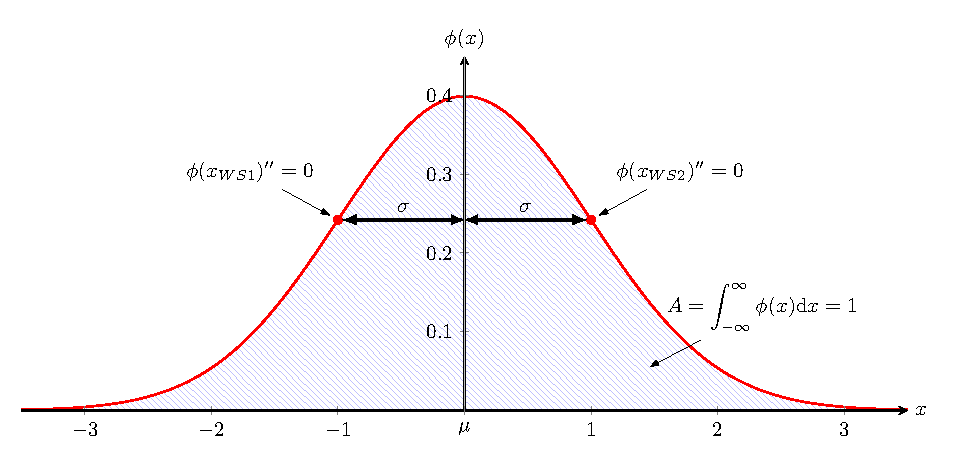
\includegraphics[width=0.8\textwidth]{gauss.pdf}
  \caption{Graph der Dichtefunktion $\phi(x\ |\ \mu=0,\sigma^2=1)$ mit ihren
    wichtigsten Eigenschaften}%
  \label{fig:normalverteilung}
\end{figure}
In den Anfängen des Maschinellen Lernens wurde häufig die normierte
Normalverteilung verwendet. Jedoch hatte dies zur Konsequenz, dass mit jeder Schicht die
Outputs eine stetig grösser werdende Standardabweichung $\sigma$ aufwiesen.
In Kombination mit Sigmoid-Neuronen, kommt es zu einer Verlangsamung des
Lernprozesses. Dieses Problem ist als das \keyword{Vanishing-Gradient-Problem} bekannt,
auf welches hier nicht weiter eingegangen wird.
\para{}
In der Konsequenz wurde eine neue Technik entwickelt: die \keyword{Glorot-Initialisierung}
(auch Xavier-Initialisierung genannt). Dabei gelangt erneut eine Normalverteilung
mit Erwartungswert $\mu = 0$ zur Anwendung. Die Standardabweichung $\sigma$ wird
anhand der Grösse einer Schicht skaliert.
Für eine Schicht $l$ wird der Durchschnitt zwischen der Anzahl Inputs
und der Anzahl Neuronen einer Schicht berechnet $r = \frac{|l-1| + |l|}{2}$. Der Kehrwert
davon ist die Varianz der Normalverteilung.
Die Gewichte werden folgendermassen initialisiert:
\begin{equation}
  w_{t=0}^l \sim \mathcal{N}\left(\mu = 0, \sigma^2 = \frac{2}{|l-1| + |l|}\right)
\end{equation}
Durch dieses Verfahren bleibt die Varianz innerhalb einer Schicht erhalten.
Teilweise wird dieses Verfahren auch für die Neigungen $b$ angewendet. Eine
andere Möglichkeit besteht in der Initialisierung der Neigungen mit 0, wie wir
das machen werden.
\begin{equation}
  b_{t=0}^l = 0
\end{equation}

\para{}
Quellen: \cite{wiki:normal_distribution} \cite{Nielsen} \cite{book:hands-on}

\section{Rückwärtspropagierung}\label{sec:backpropagation}
Ein KNN wird üblicherweise, wie die meisten Modelle, mithilfe des Stochastischen
Gradientenverfahrens trainiert.
Die wahre Herausforderung besteht darin, die partiellen Ableitungen der
Kostenfunktion bezüglich der Modellparameter zu berechnen.
Anders gesagt müssen alle Terme
$\ds\partderiv{C}{w_{j,k}^l}$, wie auch alle Terme $\ds\partderiv{C}{b_k^l}$,
bestimmt werden.
Das Verfahren zur Ermittlung dieser Ausdrücke in KNNs ist so spezifisch und aufwendig,
dass es einen eigenen Namen besitzt: die sogenannte \keyword{Rückwärtspropagierung} (engl.: backpropagation, auch
Fehlerrückführung).
\para{}
Für das Verständnis von ML ist es nicht essenziell, die Rückwärtspropagierung zu
verstehen. Jedoch kann so nachvollzogen werden, wie SGD in der Praxis funktioniert.
Grob umrissen besteht der Grundgedanke darin, die Werte der Kostenfunktion
rückwärts durch das Modell zu schicken und dabei die partiellen Ableitungen
mithilfe der Kettenregel zu bestimmen. Daher hat das Verfahren auch seinen Namen.
\para{}
Für eine ausführliche Herleitung ist auf Anhang
\refbox{sec:anhang_bp} zu verweisen, in welchem ebenfalls auf das Konzept eines
Computational Graphs eingegangen wird.

\section{Universal Approximation Theorem}\label{sec:UAT}
Es stellt sich nun die Frage, was ein Neuronales Netz alles erlernen kann.
Diese Frage kann mithilfe des \keyword{Universal Approximation Theorem} (UAT)
beantwortet werden. Es handelt sich um einen mathematischen Beweis dafür, dass ein KNN
grundsätzlich in der Lage ist, jede kontinuierliche Funktion beliebig exakt zu
approximieren.
\para{}
Etwas genauer ausgedrückt, besagt der UAT, dass ein KNN mit einer einzigen
Zwischenschicht, welche eine endliche Anzahl Neuronen besitzt, sich jeder kontinuierlichen
Funktion beliebig stark annähern kann. Voraussetzung dafür ist, dass es sich bei den
Neuronen um nicht-lineare Neuronen handelt.
Da sich die meisten Klassen von Problemen als eine Funktion formulieren
lassen, bedeutet dies, dass ein KNN theoretisch jedes Problem lösen kann!
Jedoch handelt es sich beim UAT nur um eine theoretische
Aussage über das Lernpotenzial eines KNNs. Somit trifft das Theorem keinerlei Aussage
darüber, ob ein KNN wirklich erfolgreich darin ist, die jeweilige Funktion zu erlernen.
Ein mögliches Hindernis könnte in Overfitting bestehen.
\para{}
Da der eigentliche Beweis mathematisch ziemlich anspruchsvoll ist, wird er im
Rahmen dieser Arbeit nicht weiter behandelt.
\para{}
Quellen: \cite{Nielsen} \cite{wiki:uat}


\pagebreak
\chapter{Convolutional Neural Networks}\label{sec:CNN}
Nachdem in Kapitel zwei das Wesen von Künstlichen Neuronalen Netzen
charakterisiert wurde, soll es nun in Kapitel drei darum gehen, eine spezifische
Architektur eines KNNs zu erklären, welche sich besonders gut für Bilderverarbeitung eignet.
Es handelt sich um das Convolutional Neural Network.
\para{}
\bigskip
Viele Anwendungen von Machine Learning sind mit einer Bild- oder
Audioverarbeitung verbunden, wie z. B.Bildklassifizierung, Gesichts- oder
Spracherkennung.
Vor allem für hochauflösende Bilder sind die KNNs, wie wir sie soeben
kennengelernt haben, jedoch nicht geeignet. Sie sind zum Teil gar nicht in der
Lage, eine Korrelation zwischen den Inputs und Outputs zu erlernen.
Um diesen Umstand zu erklären, wird ein kleines Beispielmodell erläutert:
\para{}
\label{sec:CNN_parameter_problem}
Es soll ein KNN entworfen werden, welches eine Photographie danach klassifizieren
soll, ob ein Hund darauf sichtbar ist oder nicht. Für dieses
Gedankenexperiment wird ein relativ niedrig aufgelöstes Bild mit $256 \times 256$
Pixel gewählt (dies entspricht weniger als $0.07$ Megapixel; im Vergleich dazu:
Ein iPhone XS hat eine Kamera mit 12 Megapixel). Um die verschiedenen Farben zu codieren, besitzt jeder Pixel drei
Farbkomponenten: R (rot), G (grün)
und B (blau). Somit hat dieses Bild insgesamt $256 \times 256 \times 3 = 196'608$
Komponenten. Jede Komponente ist ein Feature, welches das KNN zu verarbeiten hat. So bestünde
die erste Schicht des Netzwerkes aus fast $200'000$ Neuronen. Um diese Schicht
nun mit seiner Nachbarsschicht zu verbinden, welche die gleiche Grösse besitzt, werden
$196'608 \times 196'608 = 38'654'705'664$ Verbindungen und damit gleich
viele Gewichte benötigt! Für ein Netzwerk ohne eine einzige Zwischenschicht gäbe es
also über 38 Milliarden Modellparameter zu erlernen! Dass dies nicht realistisch ist,
liegt auf der Hand.
\para{}
Nicht nur die Anzahl der Modellparameter ist ein Problem für KNNs in der
Bildverarbeitung, sondern es existieren noch weiter Probleme.
Ohne auf diese einzugehen, sollte nun klar sein, dass eine andere Modellarchitektur notwendig ist, um Machine
Learning auf Bilder anwenden zu können. Für derartige Anwendungen wurde eine modifizierte
Version eines KNNs entwickelt: das \keyword{Convolutional Neural Network} (CNN).
Im Allgemeinen sind CNNs immer dann geeignet, wenn es Daten zu verarbeiten gilt, welche eine
rasterartige Form aufweisen, wie z. B.Bilder.
Diese Art von Netzwerk macht Gebrauch von Konzepten aus der klassischen
Bildverarbeitung, wie sie beispielsweise auch Photoshop ermöglicht.
Wie beim Perzeptron und bei den klassischen KNNs wurde auch hier die Architektur
von der Biologie inspiriert.
Der folgende Abschnitt wird die Funktionsweise eines solchen CNNs erklären.
\para{}
Quellen: \cite{Goodfellow-et-al-2016} \cite{deeplearning.ai:cnn} \cite{wiki:cnn}


\section{Bilder als Tensoren}\label{sec:tensor}
CNNs verarbeiten Bilder. Diese stellen den Input für die Modelle dar.
Um diese Bilder erfassen zu können, ist es sinnvoll, sie als sogenannte
\keyword{Tensoren} vom Rang 3 zu untersuchen, anstatt sie als Anordnungen von
Pixeln zu betrachten. Um zu verstehen, was ein Tensor dritten Ranges ist,
soll zunächst erläutert werden, was mit einem Tensor im Allgemeinen gemeint ist.

\begin{defbox}{Tensor}
  Ein Tensor $\ten{T}$ ist eine Verallgemeinerung von Skalaren, Vektoren und Matrizen auf
  $n$ Dimensionen. Es handelt sich wie bei Matrizen um
  eine Zahlenanordnung. Dabei wird die Anzahl Dimensionen, innerhalb welcher die
  Zahlen liegen, als Rang oder Stufe $n$ des Tensors bezeichnet. Vorstellen kann man sich einen Tensor
  als ein Hyperrechteck mit $n$ Dimensionen, innerhalb dessen die Zahlen in
  einem Raster angeordnet sind. Diese Zahlen sind die Elemente des Tensors.
  Ein Tensor nullten Ranges ist ein Skalar, ein Tensor ersten Stufe ist ein
  Vektor und ein Tensor mit Rang 2 ist eine normale 2D-Matrix.
  \begin{gather*}
    1 \in \set{R} \text{ (Skalar)} \quad \begin{pmatrix} 1 \\ 2 \\ 3 \end{pmatrix}
    \in \set{R}^3 \text{ (Vektor)} \quad
    \begin{pmatrix}
      1 & 2 & 3 \\
      4 & 5 & 6 \\
    \end{pmatrix} \in \set{R}^{2 \times 3} \text{ (Matrix)}
  \end{gather*}
\end{defbox}

\begin{defbox}{Tensor 3. Ranges}
  Ein Tensor $\ten{T} \in \set{R}^{h \times w \times d}$ mit Rang 3 ist eine 3-dimensionale Zahlenanordnung. Man kann sich
  diesen Tensor als eine 3D-Matrix vorstellen; ein Volumen, innerhalb
  dessen die Elemente in einem Raster angeordnet sind.
  Analog zum Volumen bezeichnet man die Form des Tensors mit Höhe, Breite und
  Tiefe.
  \para{}
  Die Schreibweisen-Konvention für Tensoren 3. Ordnung soll an folgendem
  Beispielstensor der Form $\set{R}^{3 \times 3 \times 3}$ illustriert werden. \\
  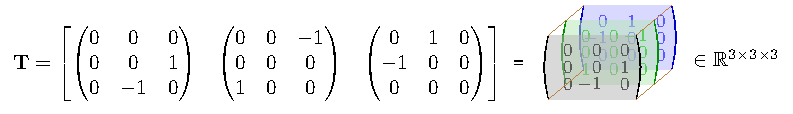
\includegraphics[width=0.8\textwidth]{tensor.pdf}

\end{defbox}
\para{}
Ein Bild kann somit als Tensor dritten Ranges $\ten{B} \in \set{R}^{h
  \times w \times c}$ betrachtet werden, in der Form $(\text{Bildhöhe} \times \text{Bildbreite}
\times \text{Anzahl Farbkomponenten})$.
Die Elemente der Matrix nehmen dann die Werte der Pixelkomponenten an.
Ein schwarz-weisses Bild hat nur eine Komponente, welche die Helligkeit angibt.
Somit wäre es eine normale 2D-Matrix $\mat{B} \in \set{R}^{h \times w}$.
\para{}
Quellen: \cite{deeplearning.ai:cnn} \cite{wiki:tensor}

\section{Topologie der Convolutional Neural Networks}
Ein CNN besteht, wie ein KNN auch, aus mehreren Schichten. Jede dieser Schichten erhält
als Input ein Bild und hat auch wieder eines als Output.
Ein wichtiger Unterschied des CNNs ist, dass es aus unterschiedlichen Typen von
Schichten besteht. Grundsätzlich lassen sich vier Arten von Schichten unterscheiden:
\begin{itemize}
\item{\keyword{Fully-connected-Schichten}}
\item{\keyword{Convolutional-Schichten}}
\item{\keyword{Pooling-Schichten}}
\item{\keyword{Upsampling-Schichten}}
\end{itemize}
Die Fully-Connected-Schicht ist bereits bekannt und verkörpert die klassische Schicht
eines KNNs, bestehend aus Neuronen. Auf diese werden wir daher nicht weiter eingehen,
da sie bereits im vorherigen Kapitel erläutert wurde.
\para{}
Die Convolutional-Schicht ist eine neuartige Schicht, welche es im KNN nicht
gibt. Sie ist die Schicht, welche für das Training relevant ist,
da sie die Modellparameter beinhaltet. Sie extrahiert die relevanten Features
aus den Inputbildern und lernt so die Bilder zu verstehen.
\para{}
Die Pooling-Schichten, wie auch die Upsampling-Schichten, beinhalten keine
Modellparameter und sind deshalb für das Training nicht direkt relevant.
Diese Schichten werden lediglich benötigt, um die verarbeiteten Bilder neu zu
skalieren. Dies ist sinnvoll, da durch die Extraktion gewisser Features die
restlichen Features wegfallen. Somit muss weniger Information pro Bild gespeichert
werden und die Bilder sollten schrumpfen, um Overfitting vorzubeugen. Die Pooling-
Schichten reduzieren die Bilder und die Upsampling-Schichten erweitern sie.
Dies wird in Sektion \refbox{sec:autoencoder} für die Entwicklung von Autoencoder
hilfreich werden. \\
Grundsätzlich folgt auf eine Convolutional-Schicht entweder eine Pooling-
oder eine Upsampling-Schicht. Somit bilden sie gewissermassen eine Einheit.
\para{}
Quellen: \cite{Goodfellow-et-al-2016} \cite{deeplearning.ai:cnn} \cite{wiki:cnn}


\section{Convolutional-Schichten und Filter}
Zuerst wird nun die Convolutional Schicht betrachtet. Diese Schicht macht ausgiebig
Gebrauch von sogenannten Filtern. Diese werden in diesem Abschnitt ausführlich behandelt.

\subsection{Filter in der Bildverarbeitung}
\keyword{Filter} (auch Kerne) sind in der Bildverarbeitung sehr verbreitet. Jeder kennt sie entweder
von Photoshop, von Instagram oder sonstigen Bildbearbeitungsprogrammen.
Auch CNNs machen Gebrauch von solchen Filtern. In diesem Fall, um die Features eines Bildes zu
erlernen.

\begin{figure}[h!]
  \centering
  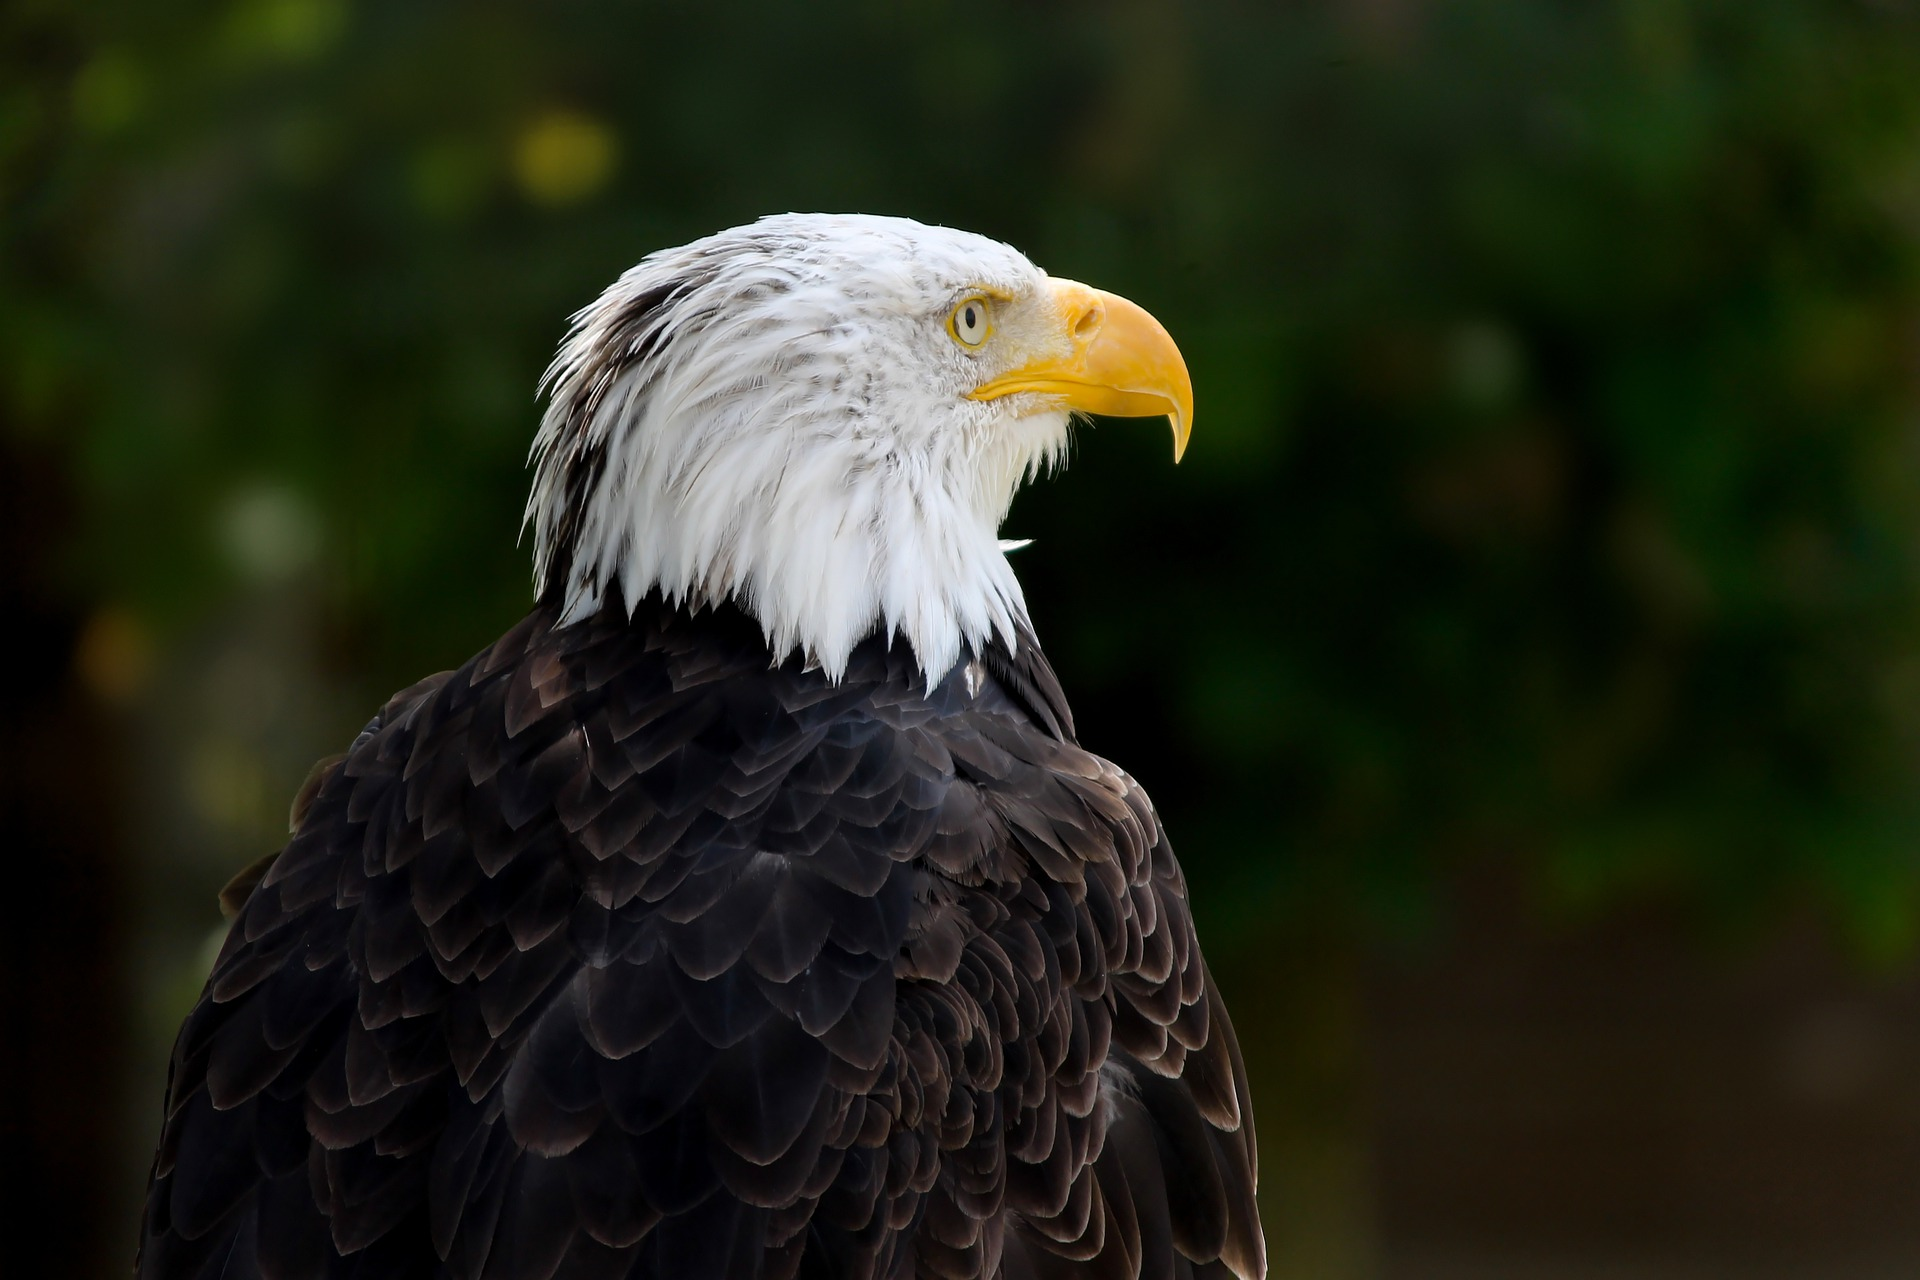
\includegraphics[width=0.4\textwidth]{eagle-color.jpg}
  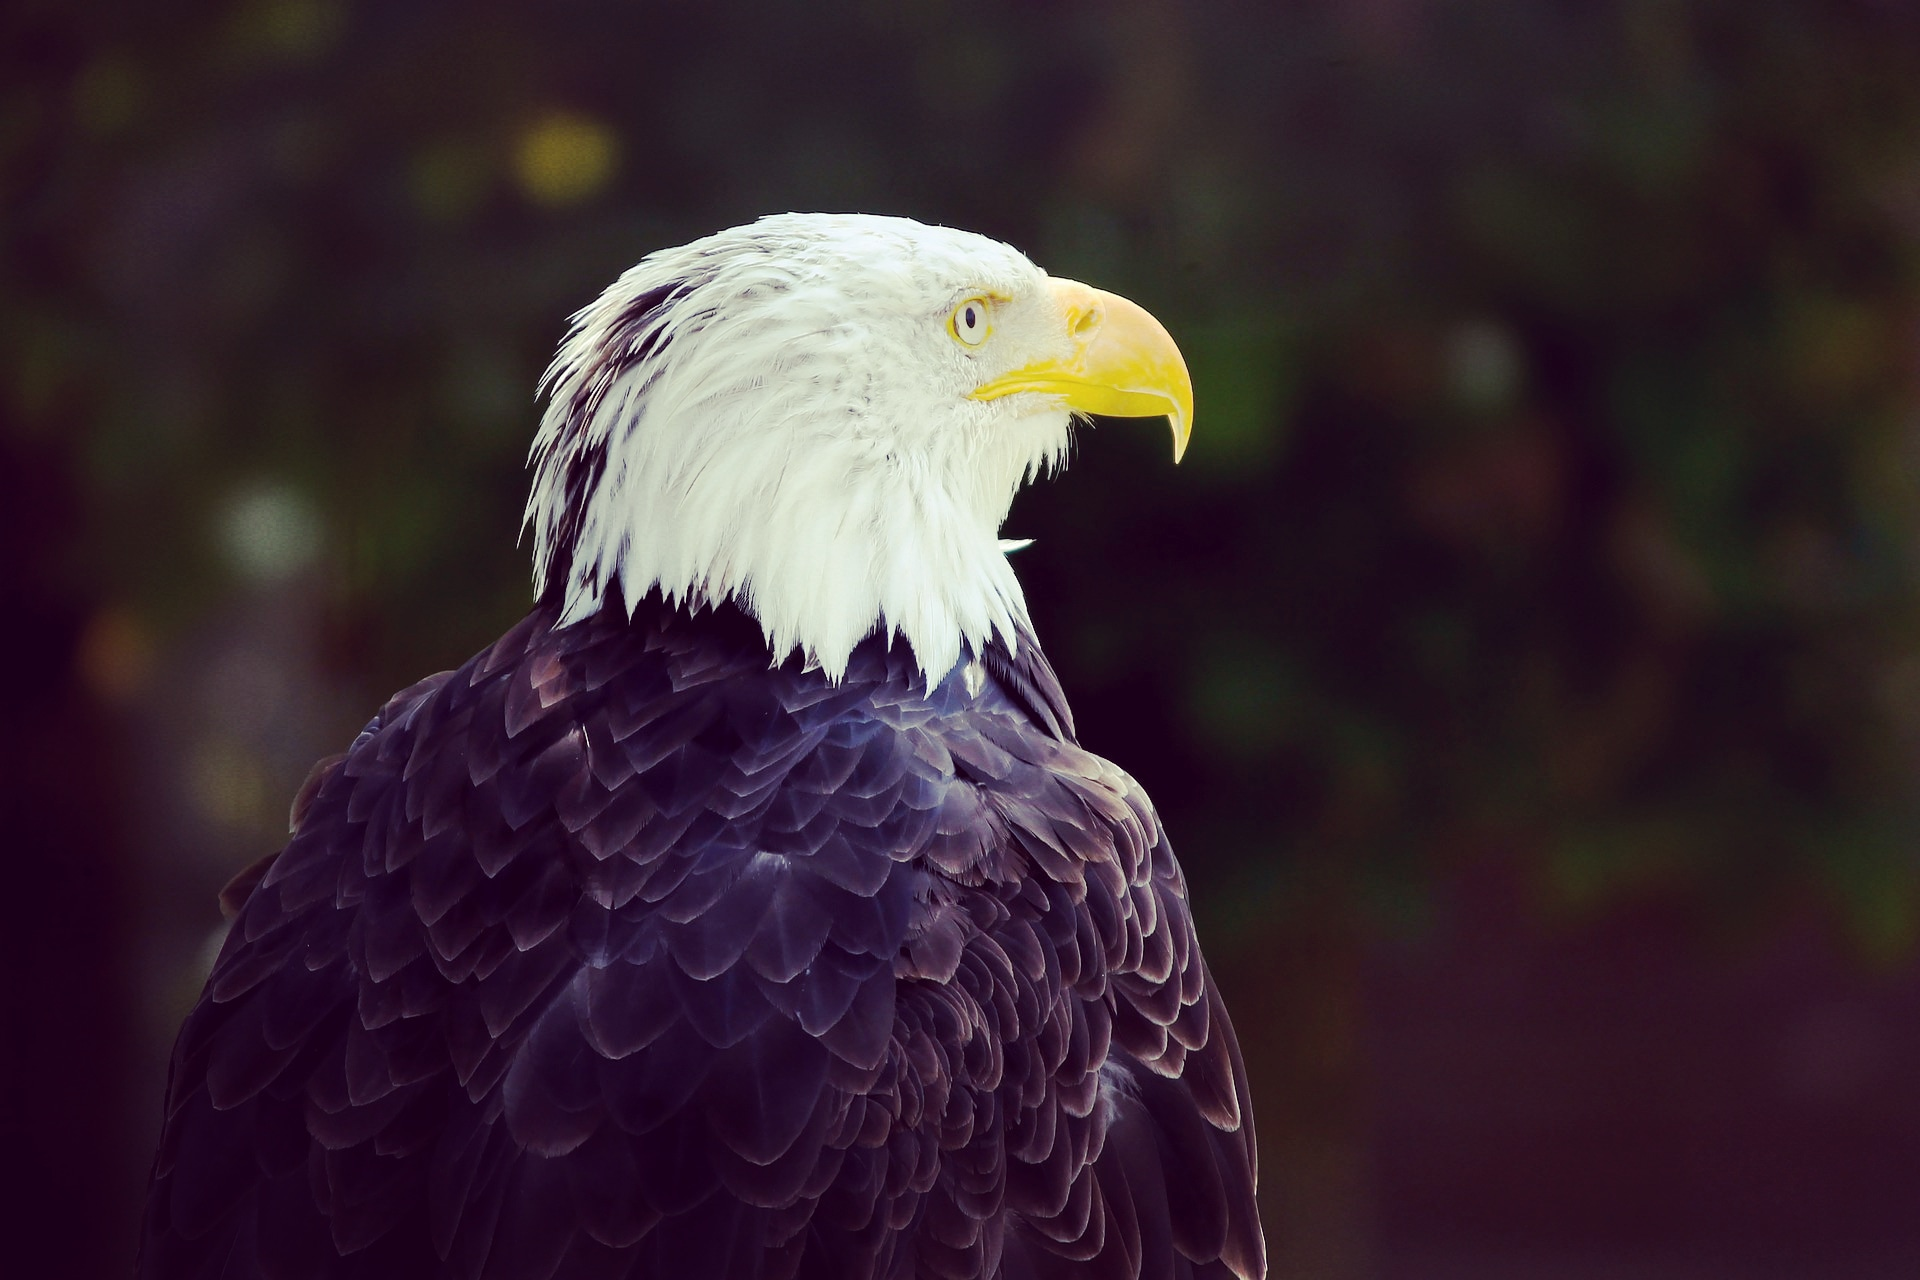
\includegraphics[width=0.4\textwidth]{eagle-amaro.jpg}
  \caption{der Instagramfilter ``Amaro'' auf ein Beispielbild angewandt \cite{res:eagle_image}}
\end{figure}

\para{}
Ein Filter ist eine Region, die deutlich kleiner ist als das verarbeitete Bild
$\ten{B}$, welche über alle Pixel wandert, diese manipuliert und so wieder ein neues Bild
$\tilde{\ten{B}}$ erzeugt.
Mathematisch gesehen handelt es sich bei einem solchen Filter um einen Tensor,
den sogenannten \keyword{Filtertensor} $\ten{F}$ oder auch Faltungstensor (siehe Abb.
\refbox{fig:filter2d}) und Abb. \refbox{fig:filter3d}. Solche Filter sind immer quadratisch, wobei ihre
Zeilen- und Spaltenlänge mit $f$ bezeichnet wird. Dabei ist $f$ immer eine ungerade Zahl, damit ein
Element, das sogenannte \keyword{Zentralelement} (engl.: center element), bezeichnet mit $(\ten{F})_C$,
immer im Zentrum des Filters liegt. \\

\begin{figure}[h!]
  \centering
  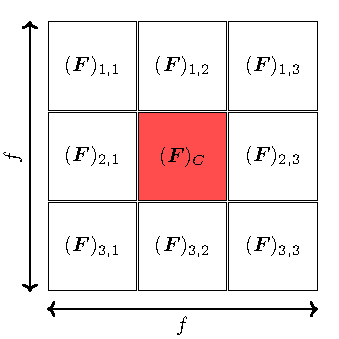
\includegraphics[width=0.3\textwidth]{filter2d.pdf}
  \captionof{figure}{eine 2D-Filtermatrix mit rotem Zentralelement $(\mat{F})_C$}
  \label{fig:filter2d}
\end{figure}
\para{}
Das Verhalten des Filters wird durch seine Tensoreinträge bestimmt.
Die Elemente können so gewählt werden, dass bei Anwendung des Filters auf
ein Bild, dieser bestimmte Features hervorhebt. Solche Features
könnten zum Beispiel Ränder oder Kanten sein, welche akzentuiert werden.
\para{}
Nun wird ein beispielhafter Kantendetektionsfilter betrachtet. Er besitzt die
Filtergrösse $f=3$ und seine Einträge lauten folgendermassen:
\begin{equation*}
  \mat{F}_K =
  \begin{pmatrix}
    -1 & 0 & +1 \\
    -2 & 0 & +2 \\
    -1 & 0 & +1 \\
  \end{pmatrix}
\end{equation*}

Angewendet auf ein schwarz-weisses Bild wird ein neues Bild erzeugt, bei welchem alle erkannten
Kanten weiss eingefärbt werden und die restlichen Bereiche schwarz sind.
Der Filter erkennt dabei jede Stelle als Kante, welche zwei Regionen mit
genug grossem Kontrast voneinander trennt.
In Abbildung \refbox{fig:edge_filter} wurde der erwähnte Kantendetektionsfilter auf ein
Beispielbild angewendet. Links ist das Ursprungsbild und rechts ist das
generierte Bild zu sehen%
\footnote{
  Dieses Bild wurde mithilfe von GIMP (GNU Image Manipulation Program) erzeugt. Dieses
  Programm bietet die Möglichkeit, eine Filtermatrix auf ein Bild anzuwenden.
}.

\begin{figure}[h!]
  \centering
  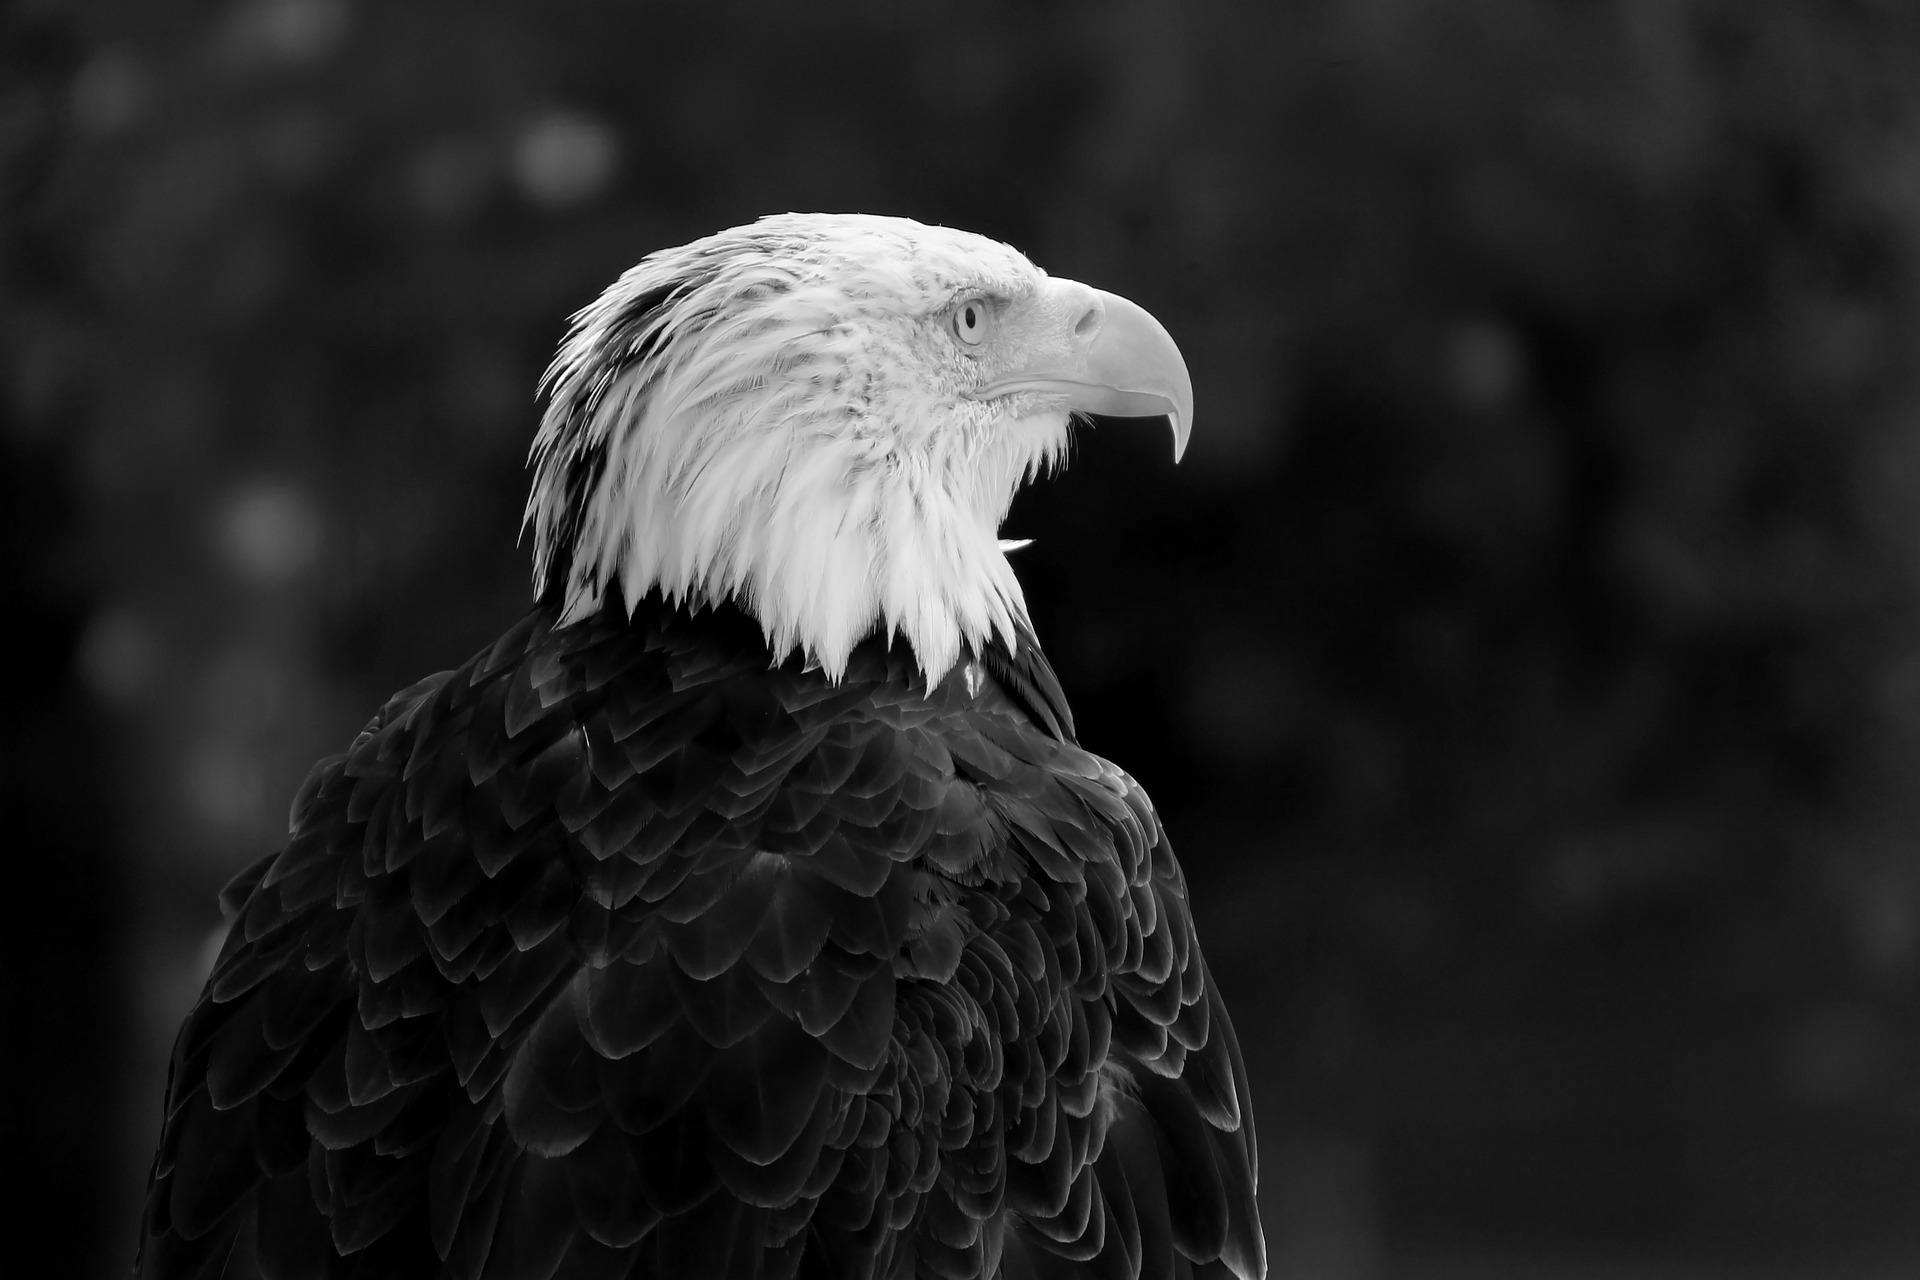
\includegraphics[width=0.4\textwidth]{eagle-gray.jpg}
  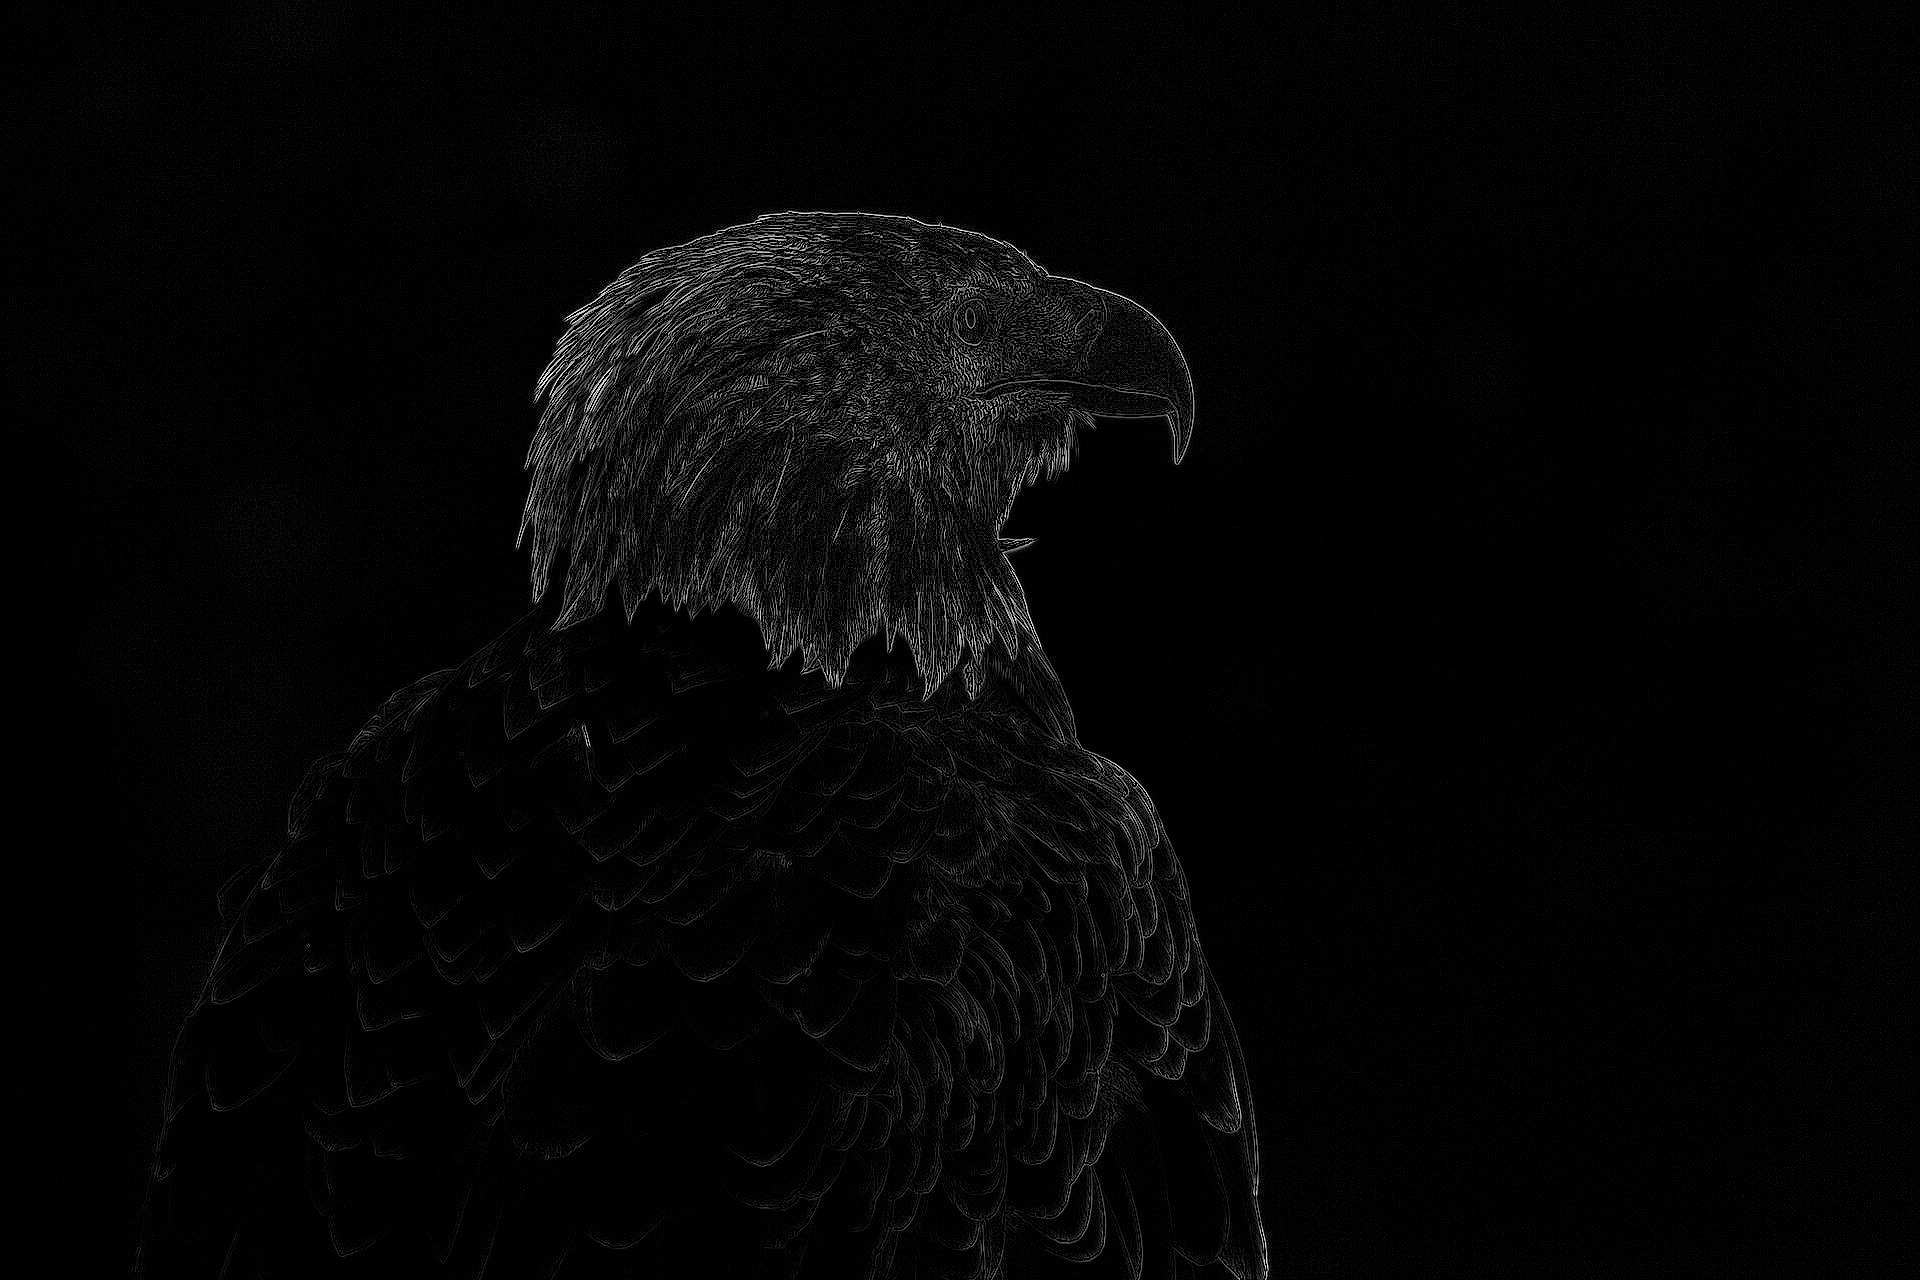
\includegraphics[width=0.4\textwidth]{eagle-gray-filtered.jpg}
  \caption{Kantendetektionfilter angewandt auf Beispielsbild \cite{res:eagle_image}}
  \label{fig:edge_filter}
\end{figure}

\para{}
Quellen: \cite{deeplearning.ai:cnn} \cite{wiki:kernel} \cite{net:gimp_conv}


\subsection{Filter in CNNs}
Aus didaktischen Gründen betrachten wird nun zunächst
nur 2D-Filter, welche sich für graustufige Bilder
$\mat{B} \in \set{R}^{h \times w}$ eignen. Somit ist der hierfür ausgewählte
Filter eine 2D-Matrix, bezeichnet mit $\mat{F} \in \set{R}^{f \times
  f}$. Man bedenke, dass es sich im allgemeinen Fall bei jeder Filtermatrix
um einen 3D-Tensor handelt.
\para{}
Wie bereits dargelegt können Filter genutzt werden, um gewisse
Features eines Bildes hervorzuheben und andere Features zu ignorieren. Dabei
bestimmen die Filtereinträge, welche Features extrahiert werden. Somit besteht
die Aufgabe darin, die richtigen Filtereinträge zu bestimmen, damit die
gewünschten Features erkannt werden und auf den gewünschten Output abgebildet
werden. Naheliegend sollte jetzt der Gedanke sein, die Filtereinträge als die
Modellparameter eines CNNs zu definieren.
Mithilfe von SGD sollen erneut diese Parameter
erlernt werden.
\para{}
Da die Filter die gleiche Funktion haben, wie die Gewichte in einem KNN,
bezeichnet man die Filter in einem CNN mit $\mat{W}$. Die Grösse des Filters
stellt dabei einen Hyperparameter dar.

\begin{equation*}
  \mat{W} = \begin{pmatrix}
    w_{1,1} & \cdots & w_{1,f} \\
    \vdots & \ddots & \vdots \\
    w_{f,1} & \cdots & w_{f,f}
  \end{pmatrix}
\end{equation*}
Somit haben wir erfolgreich das Problem mit der Überzahl an Modellparametern aus
Sektion \refbox{sec:CNN} behoben. Es existieren pro Sicht nur noch $f \times f$
Modellparameter, wobei $f$ oft eine kleine Zahl ist.


\subsection{Filteroperation intuitiv}\label{sec:filteroperation_intuitiv}
Wie wendet man nun einen solchen Filter auf ein Bild an? Um das Prozedere einer
Filteroperation leichter verständlich zu machen, soll es erneut für ein
graustufiges Bild $\mat{B} \in \set{R}^{h \times w}$ erläutert werden. Zu einem
später Zeitpunkt wird auch die Anwendung auf farbige
Bilder erläutert (siehe Sektion \refbox{sec:filteroperation_mathematisch}).
\para{}
Bei einer Filteroperation wendet man einen Filter $\mat{W}$ auf eine Bildmatrix
$\mat{B}$ an und erhält so ein neues Bild $\tilde{\mat{B}}$. Man schreibt dafür:
$\tilde{\mat{B}} = \mat{W} * \mat{B}$.
\para{}
Um nun diese Operation zu erklären, wird als Beispiel eine
2D-Filtermatrix $\mat{W} \in \set{R}^{3 \times 3}$ verwendet, bei welcher
$f = 3$ gewählt wurde.
Wie bereits oben erwähnt, wandert der Filter über das Bild. Dabei befindet
sich der Filter immer über einer Region des Bildes, welche gleich gross ist
wie der Filter selbst (in diesem Fall ($3 \times 3$)). Diese Region des Bildes
bezeichnet man als das \keyword{Rezeptives Feld} des Filters. Man bezeichnet es mit $\hat{\mat{B}}
\in \set{R}^{3 \times 3}$. Somit ist das Rezeptive Feld eine Untermatrix der Obermatrix $\mat{B}$.
\para{}
In diesem Bereich entsprechen den Filtermatrixeinträgen immer eindeutige Bildmatrixeinträge.
Jedem Element des Filters entspricht ein Element des Rezeptiven Feldes. Dem
Zentralelement $(\mat{W})_C$ ist dabei gerade der sogenannte Quellenpixel
(engl.: source pixel) $(\ten{B})_S$ des Bildes zugeordnet. Ihn verwenden wir für eine
Namenskonvention für das Rezeptive Feld. Das Rezeptive Feld wird mit
$\hat{\mat{B}}^{(y,x)}$ bezeichnet, wobei die hochgestellten Indizes $(y,x)$ die Position
des Quellenpixel $(\mat{B})_S$ im Bild $\mat{B}$ angibt.
\para{}
Der Filter beginnt nun oben links über das Bild zu wandern. Somit
hat der Filter zu anfang das Rezeptive Feld $\hat{\mat{B}}^{(2,2)}$, denn der
Filter darf nicht über die Ränder des Bildes hinausragen.
Nun werden die Elemente des Filters mit den Elementen des Rezeptiven Feldes
verrechnet, welche die gleichen Dimensionen besitzen. Dabei wird das
Hadamard-Produkt (das elementweise Produkt, erwähnt in Anhang \refbox{sec:anhang_bp}) der beiden Matrizen miteinander
gebildet. Daraus resultiert eine neue Matrix $\mat{W} \odot
\hat{\mat{B}}^{(2,2)} = \mat{P} \in \set{R}^{3 \times 3}$.
Anschliessend werden alle Elemente der neuen Matrix $\mat{P}$
aufsummiert. Dieser Wert ist dann der Grauwert des ersten Pixels
$(\tilde{\mat{B}})_{1,1}$ des neu entstandenen
Bildes (siehe Gl. \refbox{eq:filter1}). In diesem Sinne stellt der Filter eine
Gewichtung der Nachbarspixel des Ursprungsbild dar, welche
bestimmt, wie die neuen Pixel aussehen.
\\
\begin{equation}\label{eq:filter1}
  (\tilde{\mat{B}})_{1,1} = \Sigma(\mat{P}) = \sum_{y=1}^3 \sum_{x=1}^3 (\mat{P})_{y,x}
\end{equation}
\\
Nun wird der Filter um ein Element nach rechts verschoben und die gleiche
Prozedur angewendet, um den zweiten Pixel zu berechnen. Dies
wird so lange vollzogen, bis eine ganze Zeile der Bildmatrix durchstreift wurde.
Danach wird der Filter wieder ganz nach links verschoben und er bewegt sich ein
Element nach unten. Das geschieht, bis das ganze Bild verrechnet wurde.
Dabei werden die Elemente des ursprünglichen Bildes durchaus mehrfach
verrechnet, da es zu einer Überlappung der vorherigen Position des Filters und
der verschobenen Position kommt.
\para{}
\begin{figure}[h!]
  \centering
  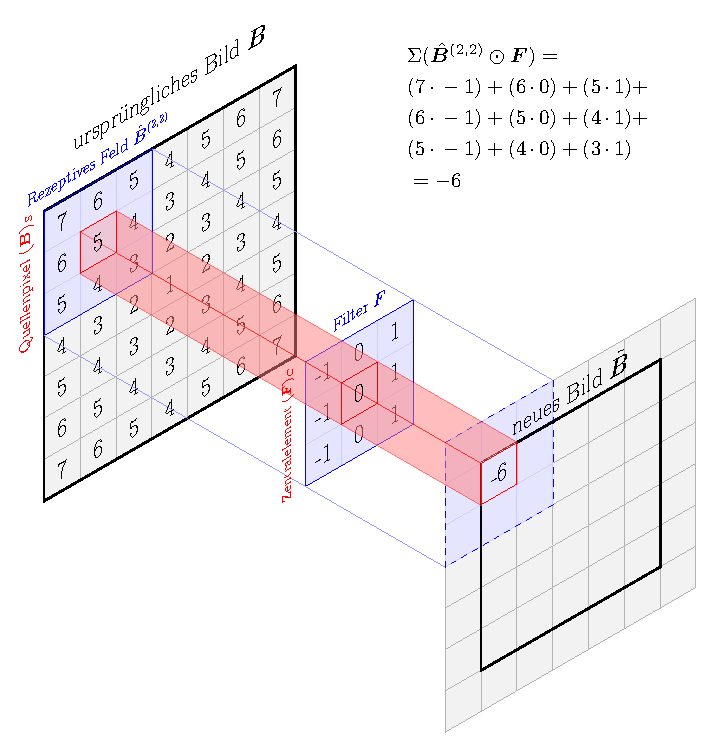
\includegraphics[width=0.6\textwidth]{conv.pdf}
  \caption{Schema, wie ein Filter über ein Bild läuft}
  \label{fig:filteroperation}
\end{figure}
\para{}
Es ist zu bemerken, dass das neue Bild $\tilde{\mat{B}} \in \set{R}^{(h-2) \times (w-2)}$ nicht mehr die gleichen Masse
aufweist wie das Ursprungsbild $\mat{B} \in \set{R}^{h \times w}$. Das liegt daran, dass pro
Lage des Filters jeweils nur ein Pixel des neuen Bildes entsteht. Man kann
sich vorstellen, dass an der Position des Quellenpixels jeweils ein neuer
Pixel generiert wird. Jedoch muss der Filter immer eine vollständige Region als
Rezeptives Feld besitzen. Dadurch kommt das Zentralelement nie auf die Ränder des
Bildes zu liegen, wodurch sie entfallen.
\para{}
Dieses ganze Verfahren der Filteroperation ist anschaulich in Abbildung
\refbox{fig:filteroperation} dargestellt.
\para{}
Quellen: \cite{deeplearning.ai:cnn} \cite{wiki:convolution}

\subsection{Filteroperationen als diskrete Faltungen}\label{sec:filteroperation_mathematisch}
Eigentlich handelt es sich bei der Anwendung eines Filters auf ein Bild um
eine spezifische mathematische Operation: eine \keyword{diskrete Faltung}%
\footnote{
  Streng genommen wird in CNNs nicht eine diskrete Faltung durchgeführt, sondern
  eine sogenannte \keyword{Kreuzkorrelation}. Der Unterschied besteht darin, dass bei einer
  Kreuzkorrelation die Faltungsmatrix nicht horizontal und vertikal
  gespiegelt wird. Dies, im Gegensatz zu der eigentlichen Faltung, bei welcher
  diese Spiegelung stattfindet. Jedoch wird
  begrifflich das Wort Faltung für beide Operationen verwendet. Im Rahmen dieser
  Arbeit ist mit dem Wort Faltung immer die Kreuzkorrelation gemeint.
} (engl.: \keyword{convolution}).

Daher rührt auch der Name des Convolutional Neural Networks.
Da die Faltung als mathematische Operation relativ kompliziert ist, wird sie im
Rahmen dieser Arbeit nicht in vollem Umfang behandelt.
Ihre Bedeutung soll auf die Faltung von Filtern beschränkt werden.
\para{}
Mithilfe der Faltungsoperation können die Schritte aus Sektion
\refbox{sec:filteroperation_intuitiv} zusammengefasst werden.
Bei der Filteroperation handelt es sich nämlich um eine diskrete Faltung des
Filtertensors $\ten{W}$ über den Bildtensor $\ten{B}$. Somit kann
folgende Formel verwendet werden, um einen Pixel $\tilde{\mat{B}}_{y,x}$ des neuen Bildes zu berechnen.
\\
\begin{equation}
  (\tilde{\mat{B}})_{y,x} = (\mat{W} * \mat{B})_{y,x} = \sum_{v=1}^{f} \sum_{u=1}^{f} (\mat{W})_{v,u}(\mat{B})_{y+v-1,x+u-1}
\end{equation}
\para{}
\begin{examplebox}{Faltung Beispielrechnung}
  Es folgt nun eine Beispielrechnung für eine Faltungsoperation zweier Matrizen.
  Diese Matrizen haben folgende Einträge:
  \\
  \begin{equation*}
    \mat{B} =
    \begin{pmatrix}
      10 & 10 & 10 & 0 & 0 & 0 \\
      10 & 10 & 10 & 0 & 0 & 0 \\
      10 & 10 & 10 & 0 & 0 & 0 \\
      10 & 10 & 10 & 0 & 0 & 0 \\
      10 & 10 & 10 & 0 & 0 & 0 \\
      10 & 10 & 10 & 0 & 0 & 0 \\
    \end{pmatrix}
    \text{ und } \mat{W} =
    \begin{pmatrix}
      1 & 0 & -1 \\
      1 & 0 & -1 \\
      1 & 0 & -1 \\
    \end{pmatrix}
  \end{equation*}
  \\
  Um den ersten Pixel $(\tilde{\mat{B}})_{1,1}$ des Resultats zu erhalten, führen wir folgende Rechnung durch:
  \begin{gather*}
    (\tilde{\mat{B}})_{1,1} = (\mat{W} * \mat{B})_{1,1} = \sum_{v=1}^{f} \sum_{u=1}^{f} (\mat{W})_{u,v} (\mat{B})_{u,v} \\
                           = (10 \cdot 1) + (10 \cdot 0) + (10 \cdot -1) + (10 \cdot 1) + (10 \cdot 0) + (10 \cdot -1) + (10 \cdot 1) + (10 \cdot 0) + (10 \cdot -1) \\
                           = 0
  \end{gather*}

  Das Gesamtergebnis lautet dann:
  \begin{equation*}
    \tilde{\mat{B}} = \mat{W} * \mat{B} =
    \begin{pmatrix}
      0 & 30 & 30 & 0 \\
      0 & 30 & 30 & 0 \\
      0 & 30 & 30 & 0 \\
      0 & 30 & 30 & 0 \\
    \end{pmatrix}
  \end{equation*}
\end{examplebox}
\para{}
Für farbige Bilder ist das Vorgehen ähnlich. Es werden nun
Tensoren dritten Ranges anstatt von Tensoren zweiten Ranges verwendet.
Betrachten wird der allgemeinen Bildtensor $\ten{B} \in \set{R}^{h \times w
  \times c}$, wobei $c$ die Anzahl Farbkomponenten (engl.: channels) ist.
Nun benutzt man einen Filter $\ten{W} \in \set{R}^{f \times f \times c}$ mit beliebiger Grösse
$f$, aber mit der gleichen Tiefe $c$, wie das Ursprungsbild $\ten{B}$.
Dadurch muss der Filter nicht entlang der Tiefe des Bildes wandern, weil er
die gleiche Tiefe aufweist. Das hat zur Folge, dass das verarbeitete
Bild $\tilde{\mat{B}}$ immer eine Matrix ist.
Die allgemeine Filtergleichung lautet:
\\
\begin{equation}\tag{FO}
  (\tilde{\mat{B}})_{y,x} = (\ten{W} * \ten{B})_{y,x} = \sum_{v=1}^{f} \sum_{u=1}^{f} \sum_{w=1}^c (\ten{W})_{v,u,w} (\ten{B})_{x+u-1,y+v-1,w}
\end{equation}
\para{}
\begin{figure}[h!]
  \centering
  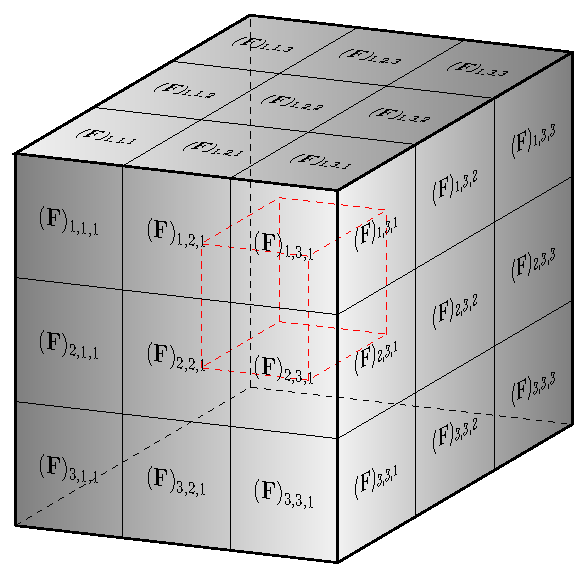
\includegraphics[width=0.4\textwidth]{filter3d.pdf}
  \captionof{figure}{ein 3D-Filtertensor mit rotem Zentralelement $(\ten{F})_C$}
  \label{fig:filter3d}
\end{figure}

\para{}
Quellen: \cite{Goodfellow-et-al-2016} \cite{deeplearning.ai:cnn} \cite{wiki:cnn}

\subsection{Mehrere Filter}
Eine Filteroperation ist nicht auf einen einzigen Filter beschränkt. Es können
mehrere Filter auf das gleiche Ausgangsbild angewendet werden und zusammen ein
Endbild erzeugen.
\para{}
Die Anzahl Filter werden mit $c$ bezeichnet.
Nun wird pro Filter $\ten{W}_i$ eine Faltung über das Ursprungsbild $\ten{W}$ gemacht, wobei
jede Faltung eine neue Matrix $\tilde{\mat{B}}_i = \ten{W}_i * \ten{B}$ liefert.
Dabei ist $i$ der Index des Filters. All diese gefalteten Bilder
$\tilde{\mat{B}}_i$ sind zwei-dimensionale Matrizen, unabhängig davon, wie viele
Komponenten das Ursprungsbild hatte. Aus diesem Grund können die einzelnen
Matrizen $\tilde{\mat{B}}_i$ aufeinander gelegt werden und somit einen grossen 3D-Endtensor
$\tilde{\ten{B}}$ bilden.
Hierfür müssen alle Filter $\ten{W}_i$ gleich gross sein.
Die Tiefe des neuen Bildes $\tilde{\ten{B}}$ ist jetzt gerade die Anzahl Filter $c$.
Schon vorher wurde die Tiefe des Bildes (bzw. die Anzahl
Farbkomponenten) mit $c$ bezeichnet. Somit steht $c$ sowohl die Anzahl Filter
einer Schicht, wie auch für die Tiefe des verarbeiteten Bildes.

\para{}
Quellen: \cite{Goodfellow-et-al-2016} \cite{deeplearning.ai:cnn}

\subsection{Padding}
Wie bereits erwähnt schrumpfen die Bilder (an den Rändern), wenn man einen Filter auf sie anwendet.
Zur Erinnerung: Dies liegt daran, dass pro Lage des Zentralelements jeweils nur ein Pixel
des neuen Bildes entsteht. Das Zentralelement kommt jedoch nicht auf allen
Ursprungspixeln zu liegen. Auf diese Weise fallen die Ränder weg. Der Umfang des
Wegfalls hängt von der Filtergrösse $f$ ab. Folgende Formel gilt für die
neue Grösse $n_1$ des Bildes, berechnet anhand der alten Grösse $n_0$. $n$ bezeichnet
eine der zwei Seitenlängen.
\begin{equation}
  n_1 = n_0 - f + 1
\end{equation}

Das Problem hierbei ist, dass nach einigen Faltungen das Bild extrem geschrumpft
ist und im Grenzfall kleiner als der Filter wird. Das darf natürlich nicht
passieren. Zusätzlich kommt es zu einem relativen Informationsverlust an den
Rändern, im Vergleich zum Rest des Bildes. Dies rührt daher,
das es im Innern des Bildes zu mehr Überlappungen der Filterlagen kommt und dies
bei den Rändern seltener auftritt.
\para{}
Diese unerwünschten Phänomene lassen sich mit sogenanntem \keyword{Padding} beheben. Padding ist ein
Vorgang, welcher vor der eigentlichen Faltung stattfindet. Dabei werden
zusätzliche Ränder (Zeilen und Spalten) an das Ursprungsbild angebracht. Der
)Tensor wird der Länge und der Breite (und nicht der Tiefe) entlang an den
Enden erweitert. Die neuen Elemente werden dabei auf den Wert $0$ gesetzt.

\begin{figure}[h!]
  \centering
  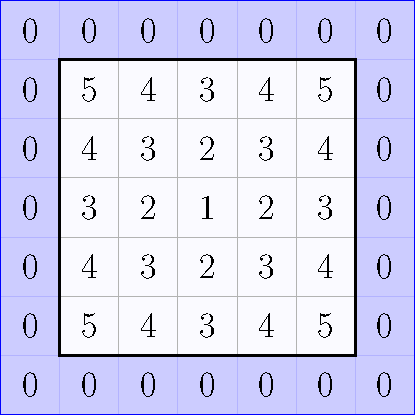
\includegraphics[width=0.2\textwidth]{padding.pdf}
  \caption{Padding $p=1$ in blau}
\end{figure}

Das Padding $p$ ist eine Zahl, welche angibt, wie viele Elemente an allen Rändern
hinzugefügt werden. Padding $p = 1$ bedeutet, dass an allen Kanten jeweils eine
Reihe bzw. Spalte hinzugefügt wird.
Begrifflich unterscheidet man zwischen zwei Arten von Padding:
\begin{itemize}
\item{\keyword{Valid-Padding}: Es werden keine zusätzlichen Elemente angebracht. $p$ ist also 0.}
\item{\keyword{Same-Padding}: Es werden so viele Reihen und Spalten angebracht, dass
    die Grösse des Bildes nach der Faltung unverändert bleibt.}
\end{itemize}
\para{}
Um Same-Padding durchzuführen, muss $p$ so gewählt werden, dass es den Wegfall durch
die Filteroperation gerade kompensiert. Da die Bilder durch das Padding der Länge und
Breite nach jeweils um zwei $p$ verlängert wird, erhält man den Ausdruck $n_1 =
n_0 - f + 1 + 2p$. Wenn diese Formel nach $p$ auflöst,
erhält man folgende Formel für das Wählen des Same-Paddings $p$.
\\
\begin{equation}
  p = \frac{f-1}{2}
\end{equation}

\para{}
Quellen: \cite{deeplearning.ai:cnn}

\subsection{Stride}
Bis jetzt wurde bei den Filterfaltungen der Filter pro Verschiebung immer nur
um einen Pixel bewegt. Dies ist nicht zwingend. Grundsätzlich können Filter auch
mit anderen Schrittgrössen verschoben werden.
Diese Schrittgrösse bezeichnet
man als \keyword{Stride} $s$. Falls $s = 2$ gewählt wird, bedeutet das, dass der
Filter sich pro Hadamard-Produkt um zwei Elemente verschiebt. Somit wurde eine
Position übersprungen. Dies hat zur Folge, dass das neue Bild
deutlich kleiner wird, denn das Zentralelement überspringt somit auch
diese Felder und bildet so deutlich weniger Pixel.
\para{}
\begin{figure}[h!]
  \centering
  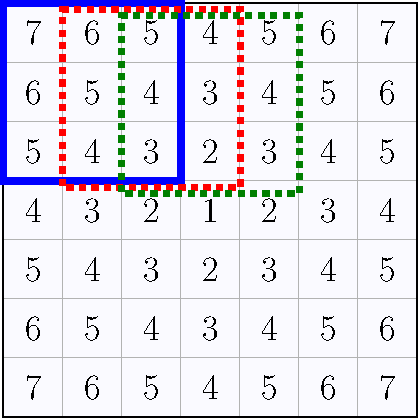
\includegraphics[width=0.2\textwidth]{stride.pdf}
  \caption{Abbildung zum Stride: Ausgangsposition in blau, nächste Position mit
    $s=1$ in rot, nächste Position mit $s=2$ in grün}
\end{figure}
\para{}
Folgende Formel beschreibt die Dimensionen des neuen Bildes unter
Berücksichtigung der Filtergrösse $f$, dem Padding $p$ und dem Stride $s$.
\\
\begin{equation}
  n_1 = \frac{n_0 + 2p - f}{s} + 1
\end{equation}

Quellen: \cite{deeplearning.ai:cnn}

\subsection{Vorzüge von Filtern}
Es stellt sich nun die Frage, weshalb sich Filter für Maschinelles
Lernen mit Bildern besonders eignen.
Wie bereits erwähnt besteht die Aufgabe der Filter darin, bestimmte Features
eines Bildes hervorzuheben und die restlichen auszublenden. Die gleiche
Aufgabe erfüllen die Neuronen in einem KNN. Auch sie sollen Features der
Inputdaten erlernen, wobei gewisse Neuronen auf gewisse Features reagieren.
Weshalb verwendet man also nicht einfach KNNs (abgesehen
von dem Problem mit der grossen Menge an Modellparametern, siehe Sektion
\refbox{sec:CNN_parameter_problem})?
\para{}
Man muss erkennen, dass sich Bilddaten deutlich von sonstigen Daten unterscheiden.
Bildfeatures bzw. Pixel sind nur im Kontext ihrer Nachbarn relevant. Denn
ein Pixel ist erst dann eine Kante oder eine Ecke, wenn er zwei verschiedene
Farbregionen voneinander trennt. Oder ein Gegenstand wird erst durch eine ganze Anzahl
von Pixeln und deren relative Position zueinander charakterisiert.
Man bezeichnet diesen Umstand als \keyword{lokalisierte Features}.
\para{}
Des Weiteren sind Bildausschnitte nicht immer gleich
ausgerichtet. Wenn man ein Gesicht auf einem Bild erkennen möchte, sollte es aber
keine Rolle spielen, wo es sich auf dem Bild befindet, welche Grösse es
hat und welche Ausrichtung es aufweist. Um diese Eigenschaften irrelevant für das
Modell zu machen, muss es gewisse \keyword{Invarianzen} erfüllen.
\para{}
Der Wesenszug, welche CNNs für lokalisierte Features und
Invarianzen geeignet macht, bezeichnet man als \keyword{Parameter-Sharing}.
Er bezeichnet den Umstand, dass auf
mehrere oder alle Features die gleichen Modellparameter wirken. Bei CNNs wird
dies durch die Bewegung des Filters bzw. seiner Einträge über (fast) alle
Pixel bewerkstelligt. Somit ist
es egal, wo und wie sich die lokalisierten Features befinden. Dies führt dann zu
den gewünschten Invarianzen: Translations-, Rotations- und
Helligkeitsinvarianz.
\para{}
Ein weiterer Vorteil des Parameter-Sharing ist, dass die Inputbilder
beliebige Dimensionen besitzen können, da die Filter ihre Bewegung lediglich an
die Grösse des Bildes anpassen müssen.
\para{}
Quellen: \cite{deeplearning.ai:cnn}

\subsection{Convolutional-Schicht}
Nun soll zusammengeführt werden, was soeben über Filter erläutert
wurde, um die Convolutional-Schicht zu definieren.
\para{}
Die Convolutional-Schicht $l$ beginnt mit ihrem Input, also den
Aktivierungen $\ten{A}^{l-1} \in \set{R}^{h^l \times w^l \times c^l}$, welche die vorherige Schicht ($l-1$) produziert hat.
Falls es sich um die erste Schicht handelt, erhält sie den Input $\ten{X}$ des Netzes.
\para{}
Die Schicht besitzt $c^l$ Varianten an Filtern $\ten{W}^l_i \in
\set{R}^{f^l \times f^l \times c^{l-1}}$, wobei $i$ der Index ist. Diese Filter haben alle die gleichen
Eigenschaften bezüglich: der Grösse $f^l$, der Tiefe $c^{l-1}$, dem Padding
$p^l$ und dem Stride $s^l$. Sie unterscheiden sich nur in den Modellparametern.
\\
\begin{equation*}
  \ten{W}^l_i =
  \begin{bmatrix}
    \begin{pmatrix}
      w_{i\,|\,1,1,1}^l & \cdots & w_{i\,|\,1,f,1}^l \\
      \vdots & \ddots & \vdots \\
      w_{i\,|\,f,1,1}^l & \cdots & w_{i\,|\,f,f,1}^l
    \end{pmatrix}
    & \cdots &
    \begin{pmatrix}
      w_{i\,|\,1,1,c^l}^l & \cdots & w_{i\,|\,1,f,c^l}^l \\
      \vdots & \ddots & \vdots \\
      w_{i\,|\,f,1,c^l}^l & \cdots & w_{i\,|\,f,f,c^l}^l
    \end{pmatrix}
  \end{bmatrix}
\end{equation*}
\\
Nun wird jeder Filter $\ten{W}_i^l$ einzeln über das Bild
$\ten{A}^l$ gefaltet, wodurch mehrere neue 2D-Bilder $\tilde{\mat{A}}_i^l$ entstehen.
\\
\begin{equation}
  \tilde{\mat{A}}_i^l = \ten{W}_i^l * \ten{A}^l
\end{equation}
\\
Die Faltung berechnet sich aus folgender Gleichung:
\\
\begin{equation}\tag{FO}
  (\tilde{\mat{A}}_i)_{y,x}^l = (\ten{W}_i^l * \ten{A}^l)_{y,x} = \sum_{v=1}^{f} \sum_{u=1}^{f} \sum_{w=1}^c (\ten{W}^l_i)_{v,u,w} (\ten{A}^l)_{x+v-1,y+u-1,w}
\end{equation}
\\
Jede dieser Matrizen ist ein Querschnitt $\tilde{\mat{A}}^l_{:,:,i}$ entlang der
Tiefe des neuen 3D-Tensors $\tilde{\ten{A}}^l \in \set{R}^{h^{l+1} \times w^{l+1} \times c^l}$.
Hierbei ist die Tiefe $c^l$ gerade die Anzahl der Filter $c^l$. Die Höhe
$h^{l+1}$ und die Breite $w^{l+1}$ werden jeweils gemäss nachstehender Formel berechnet,
anhand der Höhe $h^l$ und der Breite $w^l$ des Ausgangsbildes:
\\
\begin{equation}
  n^{l+1} = \frac{n^l + 2p^l - f^l}{s^l} + 1
\end{equation}
\\
Da die Faltungsoperation linear ist, wird wiederum eine
nicht-lineare Aktivierungsfunktion benötigt, um das Modell zu befähigen, nicht-lineare Probleme
zu lösen.
Deshalb wird in einem letzten Schritt die vektorisierte Aktivierungsfunktion
$\vecf{\varphi}$ auf den Tensor $\tilde{\mat{A}}^l$ angewendet. So ergibt sich die
neue Aktivierung $\ten{A}^{l+1}$ der nächsten Schicht. Empirisch lässt sich nachweisen,
dass sich für CNNs die ReLU-Aktivierungsfunktion aus Sektion \refbox{sec:ReLU} besser eignet als die
Sigmoidfunktion. Deshalb wird in der Regel die ReLU-Funktion für CNNs verwendet.
\begin{equation}
  \ten{A}^{l+1} = \vecf{\varphi}[\tilde{\ten{A}}^l]
\end{equation}
\para{}
Quellen: \cite{wiki:cnn} \cite{deeplearning.ai:cnn} \cite{Goodfellow-et-al-2016} \cite{Nielsen}

\section{Dimensionalitätskontrolle}\label{sec:dimensionalitätskontrolle}
Beim Anwenden einer Convolutional Schicht gehen Informationen verloren, da nur
die relevanten Features hervorgehoben werden und der Rest verworfen wird. Jedoch
schrumpft das Bild entweder gar nicht (bei Same-Padding) oder es schrumpft nur
vergleichsweise leicht (bei Valid-Padding). Dies ist ein Problem, da die Information in
deutlich weniger Pixeln bzw. Tensorelementen codiert werden könnte. In der Konsequenz
zeigt sich ein unnötig hoher Ressourcenverbrauch und eine erhöhte Gefahr für
Overfitting (siehe Sektion \refbox{sec:overfitting}). Um diesem Effekt
entgegenzuwirken, gibt es einerseits sogenannte
\keyword{Pooling-Schichten} und als Gegenstück dazu
\keyword{Upsampling-Schichten}. Ersteres wird verwendet, um die Dimensionalität
der Bilder zu vermindern und Letzteres, um die Dimensionalität der Bilder zu
erweitern. Somit ermöglichen diese Schichten eine kontrollierte Art, (im Gegensatz zum
Padding) die Dimensionalität willentlich zu bestimmen. Diese Fähigkeit ist
essenziell, um in Sektion \refbox{sec:convolutional_autoencoder} die Topologie
eines Convolutional Autoencoders zu realisieren.

\subsection{Pooling-Schicht}
Die Pooling-Schicht verringert die Dimensionalität durch das Zusammenfassen eines Feldes
von Tensorelementen zu einem einzigen Tensorelement.
Dabei wandert das Feld nur entlang der Länge und Breite des Bildes und
nicht etwa entlang der Tiefe. Dies bedeutet, dass das Pooling auf jede Farbkomponente
einzeln angewendet wird, wodurch sich die Tiefe des Bildes nicht ändert.
\para{}
Für die Beschreibung einer Pooling-Schicht finden die gleichen Begriffe
Anwendung wie bei der Convolutional-Schicht und den Filtern.
Die Grösse des Elementefeldes, welches zusammengefasst wird, bezeichnet man analog zur
Filtergrösse mit $f^l$. Das Stride $s^l$ bezeichnet auch beim Pooling, wie
gross die Schrittgrösse beim Verschieben des Feldes ist. Meistens wählt man den
Stride $s^l$ gerade gleich der Feldgrösse $f^l$, damit alle Pixel
zusammengefasst werden. Kleiner als $f^l$ kann $s^l$ nicht gewählt werden.
\para{}
Man unterscheidet zwischen zwei Arten von Pooling:
\begin{itemize}
\item{\keyword{Average-Pooling}: Das Elementefeld wird zusammengefasst, indem
    das arithmetische Mittel der Elemente gebildet wird.}
\item{\keyword{Max-Pooling}: Das Elementefeld wird zusammengefasst, indem das
    Element mit dem höchsten Wert beibehalten wird und die anderen verworfen werden.}
\end{itemize}
In der Praxis verwendet man eigentlich nur Max-Pooling, da es deutlich bessere
Resultate erzielt.
\para{}
\begin{examplebox}{MaxPooling Beispiel}
  Es sei eine MaxPooling-Schicht gewählt mit $f^l = 2$ und $s^l = 2$.
  Diese fasst also jedes $(2 \times 2)$-Feld zu einem Element zusammen. Da aus
  vier Elementen jeweils eines wird, entspricht dies einer Informationsreduktion
  von 75\%.
  \para{}
  \begin{equation*}
    \begin{pmatrix}
      5 & 2 & 4 & 3 \\
      8 & 9 & 5 & 1 \\
      3 & 8 & 6 & 7 \\
      8 & 1 & 4 & 2 \\
    \end{pmatrix}
    \to_{\text{MaxPool}}
    \begin{pmatrix}
      9 & 5 \\
      8 & 7 \\
    \end{pmatrix}
  \end{equation*}
\end{examplebox}
\para{}
Es ist festzuhalten, dass eine Pooling-Schicht keinerlei Modellparameter
besitzt. Somit gibt es nichts zu trainieren. Sie besitzt lediglich einige
Hyperparameter, wie die Feldgrösse $f^l$ und den Stride $s^l$.
\para{}
Um zu berechnen, was die neuen Dimensionen des Bildes nach dem Pooling sind, gelten die
gleichen Formeln wie für die Filteroperationen:
\\
\begin{equation}
  n_1 = \frac{n_0 - f}{s} + 1
\end{equation}
\\
\para{}
Quellen: \cite{deeplearning.ai:cnn} \cite{Goodfellow-et-al-2016}

\subsection{Upsampling-Schicht}
Die Upsampling-Schicht bildet das Gegenstück zur Pooling-Schicht, da sie die
Dimensionalität des Bildes erhöht. Auf den ersten Blick erscheint unklar,
weshalb man die Dimensionalität erhöhen will, da die eigentliche
Motivation dieser Schichten in der Verhinderung von Overfitting besteht. Jedoch
sollte mit dem Kapitel \refbox{sec:autoencoder} klar werden, weshalb solche Schichten
höheren Nutzen haben können.
\para{}
Man verwendet auch hier wieder den Begriff der Feldgrösse $f^l$. Dieses Mal
beschreibt der Wert, wie stark das Bild hochskaliert wird. Beim Upsampling
wird ein Element zu einem $(f^l \times f^l)$-Feld hochgerechnet und erweitert so die
Dimensionalität.
\para{}
Es stellt sich die Frage, welche Werte das neue Feld erhält.
Dafür ist eine Interpolationsart zu wählen.
Zwei Arten sind besonders verbreitet:
\begin{itemize}
\item{\keyword{Bilineare Interpolation}}
\item{\keyword{Nächste-Nachbar-Interpolation} (engl.: nearest-neighbor-interpolation)}
\end{itemize}
Hier soll nur die Nächste-Nachbar-Interpolation betrachten werden. Sie ist
vergleichsweise trivial, denn alle neuen Feldelemente nehmen einfach den Wert des alten
Elements an. Der Wert wird auf diese Weise vermehrt.
\para{}
Quellen: \cite{deeplearning.ai:cnn} \cite{Goodfellow-et-al-2016}

\pagebreak
\chapter{Autoencoder}\label{sec:autoencoder}
In Kapitel drei wurde die Architektur eines Convolutional Neural Networks dargelegt.
Nun soll eine weitere Architektur erörtert werden, welche das letzte Bindeglied zur
praktischen Programmierung eines Convolutional-Denoising-Autoencoder verkörpert.
Dieses ist notwendig, um die theoretische Funktionsweise eines Autoencoders zu verstehen.
Zielsetzung ist, den Autoencoder mit dem Convolutional
Neural Network zu fusionieren, um auf diese Weise einen
Convolutional-Autoencoder zu erhalten. Zu
guter Letzt soll dann noch eine Anwendung eines solchen
Convolutional-Autoencoder betrachtet werden, in der Form eines Denoiser.
\para{}
\bigskip
Ein \keyword{Autoencoder} ist eine Architektur, welche ein KNN nicht
bezüglich der Schichtenarten, sondern auf der Ebene der Netzform beschreibt.
Die Aufgabe eines Autoencoders besteht darin, eine neue Repräsentation einer Datenmenge
zu erlernen. Diese neuartige Darstellung soll mit weniger Daten möglichst die gleiche
Information codieren. Somit entwickelt das Modell eine \keyword{effiziente
  Daten-Codierung} für einen Datensatz. Dadurch kann er zur
\keyword{Dimensionalitätsreduktion} verwendet werden.
Neben dieser neuen Repräsentation erlernt das Netzwerk darüber hinaus, wie es
aus dieser Codierung wieder die Ursprungsdaten reproduzieren kann.
\para{}
Autoencoder gehören nicht dem klassischen überwachtem Lernen an. Streng genommen
zählen sie zum unüberwachtem Lernen, da in den Trainingsdaten keine Labels
enthalten sein müssen. Jedoch gilt das gleiche Vorgehen, wie bei Überwachtem Lernen.
Das Netzwerk wird nämlich ebenfalls darauf trainiert, gewisse gewünschte Outputs
zu liefern. Nur sind in diesem Fall die ``Labels'' gleich den Features!
\para{}
Quellen: \cite{book:autoencoder}

\section{Topologie}
Ein Autoencoder besteht ebenso wie das klassische KNN aus Neuronen.
Wie bereits erwähnt sind die ``Labels'' eines Autoencoders gleich
den Features. Somit versucht ein Autoencoder, die Werte der Inputneuronen
möglichst exakt in die Outputneuronen zu kopieren.
Diese Operation wäre an sich ziemlich bedeutungslos, da mit den
Daten nichts passiert. Das Netzwerk würde lediglich erlernen, eine
Identitätsfunktion zu imitieren.
Aus diesem Grund muss man gewisse Einschränkungen einführen. Diese bringen das Netzwerk dazu,
interessante Methoden zu entwickeln, um die Features \textit{approximativ} zu rekonstruieren.
\para{}
Die angesprochene Einschränkung besteht darin, dass dem Autoencoder nicht
beliebig viel Kapazität für die Codierung der Features gewährt wird.
Es stehen dem Netzwerk nur wenige Zahlenwerte zur Verfügung, um die Features
in der neuen Repräsentation zwischenzuspeichern, bevor sie wieder in die
ursprüngliche Form zurück transformiert werden.
Die Kapazitätseinschränkung wird durch die Topologie des Autoencoders bezweckt.
\para{}
\bigskip
Der einfachste Autoencoder besteht aus drei Schichten, welche sich wie folgt
gliedern lassen:
\begin{itemize}
\item{eine Inputschicht mit $d$ Neuronen}
\item{eine Zwischenschicht mit $p$ Neuonen, bezeichnet als \keyword{Flaschenhals}}
\item{eine Outputschicht mit $d$ Neuronen}
\end{itemize}
In Abbildung \refbox{fig:basic_autoencoder} ist
ein beispielhafter Autoencoder abgebildet, mit $d = 5$ Features und einem
Flaschenhals der Grösse $p = 2$.
\begin{figure}[h!]
  \centering
  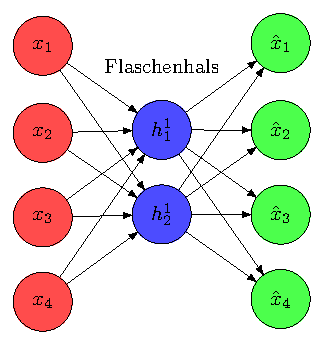
\includegraphics[height=0.3\textwidth]{ae1.pdf}
  \caption{Schichten eines kurzen Autoencoders}
  \label{fig:basic_autoencoder}
\end{figure}
\para{}
Die Inputschicht enthält die Features $\vec{x} \in \set{R}^d$. Dagegen enthält die Outputschicht
die \keyword{Rekonstruktionen} der Features, welche wir mit $\vec{\hat{x}} \in \set{R}^d$
bezeichnen. Als logische Konsequenz müssen die beiden Schichten die gleiche
Anzahl $d$ an Neuronen besitzen.
Die Flaschenhalsschicht hingegen besitzt nur $p$ Neuronen, wobei $p \ll d$ ist.
Somit ist sie deutlich kleiner als die anderen beiden Schichten und bildet
damit die \keyword{Kapazitätsbeschränkung}.
\para{}
Der soeben dargestellte Autoencoder besitzt nur eine Zwischenschicht.
Gängiger ist jedoch, das Netz aus mehreren Zwischenschichten zu konstruieren. Dabei
werden die Schichten zum Flaschenhals hin immer schmaler und die Schichten nach
dem Flaschenhals wieder dicker. In Abbildung \refbox{fig:big_autoencoder}
ist dies gut ersichtlich.
Aus Vereinfachungsgründen soll dennoch die Funktionsweise eines Autoencoders mit
nur einer Zwischenschicht hergeleitet werden.
\para{}
\begin{figure}[h!]
  \centering
  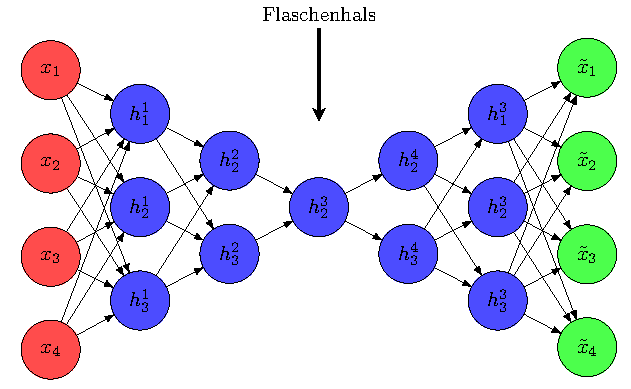
\includegraphics[width=0.6\textwidth]{ae2.pdf}
  \caption{Schichten eines tieferen Autoencoders}
  \label{fig:big_autoencoder}
\end{figure}

\section{Funktionsweise}
Ein Autoencoder möchte die Features $\vec{x}$ von der Inputschicht in die
Outputschicht kopieren. Jedoch zwingt der Flaschenhals den Autoencoder dazu, eine
neue Repräsentation der Features zu erlernen. Dies aus dem Grund, weil die
Features in ihrer jetzigen Form keinen Platz im Flaschenhals finden, da $p \ll d$.
Daher muss das Modell die Informationen der Features
auf nur einige wenige relevante Eigenschaften komprimieren.
Das Modell muss gewissermassen einen Code entwickeln.
Diese neue Repräsentation nennt man das \keyword{Encoding}. \\
In einem zweiten Schritt muss der Autoencoder aus diesem Encoding wiederum
versuchen, die ursprünglichen Features zu rekonstruieren. Diese Rekonstruktion
bezeichnet man als das \keyword{Decoding}.

\paragraph{Encoder und Decoder}
Ein Autoencoder in zwei Teilmodelle untergliedern werden. Das
eine Modell erzeugt das Encoding und das andere das Decoding. Dafür wird
die Hypothesenfunktion $h$ in ein Funktionenpaar $(\phi,\psi)$ aufgespaltet.
\begin{itemize}
\item{$\phi: \fspace{X} \to \fspace{E}$ Encoder-Funktion}
\item{$\psi: \fspace{E} \to \fspace{X}$ Decoder-Funktion}
\end{itemize}
Die erste Teilfunktion $\phi$ ist für das Encoding zuständig. Sie
bildet den Inputraum $\fspace{X} \subseteq \set{R}^d$ auf
den Encodingraum $\fspace{E} \subseteq \set{R}^p$ ab, welcher die neue
Repräsentation $\vec{x^*}$ enthält. Der Inputraum $\fspace{X}$ enthält
sämtliche Features $\vec{x}$.
\para{}
Das Gegenstück ist die Teilfunktion $\psi$. Sie bildet den Encodingraum
$\fspace{E}$ zurück auf den Inputraum $\fspace{X}$ ab.
\para{}
Der Output des Autoencoders $\vec{\hat{x}}$ wird somit durch die aufeinander
folgende Anwendung der Teilfunktionen auf die Features $\vec{x}$ gebildet:
\begin{equation}
  \vec{\hat{x}} = \psi(\phi(\vec{x})) = (\psi \circ \phi)(\vec{x})
\end{equation}

Beim Trainieren wird die Kostenfunktion des Modells minimiert.
Beispielsweise kann dafür die MSE-Kostenfunktion $C_{\text{MSE}}$ dienen.
Wird sie als Kostenfunktion verwendet, so wird folgender Ausdruck minimiert:
\begin{equation}
  \min_{\phi,\psi} {(\vec{x} - \vec{\hat{x}})}^2 = \min_{\phi,\psi} {(\vec{x} - (\psi \circ \phi)(\vec{x}))}^2
\end{equation}
Anders ausgedrückt wird versucht, Funktionen $\phi$ und $\psi$ zu finden, welche
die Differenz zwischen den ursprünglichen Features $\vec{x}$ und den Rekonstruktionen
$\vec{\hat{x}}$ minimieren. Dabei muss der Autoencoder
eine Dimensionalitätsreduktion betreiben. Er entwickelt einen Code, um die Features
in der Flaschenhalsschicht komprimiert zu repräsentieren. Durch die
Kapazitätseinschränkung $p \ll d$ muss $\fspace{E}$ eine niedrig-dimensionale
Codierung der Features darstellen. Dem Modell ist es nicht möglich, die Inputs
identisch wiederherzustellen, da bei der Abbildung $\phi$ Informationen verloren
gegangen sind. Dadurch sollte der Code im optimalen Fall nur noch die Merkmale
der Features umfassen, welche die umfangreichsten Informationen beinhalten.
Nur so kann die bestmögliche Rekonstruktion vollzogen werden, um minimale Kosten
zu erzeugen.
Dieser Code kann extrahiert werden, um eine Repräsentation der Features zu
erhalten, welche nicht mehr mehrere hundert Merkmale umfasst, sondern nur noch einige
wenige. Jegliche natürliche Schwankung in den Werten der Features geht
verloren, die nicht verallgemeinert werden kann. Solche natürlichen Schwankungen
bezeichnet man als \keyword{Datenrauschen}.

\paragraph{Der Code}
Es ist wichtig zu erkennen, dass der Code, welcher der Autoencoder entwickelt,
\keyword{datenspezifisch} ist. Das heisst, er kann nicht wie z.B. ein
Bildkompressionsalgorithmus auf beliebige Daten angewendet werden. Stattdessen
ist er nur sinnvoll für die Kompression von Daten verwendbar, mit welchen er trainiert
wurde.
\para{}
Die Codeentwicklung eines Autoencoders kann man sich ungefähr so vorstellen:
Ein Autoencoder wird mit einem Datensatz von Bildern meschlicher Gesichter trainiert.
Anstatt, dass der Autoencoder die Farbkomponenten der Pixel im Encoding speichert, würde er
die Features abstrahieren. Er würde Information zum Augenabstand, zur
Nasenbreite, zur Augenfarbe usw. als Code verwenden, welche einen deutlich geringeren
Informationsgehalt aufweisen als sämtliche Pixel. Diese Informationen reichen
aber aus, um realtiv gute Rekonstruktionen zu erzeugen.

\section{Anwendungen}
Die Eigenschaft, welche einen Autoencoder für die diverse
Anwendungen geeignet macht, ist die Dimensionalitätsreduktion.
Wir werden nun eine Anwendung grob betrachten und eine weitere detailliert
in der nächsten Sektion: der Denoiser.

\subsection{Datenkompression}
Durch die Dimensionalitätsreduktion besitzt das Encoding einen geringeren
Informationsgehalt als die ursprünglichen Daten. Aus diesem Grund kann der
Autoencoder zur Datenkompression verwendet werden. Die komprimierten Daten
können somit platzsparender gespeichert oder über das Internet versendet werden.
Die komprimierten Daten benötigen um den Faktor $\frac{p}{d}$ weniger Speicher,
wobei $p$ die Grösse des Flaschenhalses und $d$ die Grösse
der Inputschicht ist.
Mithilfe des Decoders können die ursprünglichen Daten zurückgewonnen werden.
Jedoch hat das Decoding einen gewissen Qualitätsverlust im Vergleich zu den
Features erlitten. Somit können die Daten nicht in voller Qualität rekonstruiert
werden. Es handelt sich also um eine \keyword{verlustbehaftete Kompression}.
Ausserdem ist diese Kompression datenspezifisch. Das heisst, dass ein
Autoencoder, welcher darauf trainiert wurde, Bilder von Katzen zu komprimieren,
nur sehr schlechte Rekonstruktionen für Landschaftsbilder erzeugen würde. Dies
steht im Gegensatz zu einer JPEG-Kompression, welche sich für beliebige
Bilder eignet, aber geringere Kompressionsraten aufweist als Autoencoder.
\para{}
Eine andere datenspezifische Kompressionsmethode stellt die
\keyword{Hauptkomponentenanalyse} (PCA) dar. Sie ist eine erweiterte Version der
Hauptachsentransformation, welche benötigt wird, um Kegelschnitte in
Standardlage zu bringen. Falls ausschliesslich lineare Neuronen in einem
Autoencoder verwendet werden, ist das Verhalten des Modells sehr ähnlich zu PCA.
Jedoch sind Autoencoder grundsätzlich PCAs überlegen, da sie mithilfe von
nicht-linearen Neuronen komplexere Kompressionsmethoden entwickeln können.

\para{}
Quellen: \cite{paper:autoencoder_compression} \cite{paper:pca}


\section{Convolutional-Autoencoder}\label{sec:convolutional_autoencoder}
Ein Convolutional-Autoencoder ist, wie es der Name schon andeutet, ein Autoencoder,
welcher anstatt der normalen Fully-Connected-Schichten eines KNNs, die Schichten eines CNN verwendet.
Dieser ist interessant, weil er zur Dimensionalitätsreduktion von Bildern
verwendet werden kann. Er kann beispielsweise als Bildkompressionsalgorithmus
genutzt werden.
\para{}
Wie bei den normalen Autoencodern auch, müssen hier die Inputschicht und das
Decoding die gleiche Form aufweisen. Nun ist auch ersichtlich, weshalb es in
Sektion \refbox{sec:dimensionalitätskontrolle} wichtig war, CNN-Schichten zu
entwickeln, welche ein willentliches Einstellen der Schichtgrössen erlauben.
Es muss versucht werden, dass die Vergrösserung nach dem Flaschenhals die
Verkleinerung vor dem Flaschenhals kompensiert.
Eine Massnahme dafür ist, bei sämtlichen Convolutional-Schichten Same-Padding zu
verwenden und die Dimensionalität nur über Pooling- und UpSampling-Schichten zu
steuern. Des Weiteren muss der Decoder den spiegelverkehrten Aufbau zum Encoder
aufweisen, wobei Pooling-Schichten durch UpSampling-Schichten ersetzt werden.
\para{}
In Abbildung \refbox{fig:convolutional_autoencoder} ist ein schematischer
Convolutional Autoencoder aufgezeigt. Dieser verarbeitet ein farbiges Bild mit
drei Farbkomponenten.
\para{}
\begin{figure}[h!]
  \centering
  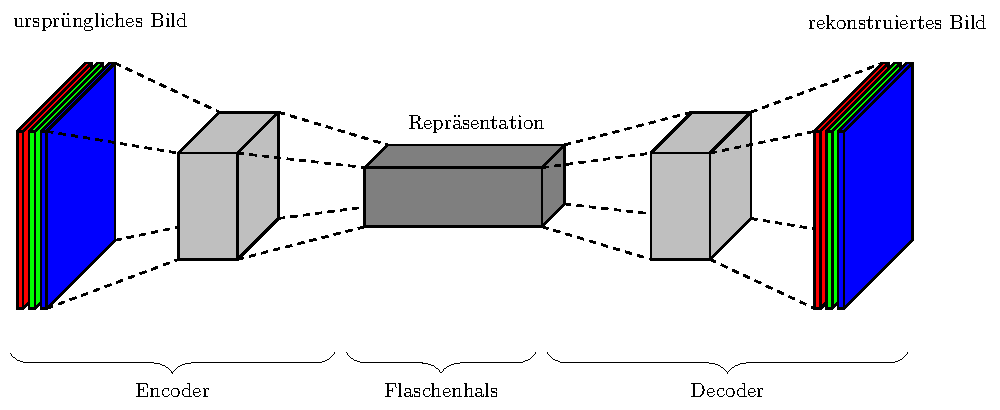
\includegraphics[width=0.9\textwidth]{cae.pdf}
  \caption{Darstellung eines Convolutional Autoencoders}
  \label{fig:convolutional_autoencoder}
\end{figure}
\para{}
Ausserdem sind Convolutional-Autoencoder von Interesse, da sie zu einer weiteren
Anwendung führen: zum Denoising-Autoencoder.
Dieser wird im nächsten Abschnitt betrachtet.
\para{}
Quellen: \cite{yt:autoencoder_faces}

\section{Denoising-Autoencoder}
Ein Denoising-Autoencoder oder einfach Denoiser verkörpert einen leicht abgeänderten
Autoencoder. Er wird vor allem verwendet, um das Bildrauschen aus Bildern zu entfernen.
\para{}
Im Unterschied zu klassischen Autoencodern benötigt er einen Datensatz mit
wahren Labels, da er nicht die Features kopiert.
Seine Inputs bestehen aus den verrauschten Bildern. Die Labels sind die
unverrauschten Bilder. Somit wird er darauf trainiert, das Rauschen zu entfernen.
Man mag sich nun die Frage stellen, weshalb hierfür ein Autoencoder und
kein normales CNN verwendet wird. Empirisch hat sich gezeigt, dass
Denoiser besser für das Entrauschen von Bildern geeignet sind.
Das hat nachvollziehbare Gründe. Bei der
Entwicklung des Codes für Encoding-Repräsentation, kann das Rauschen nicht
codiert werden, da es völlig zufällig auftritt. Es existieren keine Muster oder
Gesetzmässigkeiten, welche anders codiert werden könnten. Somit muss der
Autoencoder diese Rausch-Features verwerfen. Gegenüber sonstigen CNNs hat er ein leichteres Spiel.
\para{}
In Abbildung \refbox{fig:denoiser} ist ein Denoiser abgebildet, welcher ein
graustufiges Bild mit nur einer Farbkomponente entrauscht.
\para{}
\begin{figure}[h!]
  \centering
  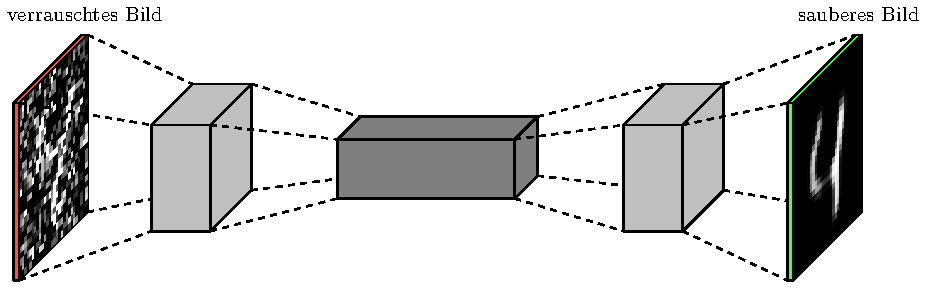
\includegraphics[width=0.8\textwidth]{cdae.pdf}
  \caption{Visualisierung eines Convolutional-Denoising-Autoencoder}
  \label{fig:denoiser}
\end{figure}
\para{}
Quellen: \cite{paper:denoiser}

\subsection{Generierung der verrauschten Bilder}
Ein Denoising-Autoencoder kann verwendet werden, um diverse Arten von
Rauschen zu entfernen. Jedoch werden wir uns in dieser Arbeit auf ein
generiertes Rauschen beschränken: das additive Gauss'sche Rauschen.
Um es zu erzeugen, wird eine Gauss'sche Normalverteilung
$\mathcal{N}(\mu = 0, \sigma^2 = 1)$ verwendet mit Erwartungswert $\mu = 0$ und Varianz
$\sigma^2 = 1$. Für jedes Feature des Datensatzes wird dieser Verteilung ein
Zufallswert entnommen. Dieser Wert wird mit einem Rauschfaktor $c$
multipliziert, welcher die Rauschstärke bestimmt. Das Resultat wird zum
entsprechenden Wert des Features addiert.
Auf diese Weise lässt sich ein verrauschter Datensatz entwickeln.
\begin{gather*}
  r \sim \mathcal{N}(\mu = 0, \sigma^2 = 1) \\
  \tilde{x} = x + c \cdot r
\end{gather*}

\begin{figure}[h!]
  \centering
  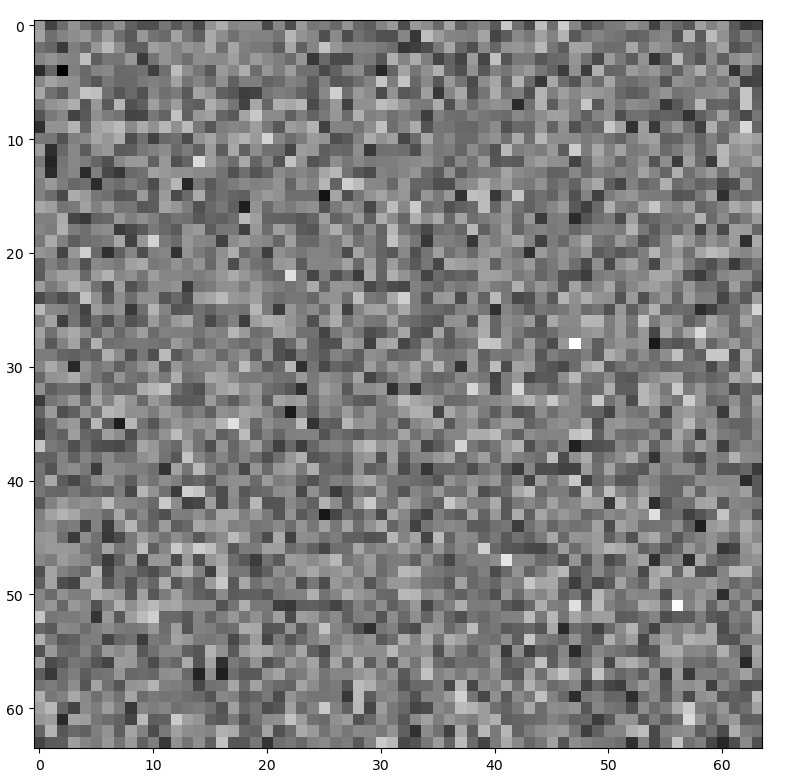
\includegraphics[width=0.3\textwidth]{gauss_noise.png}
  \caption{zwei-dimensionales Gauss'sches Rauschen mit Rauschfaktor $c=1$}
\end{figure}
\para{}
Quelle: \cite{wiki:gauss_noise}

% ------------------------------------

\chapter{Frameworks für Maschinelles Lernen}
In den Kapiteln eins bis vier wurde die theoretische Funktionsweise von
Maschinellem Lernen anhand von zwei konkreten Architekturen (CNN und
Autoencoder) eines KNNs dargelegt.
Nun findet ein Übergang zur praktischen Programmierung eines
Convolutional-Denoising-Autoencoders statt. Es wird hier die grobe Funktionsweise der
Frameworks TensorFlow und Keras erörtert. Aus didaktischen Gründen wird die
Verwendung isoliert betrachtet.
Sie dient als Vorbereitung auf das Kapitel sechs, wo der Gesamtzusammenhang anhand der
fallbezogenen Programmierung hergestellt wird.
\para{}
\bigskip

\section{TensorFlow}\label{sec:tensorflow}
\keyword{TensorFlow} (TF) ist ein von Google entwickeltes \keyword{Framework} für
\keyword{datenstromorientierte Programmierung}. Es ist im Grunde genommen eine
Mathematik-Programmbibliothek für numerische Berechnungen, dessen Hauptanwendungsbereich im Maschinellen Lernen
liegt. TF zeichnet sich hauptsächlich durch seine einfache Bedienung aus, welche
es dem Benutzer erlaubt, ohne grosse mathematische Vorkenntnisse, ein ML-Modell
zu entwickeln. Des Weiteren sind die performanten
Implementierungen bemerkenswert, welche den Trainingsvorgang sehr kurz halten.
Daher ist TF gegenüber selbst geschriebenen Implementierungen zu bevorzugen.
TF ist gratis und ein Open-Source-Projekt. Es steht auf Github zur Verfügung
(siehe QR-Code).
\begin{wrapfigure}{L}{2cm}
  \qrcode[height=2cm]{https://github.com/tensorflow/tensorflow}
  \captionof{figure}{QR-Code zum GitHub-Repo}
\end{wrapfigure}
In der Industrie ist TensorFlow gut etabliert und weit verbreitet. Es wird von
vielen grossen Internetunternehmen verwendet. Einige dieser
Firmen sind: Google, Twitter, AirBnB, Intel, Snapchat und noch viele mehr.
\para{}
Grundsätzlich wurde TF für Maschinelles Lernen entwickelt. Speziell eignet es
sich für Deep Learning. Es bietet die nötigen Werkzeuge, um ein Modell zu
definieren und es mit den eingebauten Algorithmen zu trainieren.
Trotz des engen Bezugs zum Maschinellen Lernen, eignet sich TF darüber hinaus auch für
andersartige Anwendungen, welche Gebrauch von numerischen Berechnungen machen.
\para{}
Im Folgenden wird die grobe Funktionsweise von TensorFlow untersucht. Wir
beziehen uns dabei auf TensorFlow-Core Version r1.14%
\footnote{Momentan befindet sich TF 2.0 in der Beta Version. Es handelt sich
  dabei um eine grosse Überarbeitung des Frameworks. Sobald TF 2.0 offiziell
  veröffentlich wurde, ist es zu empfehlen, diese zu verwenden.}.
Die Betrachtung von TF wird hier bewusst kurz gehalten, da bei der
Programmierung in Kapitel sechs auf die High-Level-API Keras zurückgegriffen
wird. Mit TF wird daher nur teilweise direkt gearbeitet. Trotzdem ist es hilfreich, ein
grobes Verständnis über TF zu besitzen, um die Funktionsweise zu verstehen.
\para{}
Die wichtigste Quelle, um TensorFlow zu erlernen, ist die offizielle TensorFlow
Website. Dort findet man auch die Dokumentation.
\begin{wrapfigure}{L}{2cm}
  \qrcode[height=2cm]{https://www.tensorflow.org/api/stable}
  \captionof{figure}{QR-Code zu den Docs}
\end{wrapfigure}
\para{}
Quellen: \cite{book:tensorflow} \cite{net:tf_docs}

\subsection{Frontend und Backend}
Wie die meisten grossen Frameworks ist TensorFlow in Backend und
Fontend aufgeteilt.
\para{}
\begin{infobox}{Fontend und Backend}
  Das \keyword{Frontend} ist der Teil eines Programms, mit welchem der Benutzer
  interagiert. Es stellt eine Schnittstelle zum sogenannten Backend eines
  Programms dar. Es offenbart so gewisse Funktionalitäten des Programms,
  ohne die zugrunde liegenden Logik preiszugeben.
  \para{}
  Das \keyword{Backend} ist das Gegenstück zum Frontend. Es implementiert
  jegliche Programmlogik, welche das gewünschte Verhalten der Applikation
  hervorruft. Der Benutzer hat keinen direkten Zugriff auf diesen Teil des
  Programms und bekommt somit nichts direkt von dessen Existenz mit.
\end{infobox}
\para{}
Das Frontend von TF ist in \keyword{Python} geschrieben%
\footnote{
  TF besitzt mehrere Frontends, welche in den verschiedensten
  Programmiersprachen geschrieben sind. Wir werden jedoch nur das
  Python-Frontend betrachten, da es am besten von TF unterstützt ist.
}.
Python wird allgemein als eine sehr einsteigerfreundliche Programmiersprache wahrgenommen. Sie
ermöglicht es dem Benutzer, mit vergleichsweise wenig Programmcode TensorFlow intuitiv zu verwenden.
In Kapitel sechs wird die Entwicklung eines Modells in Python vorgenommen.
\para{}
Das Backend von TF ist dagegen in \keyword{C++} (und CUDA)
geschrieben. C++ ist im Gegensatz zu Python sehr performant.
Daher ist die Ausführungszeit eines Programms sehr kurz. In
der Konsequenz ist der Programmcode deutlich anspruchsvoller und
ausführlicher (engl.: verbose) geschrieben.
Da der Benutzer jedoch keine direkte Interaktion mit dem Backend hat, muss er
auch nicht mit C++ vertraut sein.
\para{}
Die hohe Performance von TF wird durch verschiedene Designentscheidungen garantiert.
Falls der Leser am besseren Verständnis dieser Entscheide und der eigentlichen
Implementierung des Backends interessiert ist, findet er im Anhang
\refbox{sec:anhang_tf} weitere Informationen dazu vor.

\subsection{Graph}
TensorFlow ist datenstromorientiert, was bedeutet, dass eine Berechnung
durch einen gerichteten Graphen beschrieben wird. Zuerst wird ein solcher Graph
aufgestellt und es werden Knoten und Pfade hinzugefügt. Erst nach dieser
Definition wird er ausgeführt.
Es handelt sich dabei um einen \keyword{Computational Graph}, welcher schon in
Anhang \refbox{sec:anhang_bp} erwähnt wurde.
In TensorFlow wird er vereinfacht als \keycode{Graph} bezeichnet.
\para{}
Dieser Graph führt eine Datenstrom-Berechnung aus.
Er besteht aus einer Menge an Knoten, welche miteinander über Pfade
verbunden sind. Die Knoten und die Pfade bilden die Operationen, welche auf die
Zahlenwerte angewandt werden. Die Resultate landen jeweils im neuen Knoten.
Jeder Knoten hat null oder mehr Inputs und null oder mehr Outputs.
Zur Definition des Graphs müssen lediglich die Operationen festgelegt werden.
\para{}
Mithilfe des Graphs wird das eigentliche ML-Modell definiert. Die Ausführung von
ihm stellt die Vorwärtspropagierung dar.
\para{}


\subsubsection{Knoten als Tensoren}
Die zentrale Dateneinheit in TF sind Tensoren, welche bereits in Sektion
\refbox{sec:tensor} dargelegt wurden. Auch die Knoten des Graphen
verkörpern Tensoren. Die meisten jedoch enthalten keine festen Zahlenwerte,
sondern werden erst bei der Ausführung des Graphen mit Werten gespeist. Danach können
die Werte ausgelesen werden.
\para{}
Die Tensoren erlauben es den Daten, innerhalb des Graphen beliebige
Dimensionen und Formen anzunehmen. Es können
sowohl Listen von Zahlen (Vektoren), wie auch Bilder (Tensoren dritter Stufe)
verrechnet werden. Aus diesem Grund war es auch sinnvoll, in Sektion
\refbox{sec:forward} und im Anhang \refbox{sec:anhang_bp} die Gleichungen in
Matrixform herzuleiten.
\para{}
Ein \keycode{Tensor} ist definiert durch seine Form und den Datentyp seiner
Elemente. Fast alle Tensoren sind mit einer einzigen Graph-Ausführung
assoziiert. Sie besitzen ihren Wert nur für den jeweiligen Durchlauf, danach wird
er verworfen. Man sagt die Tensoren sind ``immutable'', da die Werte nicht
erhalten bleiben und daher auch nicht modifiziert werden können.
\para{}
Die meisten Knoten innerhalb des Graphen verkörpern Operationen, jedoch gibt es
noch einene anderen speziellen Typ von Knoten: Inputknoten.
Diese wirken als Startpunkt des Graphen, bei welchem die
Ursprungswerte eingespiesen werden.
Sogenannte \keycode{placeholder} dienen beispielsweise dazu, die Features ins Modell einzufügen.
Hingegen können \keycode{variable}-Inputknoten genutzt werden, um Modellparameter einzuführen.
Diese Modellparameter-Tensoren sind im Gegensatz zu den vorgängig beschriebenen Tensoren
``mutable''. Ihre Werte bleiben über mehrere Graphenausführungen hinweg erhalten und
können auch beim Training modifiziert werden.


\subsubsection{Operationen}
Die Werte der Inputknoten gelangen über die Pfade zu den nächsten Knoten. Dort
werden diese durch verschiedene \keyword{Operationen} weiterverrechnet.
Durch das Definieren einer Operation wird automatisch ein neuer Knoten
erstellt, in welchem das Resultat landet. Auch die benötigen Pfade werden
von selbst vernetzt.
Eine Operation besitzt jeweils einen Namen und repräsentiert eine
abstrakte Berechnung. Sie besitzt jeweils null oder mehr Tensor-Objekte als
Input, wie auch als Output.
\para{}
TensorFlow offeriert eine Vielzahl von vordefinierten Operationen, sodass eine eigenständige
Definition von Operationen meistens nicht notwendig ist.
Ein Beispiel für eine vordefinierte Operation ist die
\keycode{matmul(a,b)}-Operation. Sie stellt eine Matrixmultiplikation zwischen
dem Knoten \mintinline{python}{a} und dem Knoten \mintinline{python}{b} dar.
Das Resultat kann dann in einer neuen Knotenvariable \mintinline{python}{c} gespeichert werden.
\para{}
Um den eigentlichen Graph zu erstellen, werden zu Beginn einige Inputknoten
definiert. Diese werden durch die vordefinierten Operationen abgebildet.
Die jeweiligen Resultate können weiter verrechnet werden bis dann der gewünschte Graph
entsteht.
\para{}
\bigskip
In Abbildung \refbox{fig:graph} ist ein Beispielsgraph visualisiert. Dieser
weist dasselbe Verhalten auf wie ein künstliches Neuron mit drei Inputs. In rot sind
sind die \code{Placeholder}-Tensoren und in blau die \code{Variable}-Tensoren dargestellt.

\begin{figure}[h!]
  \centering
  \begin{tikzpicture}[nodes={draw,circle,inner sep=0, minimum size=1cm},>=latex]
    \tikzstyle{inp} = [fill=red!70!pagecolor]
    \tikzstyle{param} = [fill=blue!70!pagecolor]


    \tikzstyle{arr} = [thick,<-]


    \node[inp] (x1) at (0,2) {$x_1$};
    \node[param] (w1) at (1.5,3) {$w_1$};
    \node[] (+1) at (3,2) {$\times$};
    \draw[arr] (+1) edge (x1) edge (w1);

    \node[inp] (x2) at (0,0) {$x_2$};
    \node[param] (w2) at (1.5,1) {$w_2$};
    \node[] (+2) at (3,0) {$\times$};
    \draw[arr] (+2) edge (x2) edge (w2);

    \node[inp] (x3) at (0,-2) {$x_3$};
    \node[param] (w3) at (1.5,-1) {$w_3$};
    \node[] (+3) at (3,-2) {$\times$};
    \draw[arr] (+3) edge (x3) edge (w3);

    \node[param] (b) at (5,3) {$b$};

    \node[] (sum) at (5,0) {$\Sigma$};
    \draw[arr] (sum) edge (+1) edge (+2) edge (+3) edge (b);

    \node[] (act) at (7,0) {$\varphi$};
    \draw[arr] (act) edge (sum);

  \end{tikzpicture}
  \caption{Beispielsgraph, welcher sich wie ein künstliches Neuron verhält}
  \label{fig:graph}
\end{figure}

\subsection{Ausführung}
\subsubsection{Session}
Als Schnittstelle zwischen Frontend und Backend fungiert die sogenannte
\keycode{Session}. Sie leitet die Informationen zum Graphen an das Backend weiter, damit er
dort performant ausgeführt werden kann.
Die Kernaufgabe einer Session besteht darin, den Graphen mehrfach auszuführen.
Diese Ausführungen repräsentieren die Vorwärtspropagierung.
Dabei kann der Benutzer die Knoten angeben, deren Werte er nach der
Ausführung ausgewiesen haben möchte. Die Ausführungsfunktion erwartet als Argumente
diejenigen Werte, mit denen die Inputknoten gespeist werden sollen.


\subsubsection{Optimizer}
Bevor das definierte Modell brauchbare Resultate bei der Graphenausführung
liefern kann,
muss es trainiert werden. Dafür kommt ein sogenannter \keycode{Optimizer} zum Einsatz.
Dieser verkörpert das gewählte Optimierungsverfahren, welches zur Minimierung
der Kostenfunktion verwendet wird.
Es gibt verschiedene Optimizer, welche unterschiedliche
Konvergenzgeschwindigkeiten und Präzisionsgrade aufweisen.
Im Rahmen dieser Arbeit wurde jedoch nur das SGD-Verfahren behandelt, sodass
ausschliesslich dieser Optimizer hier Anwendung findet.
\para{}
Beim Optimierungsverfahren muss TF die partiellen Ableitungen der Kostenfunktion
bezüglich den Modellparametern bestimmen. Hierfür macht sich die Verwendung von
Computational Graphs ausgezahlt, da mithilfe von ihnen der Kostengradient
automatisiert bestimmt werden kann (siehe Anhang \refbox{sec:anhang_bp}).

\subsection{Tensorboard}
TensorBoard ist ein externes Zusatzprogramm zu TensorFlow. Mit dessen Hilfe können
Daten zum Modell-Graph und zum Trainingsprozess erfasst und visualisiert werden.
Wertvoll ist vor allem, dass die Kostenfunktionsentwicklung betrachtet werden
kann.
\para{}
TensorBoard ist als Webserver geschrieben und kann über einen Webbrowser
benutzt werden.
TensorBoard ist als Callback in TensorFlow zu aktivieren, damit die
nötigen Daten während der Graphausführung gesammelt werden.

\begin{figure}[h!]
  \centering
  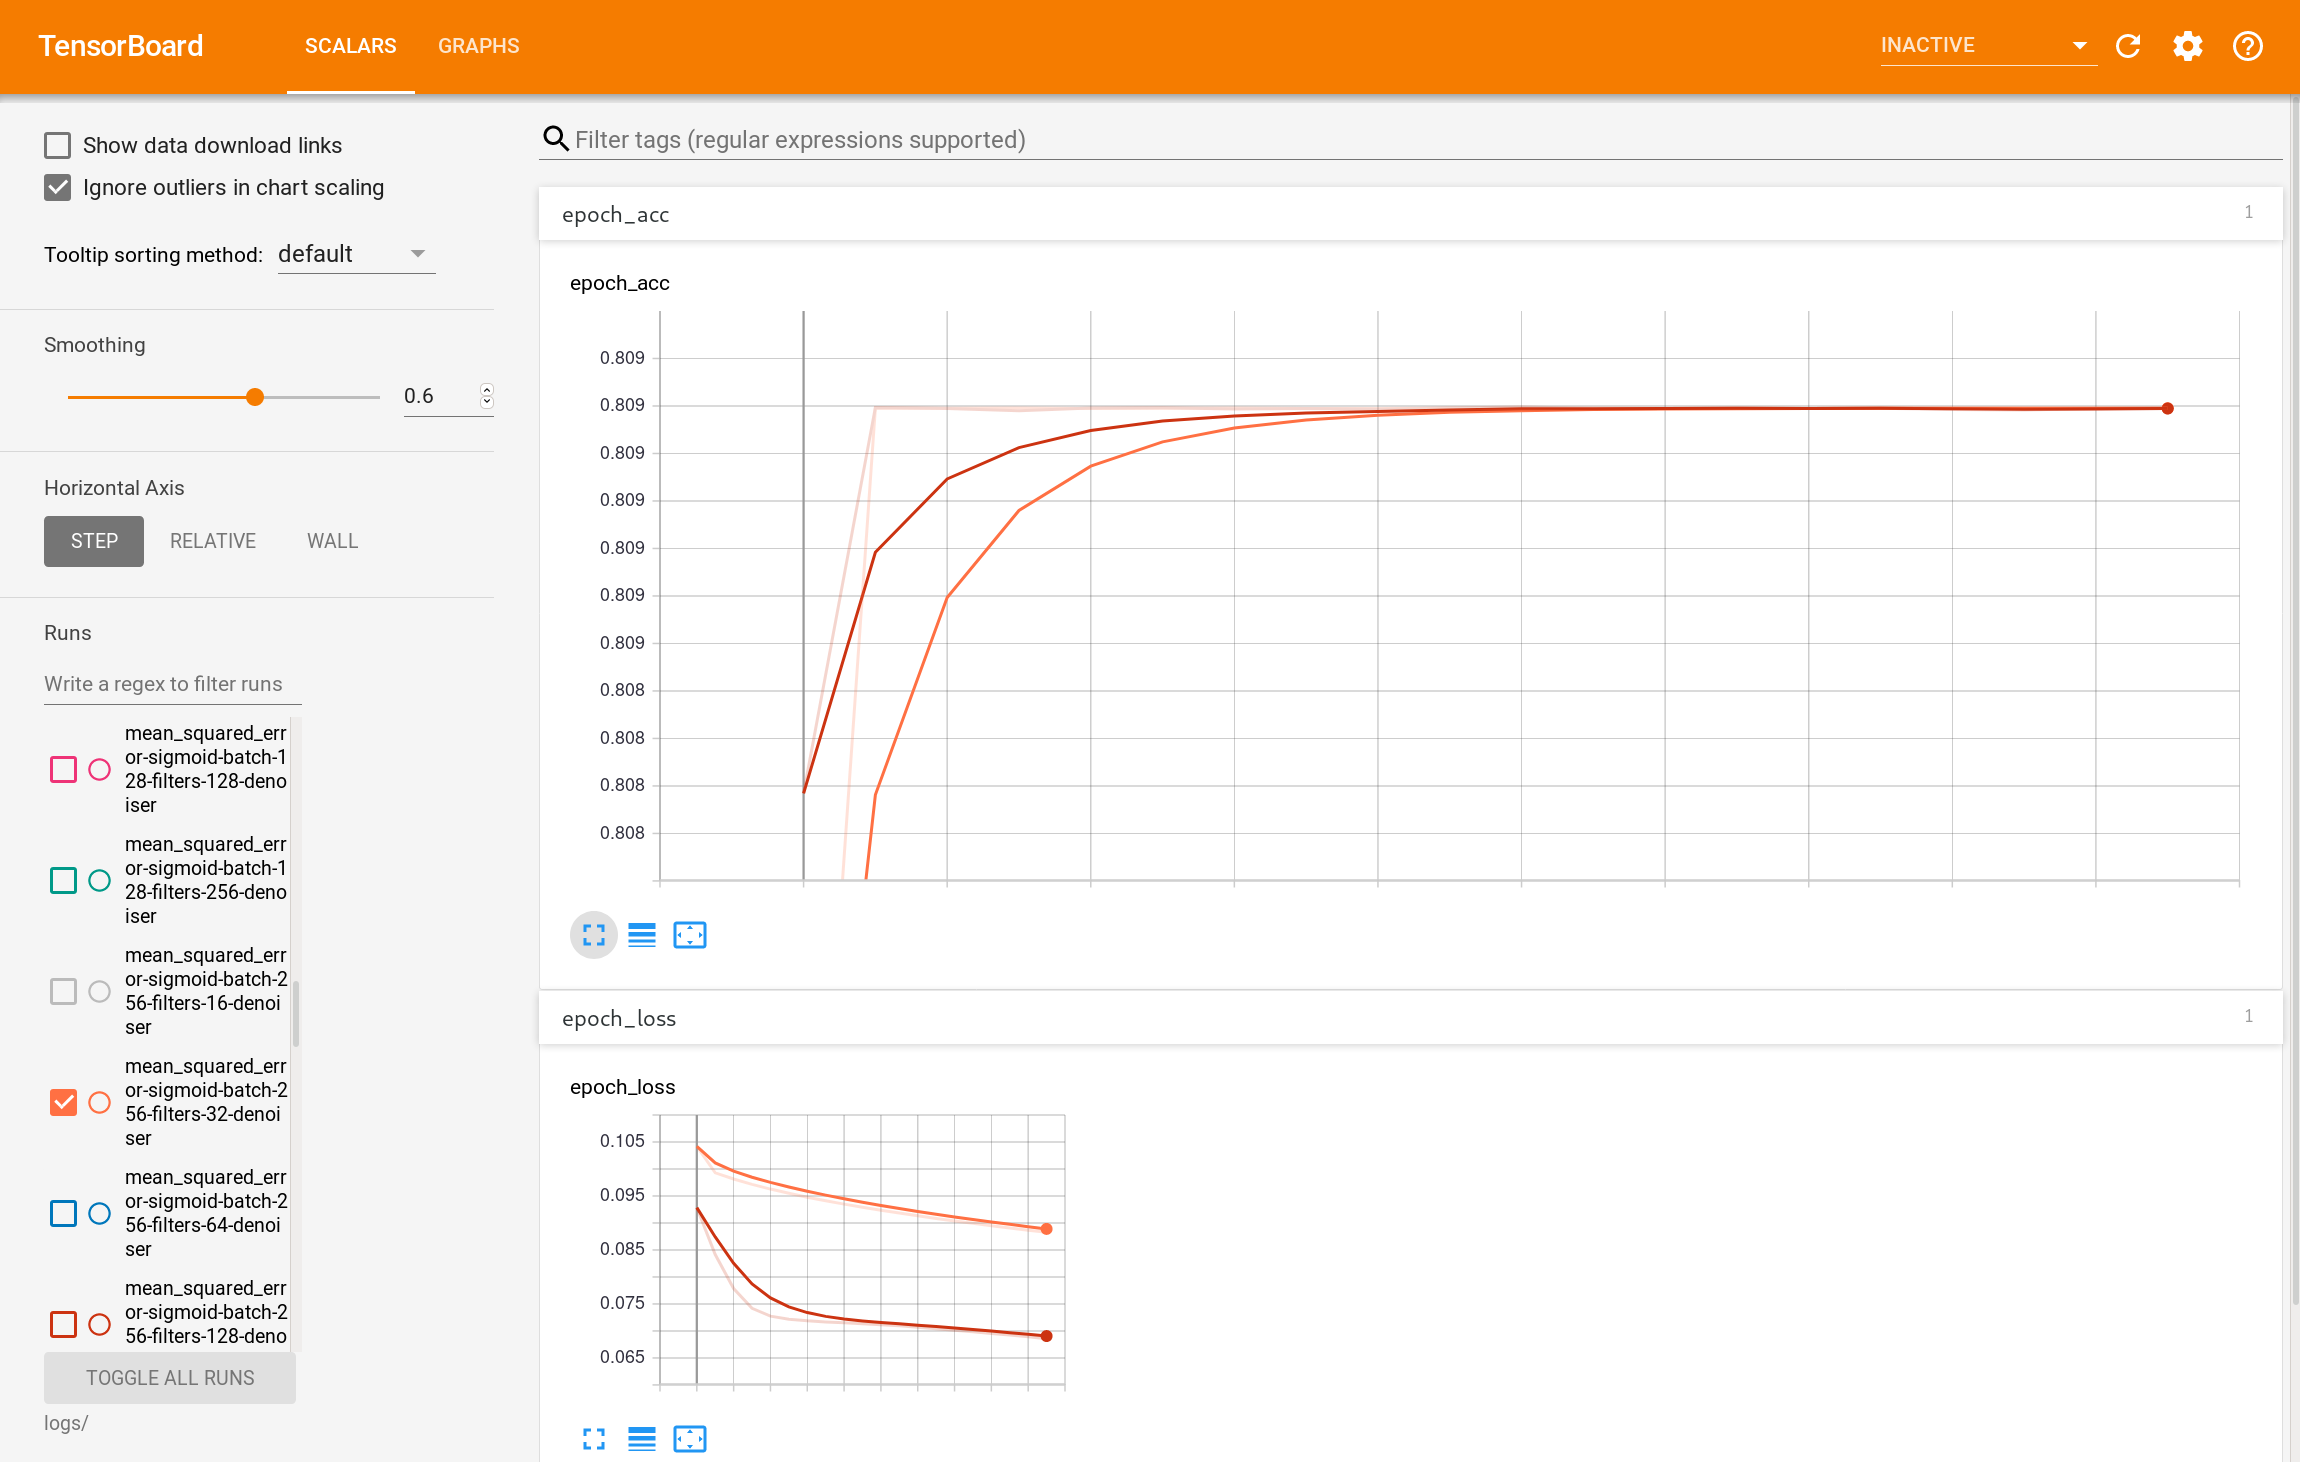
\includegraphics[width=0.7\textwidth]{tensorboard.png}
  \caption{das TensorBoard-Webinterface}
\end{figure}

\subsubsection{Hyperparameter einstellen}
Der wichtigste Aspekt von TensorBoard ist, dass die Trainingsfortschritte
visualisiert werden.
Dadurch können die verschieden Funktionsgraphen der Kostenfunktion analysiert werden.
Es ist sogar möglich, die Kostengraphen mehrerer Modelle gleichzeitig anzuzeigen und zu vergleichen.
Somit kann man verschiedene Modelle mit unterschiedlichen Hyperparametern
gegenüberstellen und somit die besten Hyperparameter identifizieren.
Dieses Verfahren gelangt in Kapitel sechs zur Anwendung.
Ebenfalls wird die beanspruchte Trainingszeit angezeigt und so beurteilbar gemacht.
\para{}
In der unten stehenden Abbildung ist ein Graph von TensorBoard dargestellt,
welcher die Entwicklung der Kostenfunktion für den Testdatensatz verschiedener
Modelle anzeigt. In diesem Beispiel hätte die unterste orange Kurve am besten
abgeschnitten. Dieses Modell hat die kleinsten Kosten verursacht. Jedoch hat
dieses auch die längste Trainingszeit beansprucht.

\begin{figure}[h!]
  \centering
  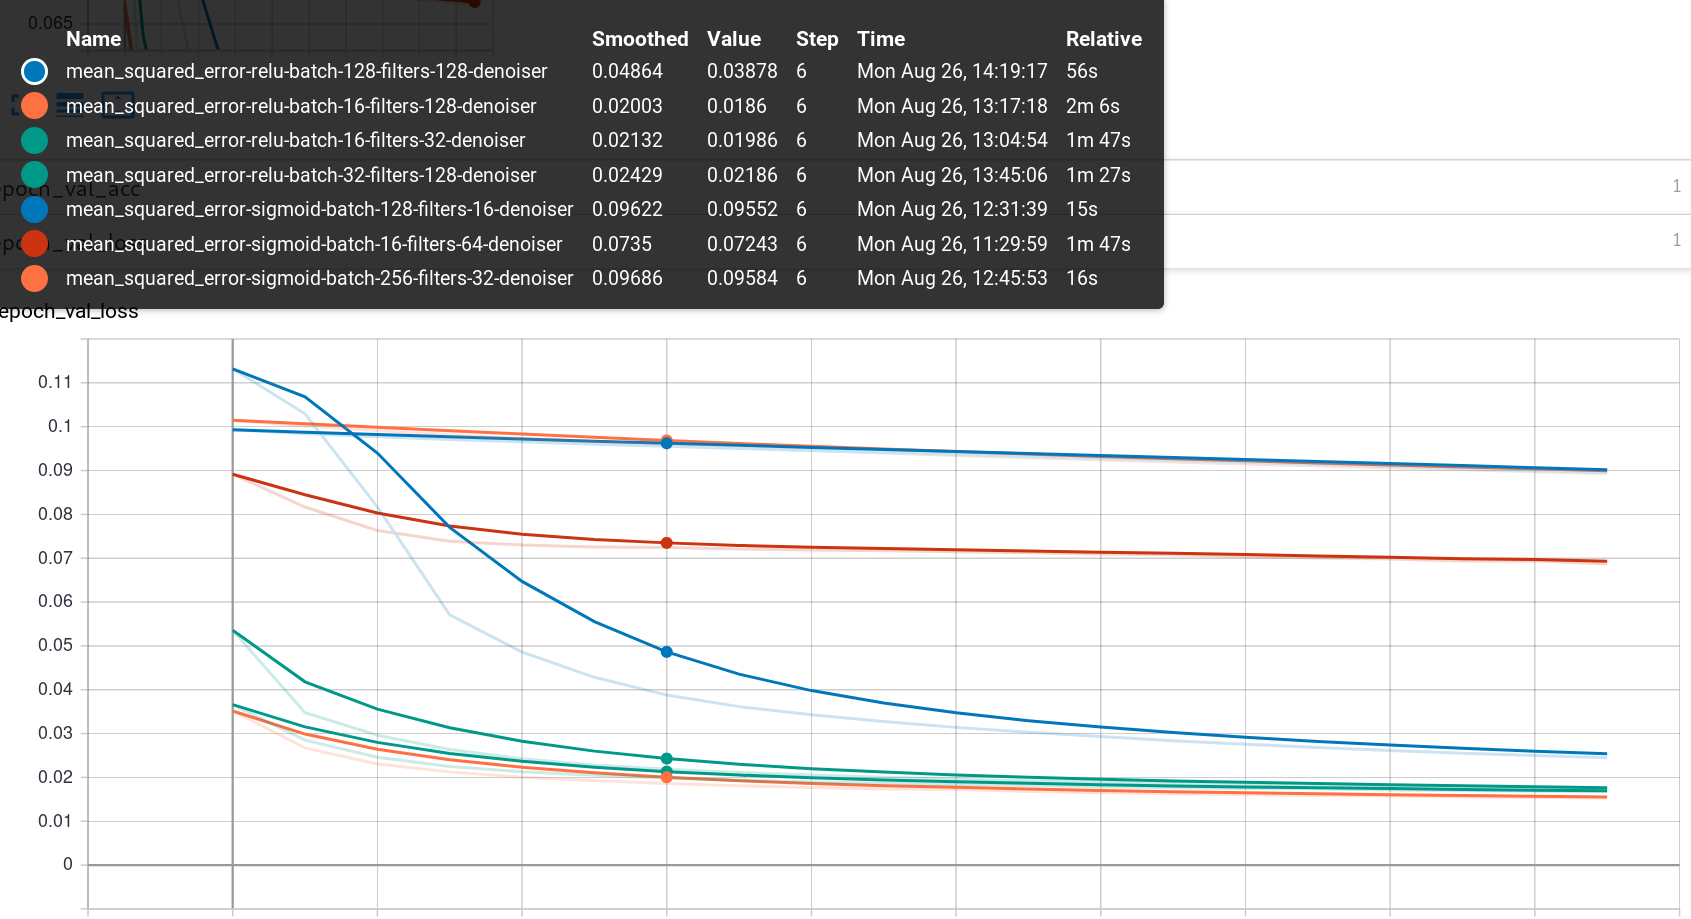
\includegraphics[width=0.7\textwidth]{tensorboard_graph.png}
  \caption{Trainingsvisualisierungen in TensorBoard}
\end{figure}
\para{}

\section{Keras}
Die Erstellung von KNNs in TensorFlow erweist sich als vergleichsweise aufwendig, weil jede
KNN-Schicht manuell zu konstruieren ist.  Aus diesem Grund soll nun die
Funktionsweise von Keras behandelt werden. \keyword{Keras} ist eine High-Level
API, welche verschiedene KNN-Schichten vorkonfiguriert zur Verfügung stellt. Somit müssen diese
nicht mehr manuell erstellt werden, was allfällige Fehler vermeidet.
\para{}
Keras ist ein Deep-Learning Framework, geschrieben in
Python. Es wurde entwickelt, um eine einheitliche Schnittstelle für
verschieden Backends, wie TensorFlow, Microsoft Cognitive Toolkit und Theano zu
bieten. Seit der TF Version 1.4 ist Keras ein fester Bestandteil der TensorFlow-Core-API.
Keras ermöglicht ein benutzerfreundliches Definieren von
KNNs, welche dann vereinfacht trainiert werden können.
\para{}
Quellen: \cite{net:keras_docs} \cite{net:tf_docs}

\subsection{Sequential-Modell}
Keras ist keine eigenständige Programmbibliothek, sondern baut auf
TensorFlow auf und dient als High-level Schnittstelle.
Es verwendet die verschiedenen Konzepte von TF, wie Graphen und Operationen,
um eigene KNN-Bestandteile zu implementieren.
Dadurch ist es für den Benutzer deutlich einfacher, ein Modell aus diesem Baukasten
zu konstruieren.
\para{}
Die gängigste Vorgehensweise besteht darin, ein sogenanntes
\keyword{Sequential-Modell} zu bauen.
Dies ist ein Modell, welches einen linearen Stapel von verschiedenen
KNN-Schichten beinhaltet. Man kann dabei aus den vordefinierten Schichten
wählen. Im folgenden werden diese Schichten näher betrachtet.

\subsection{Schichten}
Die Definition des Graphen in Keras erfolgt, indem die verschiedenen Schichten
des gewünschten Modells in Variabeln gespeichert werden.
Um die Schichten miteinander zu verbinden, erfolgt eine Referenzierung auf die
vorherige Schicht.
Sobald alle Schichten deklariert wurden, wird eine Modellvariable definiert,
welche die erste und die letzte Schicht als Argumente erwartet.
\para{}
Im folgenden werden die relevanten Schichtentypen von Keras dargelegt.
\para{}
Vorgängig sei darauf hingewiesen, dass Keras standardmässig ein anderes Vorgehen
zur Initialisierung der Modellparameter verwendet, als in der Theorie (siehe
Sektion \refbox{sec:parameter_initialisieren}) erklärt wurde.
Keras benutzt nämlich eine Glorot-Initialisierung mit einer uniformen Verteilung.
Dies steht im Gegensatz zur erklärten Theorie, wo eine Normalverteilung verwendet wurde.
Aus diesem Grund muss bei jeder Schicht explizit spezifiziert werden, dass eine
Glorot-Initialisierung mit Normalverteilung angewendet werden soll.

\paragraph{Input-Schicht}
Die Input-Schicht enthält als Platzhalter-Schicht alle Features. Sie besitzt keine
weitere Funktionalität. Mit folgendem Code kann sie definiert werden, dabei muss
lediglich die Form des Featuretensors angegeben werden:
\begin{minted}[frame=lines,framesep=2mm,baselinestretch=1.2,bgcolor=lightgray,fontsize=\footnotesize]{python}
  tf.keras.Input(shape=(<Form>)
\end{minted}

\paragraph{Dense-Schicht}
Die erste richtige KNN-Schicht ist die Fully-Connected-Schicht. Sie wird in
Keras als \keycode{Dense} bezeichnet. Sie ist wie in
der Theorie erklärt, diejenige Schicht, welche aus Neuronen besteht und ``dicht'' zu jedem
Neuron der nächsten Schicht verbunden ist.
Als Argumente erwartet die Schicht die Anzahl Neuronen, aus welcher sie besteht,
die Aktivierungsfunktion und die vorherige Schicht. Wie vorhin erwähnt
überschreiben wir den Standard-Initialisierer mit dem
\code{'glorot\_normal'}-Initialisierer. Ebenfalls wird die vorherige Schicht
referenziert, um die Verbindung zwischen den Schichten herzustellen.
\begin{minted}[frame=lines,framesep=2mm,baselinestretch=1.2,bgcolor=lightgray,fontsize=\footnotesize]{python}
  tf.keras.layers.Dense(<Anzahl Neuronen>,
    activation=<Aktivierungsfunktion>, kernel_initalizer='glorot_normal')(<vorherige Schicht>)
\end{minted}


\paragraph{Conv2D-Schicht}
Die Convolutional-Schicht eines CNNs wird in Keras mit \keycode{Conv2D}
bezeichnet. Sie verhält sich, wie in der Theorie erklärt. Zu ihrer Definition
gehört die Anzahl Filter $c$, die Filtergrösse $f$, der Stride $s$, das Padding
$p$ und die Aktivierungsfunktion $\varphi$.
Die Tensoren, welche von einer CNN-Schicht verarbeitet werden sollen, müssen
folgendes Format ausweisen: $(\text{Anzahl Samples}, \text{Anzahl
  Farbkomponenten}, \text{Bildhöhe}, \text{Bildbreite})$.
\begin{minted}[frame=lines,framesep=2mm,baselinestretch=1.2,bgcolor=lightgray,fontsize=\footnotesize]{python}
  tf.keras.layers.Conv2D(filters=<Anzahl Filter>, kernel_size=<Filtergrösse>,
    strides=<>, padding=<>, activation=<>, kernel_initalizer='glorot_normal')(<vorherige Schicht>)
\end{minted}

\paragraph{MaxPool2D-Schicht}
Die \code{MaxPool2D}-Schicht in Keras ist diejenige Schicht, welche das MaxPooling vornimmt. Um sie zu
definieren, muss die Grösse des Feldes $f$ festgelegt werden, welches zu einem Element
zusammengefasst werden soll. Des Weiteren müssen der Stride $s$ und das Padding $p$
spezifiziert werden.

\begin{minted}[frame=lines,framesep=2mm,baselinestretch=1.2,bgcolor=lightgray,fontsize=\footnotesize]{python}
  tf.keras.layers.MaxPool2D(pool_size=<Feldgrösse>, strides=<>, padding=<>)(<vorherige Schicht>)
\end{minted}

\paragraph{UpSampling2D-Schicht}
Die UpSampling-Schicht, als Gegenstück zur Pooling-Schicht, heisst in Keras
\keycode{UpSampling2D}. Zur Definition muss die Grösse $f$ des neuen Feldes
angegeben werden, welches die interpolierten Werte enthält.
Zudem muss noch die gewählte Interpolationsmethode gewählt werden. Hier soll nur
die Nächste-Nachbar-Interpolation zur Anwendung gelangen.

\begin{minted}[frame=lines,framesep=2mm,baselinestretch=1.2,bgcolor=lightgray,fontsize=\footnotesize]{python}
  tf.keras.layers.UpSampling2D(size=<>, interpolation=<>)(<vorherige Schicht>)
\end{minted}
\para{}
Quellen: \cite{net:keras_docs} \cite{net:tf_docs}

\subsection{Training und Evaluierung}

\subsubsection{Compile}
Nachdem das Modell definiert wurde, muss es kompiliert werden.
Dies geschieht mit der Methode \code{compile}, welche als
Argumente den Optimizer und die Kostenfunktion erwartet.
\begin{minted}[frame=lines,framesep=2mm,baselinestretch=1.2,bgcolor=lightgray,fontsize=\footnotesize]{python}
  model.compile(optimizer=<>, loss=<Kostenfunktion>)
\end{minted}
Das Kompilieren bildet dann aus den gegeben Schichten den eigentlichen
Computational Graph.
\para{}
Quellen: \cite{net:keras_docs} \cite{net:tf_docs}

\subsubsection{Fit}
Nach der Kompilierung kann das Modell trainiert werden. Dies wird durch einen
einzigen Methodenaufruf durchgeführt. Zu diesem Zweck wird die \code{fit} Methode aufgerufen.
Sie erwartet als Argumente ein Array aller Inputdaten, ein Array
aller Labels, die Anzahl Epochen und die Minibatch-Grösse.
Mit der Option \code{shuffle} kann zudem spezifiziert werden, ob Keras vor dem
Training den Datensatz durchmischen soll, um eine unerwünschte Mustererkennung innerhalb der
Datenabfolge zu vermeiden.
Ebenfalls kann auch ein Testdatensatz angegeben werden.
\begin{minted}[frame=lines,framesep=2mm,baselinestretch=1.2,bgcolor=lightgray,fontsize=\footnotesize]{python}
  model.fit(x=<inputs>, y=<labels>, epochs=<>, batch_size=<>, shuffle=<>,
  validation_data=(test_inputs, test_labels))
\end{minted}
\para{}
Quellen: \cite{net:keras_docs} \cite{net:tf_docs}

\subsubsection{Predict}
Sobald das Modell trainiert wurde, können damit Vorhersagen zu neuen Daten
angestellt werden. Dazu diesem Zweck dient die \code{Predict}-Methode. Diese
erwartet lediglich ein Array mit Inputs, zu welchem sie Vorhersagen erstellen soll.

\begin{minted}[frame=lines,framesep=2mm,baselinestretch=1.2,bgcolor=lightgray,fontsize=\footnotesize]{python}
  result = model.predict(<Daten>)
\end{minted}
\para{}
Quellen: \cite{net:keras_docs} \cite{net:tf_docs}


% ------------------------------------

\chapter{Entwicklung eines Denoising-Autoencoders}
In diesem Kapitel soll die erarbeitete Theorie zum Maschinellen Lernen und zu
TensorFlow sowie Keras zusammengeführt werden, um ein umfassendes
Anwendungsbeispiel zu programmieren.
Es wird darauf eingegangen, welche Schritte die
Entwicklung eines solchen Modells umfasst und welches Vorgehen
idealtypischerweise zu wählen ist.

\section{Das konkrete Modell}
Das konkrete Modell, welches wir entwickeln werden, ist ein
Convolutional-Denoising-Autoencoder. Dieser soll dazu verwendet werden, um das
Bildrauschen von Bildern zu eliminieren, und sie so wieder erkennbar zu machen.
Als Bilder wird ein Datensatz von handgeschriebenen Ziffern verwenden:
den MNIST-Datensatz.
\para{}
Das Modell besteht aus drei Typen von Schichten: Conv2D-,
Pool2D- und UpSampling2D-Schichten. Die Convolutional-Schicht bildet mit einer
der beiden anderen Schichten ein Paar. Nur die Convolutional-Schicht
des Flaschenhales ist allein in der Mitte positioniert. Von den jeweiligen
Paaren liegen jeweils zwei vor und hinter dem Flaschenhals.
Der Aufbau ist spiegelsymmetrisch zum Flaschenhals. Dabei werden die
Pooling-Schichten des Encoders mit UpSampling-Schichten im Decoder ersetzt. Die
Inputschicht dient lediglich als Platzhalter.
\para{}
In Abbildung \refbox{fig:the_model} ist eine Illustration des beschrieben
Modells zu sehen. Die einzelne Input-Schicht ist in rot, die Conv2D-Schichten sind in blau, die
Pool2D-Schichten in gelb und die UpSampling2D-Schichten in orange dargestellt.

\begin{figure}[h!]
  \centering
  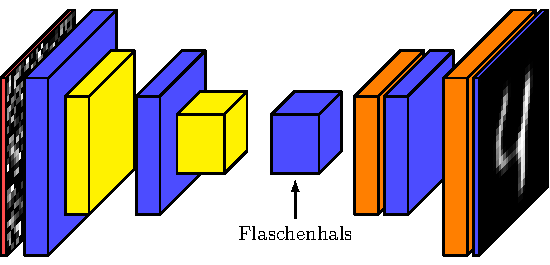
\includegraphics[width=0.7\textwidth]{themodel.pdf}
  \caption{Schema des beschriebenen Modells (Tensoren sind nicht massstabsgetreu)}
  \label{fig:the_model}
\end{figure}

\subsection{Daten}
Als Trainingsdaten wird der \keyword{MNIST}-Datensatz verwendet. Es handelt sich
dabei um den wohl bekannteste Datensatz für beispielhaftes Maschinelles Lernen.
Er besteht aus schwarz-weiss Bildern von handgeschriebenen Ziffern.
Der Datensatz würde eigentlich auch Labels zu den Ziffern enthalten, um das Modell beispielsweise
für Ziffernerkennung trainieren zu können. Jedoch ist dies hier nicht notwendig,
weil ein Autoencoder entwickelt werden soll, dessen Labels den Inputs entsprechen.
\para{}
Der Datensatz besteht aus einem Trainingsdatensatz von 60'000 Samples und einem Testdatensatz
von 10'000 Samples. Alle Ziffern sind bereits korrekt formatiert, da ihre Grösse
auf $28 \times 28$ Pixel normalisiert wurde und sie im Bild zentriert sind. Ein
Auszug an MNIST-Ziffern ist in Abbildung \refbox{fig:minst} zu sehen.
\para{}
\begin{figure}[h!]
  \centering
  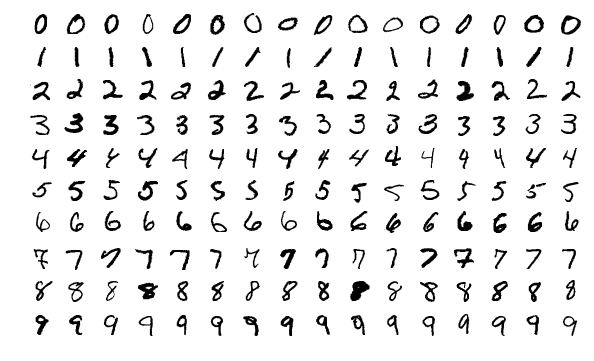
\includegraphics[width=0.6\textwidth]{mnist.png}
  \caption{ein Auszug an MNIST-Bildern (invertierte Farben) \cite{res:mnist_images}}
  \label{fig:minst}
\end{figure}
\para{}
Quellen: \cite{net:mnist}

\section{Setup}
Zunächst ist es wichtig, das Entwicklungsumfeld richtig zu konfigurieren. Das
bedeutet konkret, dass Python zusammen mit den verschiedenen Programmbibliotheken
installiert werden muss.
Die Installationsschritte werden in dieser Arbeit für eine arch-basierte
Linuxdistribution erklärt, welche den \keyword{Pacman}-Package-Manager verwendet.
Falls der Leser ein anderes Betriebssystem verwenden möchte, ist auf die offizielle
TensorFlow Website für die Installationsschritte zu verweisen (siehe QR-Code).
\para{}
\begin{minipage}{4cm}
  \centering
  \qrcode[height=2cm]{https://www.tensorflow.org/install}
  \captionof{figure}{QR-Code für Installationsanweisungen}
\end{minipage}

\paragraph{Python3}
Damit TensorFlow und Keras verwendet werden können, bedingt dies, dass Python3
installiert sein muss.
Folgender Befehl muss in der Kommandozeile ausgeführt werden, um die
Installation durchzuführen.
\begin{minted}[frame=lines,framesep=2mm,baselinestretch=1.2,bgcolor=lightgray,fontsize=\footnotesize]{bash}
  sudo pacman -S python
\end{minted}

\paragraph{TensorFlow}
Für die Installation von TensorFlow muss unter Arch Linux das entsprechende
Package installiert werden.
Falls der Leser über eine Nvidia-Grafikkarte verfügt, welche eine ``Compute
Capability'' von mehr als 3.5 besitzt, kann er von der
GPU-Hardwarebeschleunigung Gebrauch machen.
Somit ist die CUDA-Version von TF mithilfe des folgenden Kommandos zu installieren:
\begin{minted}[frame=lines,framesep=2mm,baselinestretch=1.2,bgcolor=lightgray,fontsize=\footnotesize]{bash}
  sudo pacman -S python-tensorflow-cuda
\end{minted}
Pacman installiert nun automatisch zuerst alle Programmabhängigkeiten, wie
CUDA, cuDNN und das TensorFlow-Backend, bevor das eigentliche
Python-TensorFlow installiert wird.
\para{}
Falls keine geeignete Grafikkarte vorliegt, ist es ebenso möglich, die normale
TF-Version ohne Unterstützung für die GPU zu verwenden.
Dies kann durch nachstehendes Kommando vorgenommen werden:
\begin{minted}[frame=lines,framesep=2mm,baselinestretch=1.2,bgcolor=lightgray,fontsize=\footnotesize]{bash}
  sudo pacman -S python-tensorflow
\end{minted}
\para{}
Dabei muss Keras nicht explizit installiert werden, da es bereits in TensorFlow implementiert ist.

\paragraph{Python-Module}

Für das Python-Programm werden zwei Packages benötigt, welche
nicht in der Standardbibliothek von Python enthalten sind:
\begin{itemize}
\item{NumPy: Ein Package, welches verschiedene mathematische Konzepte
    implementiert; vor allem Vektor- und Matrix-Arithmetik.}
\item{Matplotlib: Ein Package zum Erstellen von Plots und Grafiken.}
\end{itemize}

Man installiert beide mit folgenden Kommandos:
\begin{minted}[frame=lines,framesep=2mm,baselinestretch=1.2,bgcolor=lightgray,fontsize=\footnotesize]{bash}
  sudo pacman -S python-numpy
  sudo pacman -S python-matplotlib
\end{minted}

\section{Entwicklung}
Nun kann die eigentliche Programmierung beginnen.

\subsection{Testprogramm}
Zunächst wird ein kleines Testprogramm geschrieben, welches überprüft, ob
alle Programmabhängigkeiten korrekt installiert sind und verwendet werden können.
In den ersten Zeilen des Pythonprogamms werden die Importstatements
geschrieben, um NumPy, Matplotlib und TensorFlow verfügbar zu machen.
Keras muss wie gesagt nicht explizit geladen werden, da es in TensorFlow
enthalten ist.
Nun können die Versionsnummern der verschiedenen Programmbibliotheken
in die Konsole geschrieben werden, um zu überprüfen, ob alles richtig konfiguriert ist.
\begin{minted}[frame=lines,framesep=2mm,baselinestretch=1.2,bgcolor=lightgray,fontsize=\footnotesize,linenos]{python}
  import numpy as np # NumPy wird impotiert
  import matplotlib as mpl # Matplotlib wird impotiert
  import tensorflow as tf # TensorFlow wird impotiert

  print(np.__version__) # Schreibt die NumPy-Version nach stdout.
  print(mpl.__version__) # Schreibt die Matplotlib-Version nach stdout.
  print(tf.__version__) # Schreibt die TensorFlow-Version nach stdout.
\end{minted}
Falls der Output folgenden Charakter hat (die Versionsnummern müssen nicht
die gleichen sein) und keine Fehlermeldungen erfolgen, sollte alles funktionieren.
\begin{minted}[frame=lines,framesep=2mm,baselinestretch=1.2,bgcolor=lightgray,fontsize=\footnotesize,linenos]{text}
  1.17.0
  3.1.1
  1.14.0
\end{minted}
\para{}

\subsection{Trainingsdaten}
Nun wurde mit dem kleinen Testprogramm verifiziert, dass alle
Programmabhängigkeiten funktionieren. Auf dieser Basis können wir mit dem
eigentlichen Programm beginnen.
\para{}
In den folgenden Ausschnitten wird der Code laufend weiter ausgebaut.
Auf diese Weise zeigt sich, was er bewirkt.
Das eigentliche Programm startet mit folgenden Importstatements:
\begin{minted}[frame=lines,framesep=2mm,baselinestretch=1.2,bgcolor=lightgray,fontsize=\footnotesize,linenos]{python}
  import numpy as np
  import matplotlib.pyplot as plt
  import tensorflow as tf
\end{minted}

\subsubsection{Laden des MNIST-Datensatzes}
Der erste Schritt besteht darin, die Datensätze zu laden. Wie bereits
erwähnt, wird dabei vom MNIST-Datensatz Gebrauch gemacht. Da dieser stark verbreitet ist,
existiert eine Funktion in Keras, welche automatisch diese Daten herunterlädt
und sie als NumPy-Arrays zur Verfügung stellt.
Die Funktion gibt die verschiedenen Komponenten der Daten in folgendem Format zurück \code{(x\_train, y\_train),
  (x\_test, y\_test)}.
Da nur Interesse an den Features \code{x} besteht, werden die überflüssigen
Labels \code{y} mithilfe der Wegwerf-Variable \code{\_} verworfen.
\begin{minted}[frame=lines,framesep=2mm,baselinestretch=1.2,bgcolor=lightgray,fontsize=\footnotesize,linenos]{python}
  (x_train, _), (x_test, _) = tf.keras.datasets.mnist.load_data()
\end{minted}
Nun sind die Features für das Training in der Variable \code{x\_train} und die
Features des Trainingsdatensatzes in der Variable \code{x\_test} gespeichert.

\subsubsection{Formatieren der Daten}
In einem nächsten Schritt müssen die Daten transformiert werden, damit sie die
richtige Form für das Modell aufweisen.
Wie bereits erwähnt, ist der MNIST-Datensatz unkompliziert verwendbar,
da alle Bilder die gleichen Masse aufweisen und die Ziffern zentriert sind.
\para{}
Jedoch sind die Grauwerte zu normalisieren, denn im Moment liegen sie noch im
Intervall $[0, 255]$ und sind vom Typ Integer.
Das Modell kann am besten mit Kommazahlen, welche im Intervall $[0,1]$ liegen,
umgehen. Um diese Anpassung vorzunehmen, kann folgender Code angefügt werden:
\begin{minted}[frame=lines,framesep=2mm,baselinestretch=1.2,bgcolor=lightgray,fontsize=\footnotesize,linenos]{python}
  x_train = x_train.astype('float32') / 255.0 # Normalisierung
  x_test = x_test.astype('float32') / 255.0 # Normalisierung
\end{minted}
Des Weiteren werden im Modell Conv2D-Schichten verwendet. Diese in Keras
implementierten Conv2D-Schichten erwarten Inputs in der Form $(m, w, h, c)$, wobei
$m$ die Anzahl der Bilder ist, $w$ die Bildbreite, $h$ die Bildhöhe und $c$ die
Anzahl der Farbkomponenten. Die Bildbreite $w$ und -höhe $h$ von 28 Pixeln wird beibehalten, wie auch
die Anzahl Farbkomponenten $c=1$. Die Anzahl Bilder $m$ lässt sich aus der Länge
des Arrays entnehmen \code{len(x\_train)}. Mithilfe vom NumPy lässt sich das Array wie folgt umformen.
\begin{minted}[frame=lines,framesep=2mm,baselinestretch=1.2,bgcolor=lightgray,fontsize=\footnotesize,linenos]{python}
  x_test = np.reshape(x_test, (len(x_test), 28, 28, 1)) # neue Form: (60'000, 28, 28, 1)
  x_train = np.reshape(x_train, (len(x_train), 28, 28, 1)) # neue Form: (10'000, 28, 28, 1)
\end{minted}
Die Daten besitzen nun die richtige Form für das Modell.

\subsubsection{Generieren der verrauschten Bilder}\label{sec:generierung_verrauschte_bilder}
Als Input für das Modell werden nicht die normalen MNIST-Bilder verwendet, sondern
eine verrauschte Variante von diesen. Sie werden generiert, indem ein
additives Gauss'sches Rauschen auf sie angewendet wird.
\para{}
Zuerst wird eine Matrix $\mat{R} \in \set{R}^{28 \times 28 \times 1}$ erstellt, welche die gleiche Form wie die
Bilder besitzt. Diese Matrix wird mit Zufallswerten gefüllt. Für die
Zufallswerte wird eine normalisierte Gauss'sche Normalverteilung
$\mathcal{N}(\mu = 0, \sigma^2 = 1)$ mit Erwartungswert $\mu = 0$ und Varianz
$\sigma^2 = 1$ verwendet. Da jedes Bild eine eigene Rauschmatrix verlangt,
wird zu diesem Zweck eine Liste $(\mat{R}_1,\mat{R}_2,\ldots,\mat{R}_m$) der Länge $m$ an
Rauschmatrizen erzeugt. Dafür kann die NumPy Funktion
\code{np.random.normal(loc=<$\mu$>, scale=<$\sigma^2$>,size=<Form>)} verwendet werden.
Die somit erhaltenen Rauschmatrizen werden dann mit einer Rauschkonstante
\code{noise\_factor} multipliziert und anschliessend wird das Produkt auf die
MNIST-Bilder addiert. Vorerst wird der $\code{noise\_factor} = 0.5$ gewählt.
Nach dem Hinzufügen der Rauschwerte müssen die Grauwerte noch auf das Intervall
$[0,1]$ zurecht gestutzt werden. Auch hierfür kann eine NumPy-Funktion
\code{np.clip(var, min, max)} angewendet werden. Diese Schritte werden sowohl mit dem
Trainingsdatensatz, als auch mit dem Testdatensatz vollzogen. \\
Somit lautet der Code:
\begin{minted}[frame=lines,framesep=2mm,baselinestretch=1.2,bgcolor=lightgray,fontsize=\footnotesize,linenos]{python}
  noise_factor = 0.5

  # für x_train
  noise_matrices = np.random.normal(loc=0.0, scale=1.0, size=x_train.shape)
  noise_matrices *= noise_factor
  x_train_noisy = x_train + noise_matrices
  x_train_noisy = np.clip(x_train_noisy, 0.0, 1.0)

  # für x_test in Kurzfassung
  x_test_noisy = x_test + noise_factor * np.random.normal(loc=0.0, scale=1.0, size=x_test.shape)
  x_test_noisy = np.clip(x_test_noisy, 0.0, 1.0)
\end{minted}
\para{}
Mithilfe der Matplotlib kann ein Blick auf die verrauschten Bilder im Vergleich zu
den Originalbildern geworfen werden.
Dafür wird ein Plot erstellt, welcher jeweils 10 Bilder beider Arrays zeigt.
\para{}
Für diesen Zweck wird eine \code{pyplot.figure} erstellt. Innerhalb dieser
werden jeweils 10 \code{subplots} definiert, sowohl für die verrauschten Bilder, als
auch für die Originale.
Bevor die Bilder angezeigt werden können, müssen sie in die richtige Form für
die Matplotlib gebracht werden. Sie sollen die Form $(28 \times 28)$ aufweisen.
Ausserdem ist der Plot als schwarz-weiss Grafik zu spezifizieren.
\begin{minted}[frame=lines,framesep=2mm,baselinestretch=1.2,bgcolor=lightgray,fontsize=\footnotesize,linenos]{python}
  n = 10 # jeweils 10 Bilder
  plt.figure()
  for i in range(n):
    # Originalbilder
    ax = plt.subplot(2, n, 1+i)
    img_clean = x_test[i].reshape(28, 28)
    plt.imshow(img_clean)
    plt.gray()

    # verrauschte Bilder
    ax = plt.subplot(2, n, 1+n+i)
    img_noisy = x_test_noisy[i].reshape(28, 28)
    plt.imshow(img_noisy)
    plt.gray()
  plt.show()
\end{minted}

Das Ergebnis ist in Abbildung \refbox{fig:noisy_clean_mnist} sichtbar.
\begin{figure}[h!]
  \centering
  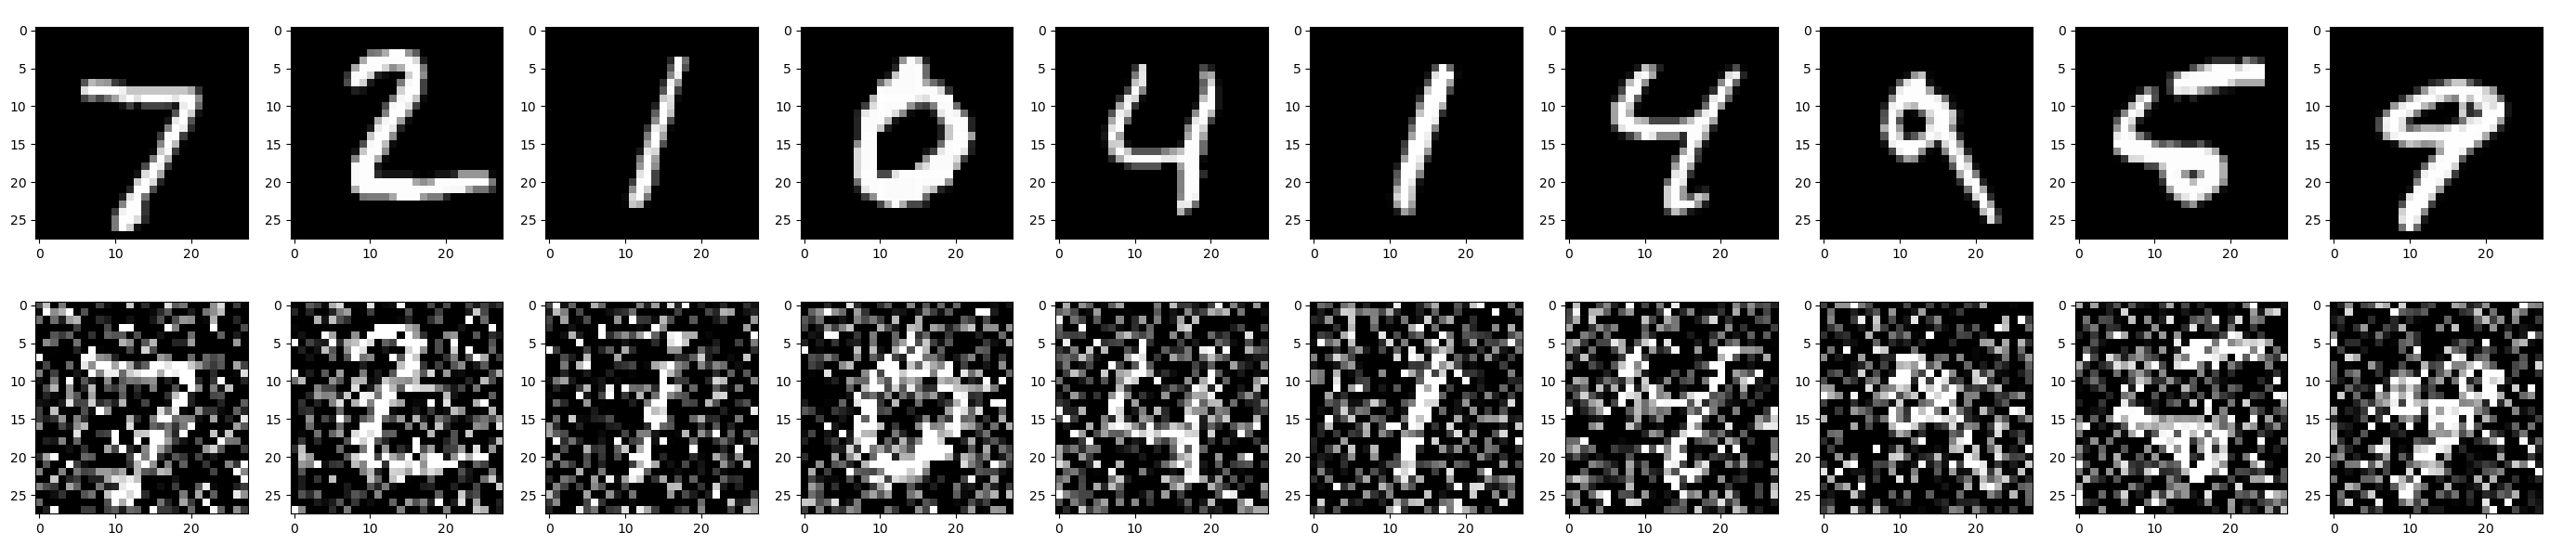
\includegraphics[width=0.9\textwidth]{noised.png}
  \caption{Verrauschte Bilder neben den Orignalbildern}
  \label{fig:noisy_clean_mnist}
\end{figure}
\para{}
Die Daten liegen nun vollständig und im richtigen Format vor.
Nun kann zur Definition des Modells übergegangen werden.

\subsection{Modell definieren}
Mithilfe von Keras kann das Modell eines Convolutional-Denoising-Autoencoder
definiert werden. Dies geschieht nach dem Vorbild der Theorie.
Wie bereits erklärt umfasst die Topologie eines CNNs die verschiedensten Hyperparameter.
Für diese werden der Einfachheit halber zunächst willkürliche Werte verwendet.
Zu einem späteren Zeitpunkt werden die passenden Hyperparameter durch iteratives Ausprobieren ermittelt.
\para{}
Das Modell beginnt mit der Inputschicht $l=0$, welche ein Tensor ist, der
die Inputwerte enthält. Die Schicht hat logischerweise die gleiche Form, wie ein MNIST-Bild.
\begin{minted}[frame=lines,framesep=2mm,baselinestretch=1.2,bgcolor=lightgray,fontsize=\footnotesize,linenos]{python}
  input_data = tf.keras.Input(shape=(28, 28, 1))
\end{minted}
\para{}
Nach dieser Inputschicht folgt der Encoder des Autoencoders. Dieser besteht
sowohl aus Convolutional-Schichten, wie auch aus Pooling-Schichten, welche sich abwechseln.
Für alle Schichten werden vorerst unbegründete Hyperparameter gewählt.
Für die Convolutional-Schichten wird
eine Filtergrösse $f^l = 3$, eine Anzahl Filter von $c^l = 32$,
ein Stride $s^l=1$, Same-Padding und die ReLU-Aktivierungsfunktion $\varphi =
\varphi^{\text{ReLU}}$ verwendet.
Da Keras standardmässig die Initialisierung der Modellparameter mit einer
uniformen Verteilung vornimmt, muss der \code{kernel\_initalizer} explizit auf
\code{'glorot\_normal'} gesetzt werden. Dadurch findet die Initialisierung analog
zu Sektion \refbox{sec:parameter_initialisieren} statt. \\
Der Code für die Definition einer solchen Convolutional-Schicht lautet:
\begin{minted}[frame=lines,framesep=2mm,baselinestretch=1.2,bgcolor=lightgray,fontsize=\footnotesize,linenos]{python}
  conv_layer = tf.keras.layers.Conv2D(filters=32, kernel_size=(3, 3),
  strides=(1, 1), padding='same', activation='relu',
  kernel_initializer='glorot_normal')
\end{minted}
Für die Pooling-Schichten wird analog eine Feldgrösse $f = 2$, ein
Stride $s = 2$ und Same-Padding gewählt. Dies bewirkt, dass jedes $(2
\times 2)$-Feld zu einem einzigen Element zusammengefasst wird. \\
Der Code für eine dieser Pooling-Schichten lautet:
\begin{minted}[frame=lines,framesep=2mm,baselinestretch=1.2,bgcolor=lightgray,fontsize=\footnotesize,linenos]{python}
  pool_layer = tf.keras.layers.MaxPooling2D(pool_size=(2, 2), strides=None, padding='same')
\end{minted}
Für den Decoder werden die gleichen Convolutional-Schichten wie für den Encoder
verwendet. Anstelle von Pooling-Schichten verwendet er UpSampling-Schichten,
welche jeweils nach einer Convolutional-Schicht folgen.
Für die UpSampling-Schichten wurde eine Feldgrösse $f = 2$ gewählt. Somit wird
ein einziger Pixel auf ein $(2 \times 2)$-Felder hochskaliert.
Als Interpolationsmethode wird der Nächste-Nachbar-Algorithmus verwendet.
Die beschriebene UpSampling-Schicht wird folgendermassen definiert:
\begin{minted}[frame=lines,framesep=2mm,baselinestretch=1.2,bgcolor=lightgray,fontsize=\footnotesize,linenos]{python}
  upsampling_layer = tf.keras.layers.UpSampling2D(size=(2, 2), interpolation='nearest')
\end{minted}
Nun folgt die Deklarierung aller Schichten und deren Verknüpfung. \\
Das Modell weist einen Flaschenhals auf, welcher zwei Convolutional-Schichten
tief ist. Das bedeutet, dass der Encoder aus zwei
Conv-Pool-Paaren besteht. Danach folgt der einschichtige
Flaschenhals. Im Anschluss daran folgt der Decoder, der zwei
Conv-UpSampling-Paare umfasst.
Um die jeweils neue Schicht zur vorherigen Schicht zu verbinden, gibt man die
vorherige in Klammern am Ende des Statements an. \\
Der ganze Graph wird durch folgenden Code gebildet:
\begin{minted}[frame=lines,framesep=2mm,baselinestretch=1.2,bgcolor=lightgray,fontsize=\footnotesize,linenos]{python}
  # Encoder
  input_data = tf.keras.Input(shape=(28, 28, 1))
  econv0 = tf.keras.layers.Conv2D(filters=32, kernel_size=(3, 3), strides=(1, 1), padding='same',
    activation='relu', kernel_initializer='glorot_normal')(input_data)
  emaxpool0 = tf.keras.layers.MaxPooling2D(pool_size=(2, 2), strides=None, padding='same')(econv0)
  econv1 = tf.keras.layers.Conv2D(filters=32, kernel_size=(3, 3), strides=(1, 1), padding='same',
    activation='relu', kernel_initializer='glorot_normal')(emaxpool0)
  emaxpool1 = tf.keras.layers.MaxPooling2D(pool_size=(2, 2), strides=None, padding='same')(econv1)

  # Flaschenhals der Form (7, 7, 32)
  encoded =  emaxpool1

  # Decoder
  dconv0 = tf.keras.layers.Conv2D(filters=32, kernel_size=(3, 3), strides=(1, 1), padding='same',
    activation='relu', kernel_initializer='glorot_normal')(encoded)
  dupsample0 = tf.keras.layers.UpSampling2D(size=(2, 2), interpolation='nearest')(dconv0)
  dconv1 = tf.keras.layers.Conv2D(filters=32, kernel_size=(3, 3), strides=(1, 1), padding='same',
    activation='relu', kernel_initializer='glorot_normal')(dupsample0)
  dupsample1 = tf.keras.layers.UpSampling2D(size=(2, 2), interpolation='nearest')(dconv1)
  dconv2 = tf.keras.layers.Conv2D(filters=1, kernel_size=(3, 3), strides=(1, 1), padding='same',
    activation='sigmoid', kernel_initializer='glorot_normal')(dupsample1)
  decoded = dconv2
\end{minted}
Auffallend im Code ist, dass der Decoder nicht etwa zwei Convolutional-Layers
besitzt, sondern sogar drei. Die letzte Schicht wird benötigt, damit
die Daten wieder die richtige Formatierung aufweisen. Das heisst einerseits,
dass die Outputs wieder in der Ursprungsform $(28 \times 28)$ vorliegen müssen.
Andererseits sollen sich die Outputs wieder im Intervall
$[0,1]$ befinden. Mithilfe der Sigmoid-Aktivierungsfunktion $\varphi^{\text{sig}}$ werden
sie genau auf dieses Intervall abgebildet.
Für alle anderen Schichten wurde die ReLU-Aktivierungsfunktion gewählt.
\para{}
Nun muss noch eine Modellvariable deklariert werden. Als Argumente erwartet
diese die Inputschicht \code{input\_data} und die Outputschicht \code{decoded}.
Danach ist das Modell zu kompilieren. Bei der Kompilierung kann das
Optimierungsverfahren und die Kostenfunktion gewählt werden. Für die Optimierung
wird das Stochastische-Gradientenverfahren SGD verwendet.
Als Kostenfunktion wird der Mittlere-Quadratische-Fehler $C_{\text{MSE}}$ gewählt.
\begin{minted}[frame=lines,framesep=2mm,baselinestretch=1.2,bgcolor=lightgray,fontsize=\footnotesize,linenos]{python}
  autoencoder = tf.keras.Model(input_data, decoded)
  autoencoder.compile(optimizer='sgd', loss='mean_squared_error') # SGD und MSE
\end{minted}
Mithilfe von \code{tf.keras.Model.summary} kann man eine Zusammenfassung des
Modells in Textform erhalten. So können Informationen bezüglich der Form der
verschiedenen Schichten abgerufen werden, um zu überprüfen, ob alles stimmig ist.
Nachfolgende Summary gilt für unser Modell:
\begin{minted}[frame=lines,framesep=2mm,baselinestretch=1.2,bgcolor=lightgray,fontsize=\footnotesize,linenos]{text}
  _________________________________________________________________
  Layer (type)                 Output Shape              Param #
  =================================================================
  input_1 (InputLayer)         [(None, 28, 28, 1)]       0
  _________________________________________________________________
  conv2d (Conv2D)              (None, 28, 28, 32)        320
  _________________________________________________________________
  max_pooling2d (MaxPooling2D) (None, 14, 14, 32)        0
  _________________________________________________________________
  conv2d_1 (Conv2D)            (None, 14, 14, 32)        9248
  _________________________________________________________________
  max_pooling2d_1 (MaxPooling2 (None, 7, 7, 32)          0
  _________________________________________________________________
  conv2d_2 (Conv2D)            (None, 7, 7, 32)          9248
  _________________________________________________________________
  up_sampling2d (UpSampling2D) (None, 14, 14, 32)        0
  _________________________________________________________________
  conv2d_3 (Conv2D)            (None, 14, 14, 32)        9248
  _________________________________________________________________
  up_sampling2d_1 (UpSampling2 (None, 28, 28, 32)        0
  _________________________________________________________________
  conv2d_4 (Conv2D)            (None, 28, 28, 1)         289
  =================================================================
  Total params: 28,353
  Trainable params: 28,353
  Non-trainable params: 0
  _________________________________________________________________
\end{minted}
Es zeigt sich, dass das Modell gesamthaft circa 28'000 Parameter umfasst,
welche zu trainieren sind.
\para{}
Quelle: \cite{net:keras_tut}

\subsection{Modell trainieren}
Das definierte Modell ist nun zu trainieren.
Mit Keras kann dies durch einen einzigen Funktionsaufruf erfolgen.
Diese Funktion erwartet einige Argumente. Zuerst sind die Features und Labels anzugeben. Die
Features wurden in der Variable \code{x\_train\_noisy} gespeichert. Die Labels
sind die unverrauschten MNIST-Bilder, welche in der Variable \code{x\_train} enthalten sind.
Des Weiteren wird die Grösse eines Mini-Batches als 128 Samples spezifiziert. Das
Training erfolgt über 100 Epochen.
Wichtig ist, dass die Trainingssamples vor dem Training durchmischt werden,
damit das Modell nicht versucht, Muster innerhalb der Anordnung der Samples zu
erlernen. Als letztes Argument wird noch der Testdatensatz angegeben.
\begin{minted}[frame=lines,framesep=2mm,baselinestretch=1.2,bgcolor=lightgray,fontsize=\footnotesize,linenos]{python}
  autoencoder.fit(x=x_train_noisy, y=x_train, batch_size=128, epochs=100, shuffle=True,
    validation_data=(x_test_noisy, x_test))
\end{minted}
Sofern TensorFlow eine geeignete Nvidia-Grafikkarte vorfindet und auch die
CUDA-Version von TF installiert ist, erfolgt das Training mithilfe von GPU-Hardwarebeschleunigung.
Dadurch sollte das Trainings innerhalb einiger Minuten abgeschlossen sein.
Während des Trainings schreibt TensorFlow Informationen zum aktuellen Fortschritt in die
Kommandozeile. Diese Informationen weisen nachstehenden Charakter auf und geben
Auskunft über die aktuelle Epoche sowie die Werte der Kostenfunktion. Die Kosten
für den Trainingsdatensatz werden mit \code{loss} bezeichnet und die für den
Testdatensatz mit \code{val\_loss}.

\begin{minted}[frame=lines,framesep=2mm,baselinestretch=1.2,bgcolor=lightgray,fontsize=\footnotesize,linenos]{text}
  Epoch 3/100
  60000/60000 [==============================] - 4s 60us/sample - loss: 0.0911 - val_loss: 0.0772
\end{minted}
Die Kostenfunktion weist nach dem Training in Bezug auf den Testdatensatz einen Wert \code{val\_los} von $0.0180$,
auf.
\para{}
Jetzt, da das Modell trainiert wurde, ist es sinnvoll, es auf dem Computer als
Modelldatei abzuspeichern. So muss es nicht jedes Mal wieder neu trainiert werden, sondern kann über
die Modelldatei eingelesen werden.
\begin{minted}[frame=lines,framesep=2mm,baselinestretch=1.2,bgcolor=lightgray,fontsize=\footnotesize,linenos]{python}
  autoencoder.save('denoiser.model')
\end{minted}
Für dieses Einlesen wird folgender Code benötigt:
\begin{minted}[frame=lines,framesep=2mm,baselinestretch=1.2,bgcolor=lightgray,fontsize=\footnotesize,linenos]{python}
  autoencoder = tf.keras.models.load_model('denoiser.model')
\end{minted}
Mit der Summary-Funktion kann man überprüfen, ob das richtige Modell geladen wurde.

\subsection{Modell ausführen}
Da das Modell nun trainiert ist, kann es für seinen eigentlichen Zweck
genutzt werden.
Dieser besteht darin, Bilder zu entrauschen. Dafür gelangen die
Bilder aus dem Testdatensatz zur Anwendung. Auf diese Weise wird garantiert, dass diese
unbenutzten Daten vom Modell nicht auswendig gelernt werden konnten.
Mit der Funktion \code{tf.keras.model.predict}
erhält man alle Vorhersagen des Autoencoders zum gesamten Testdatensatz.
\begin{minted}[frame=lines,framesep=2mm,baselinestretch=1.2,bgcolor=lightgray,fontsize=\footnotesize,linenos]{python}
  denoised_imgs = autoencoder.predict(x_test)
\end{minted}
Mithilfe von der Matplotlib können die entrauschten Bilder mit den
ursprünglichen MNIST-Bilder direkt verglichen werden.
So kann mit blossem Auge beurteilt werden, wie gut die Ergebnisse des Modells tatsächlich sind.
\begin{minted}[frame=lines,framesep=2mm,baselinestretch=1.2,bgcolor=lightgray,fontsize=\footnotesize,linenos]{python}
  n = 10 # jeweils 10 Bilder
  plt.figure()
  for i in range(n):
    # verrauschte Bilder
    ax = plt.subplot(3, n, 1+i)
    plt.imshow(x_test_noisy[i].reshape(28, 28))
    plt.gray()

    # entrauschte Bilder
    ax = plt.subplot(3, n, 1+n+i)
    plt.imshow(decoded_imgs[i].reshape(28, 28))
    plt.gray()

    # Original-Bilder
    ax = plt.subplot(3, n, 1+2*n+i)
    plt.imshow(x_test[i].reshape(28, 28))
    plt.gray()
  plt.show()
\end{minted}
In der ersten Zeile der Grafik sind die verrauschten Bilder dargestellt.
Darunter folgen die Rekonstruktionen als Ergebnis des Modells und in der dritten Zeile
sind die Original-Bilder zu sehen.
Wirkliche Unterschiede zwischen der zweiten und der dritten Zeile sind kaum zu erkennen.
\begin{figure}[h!]
  \centering
  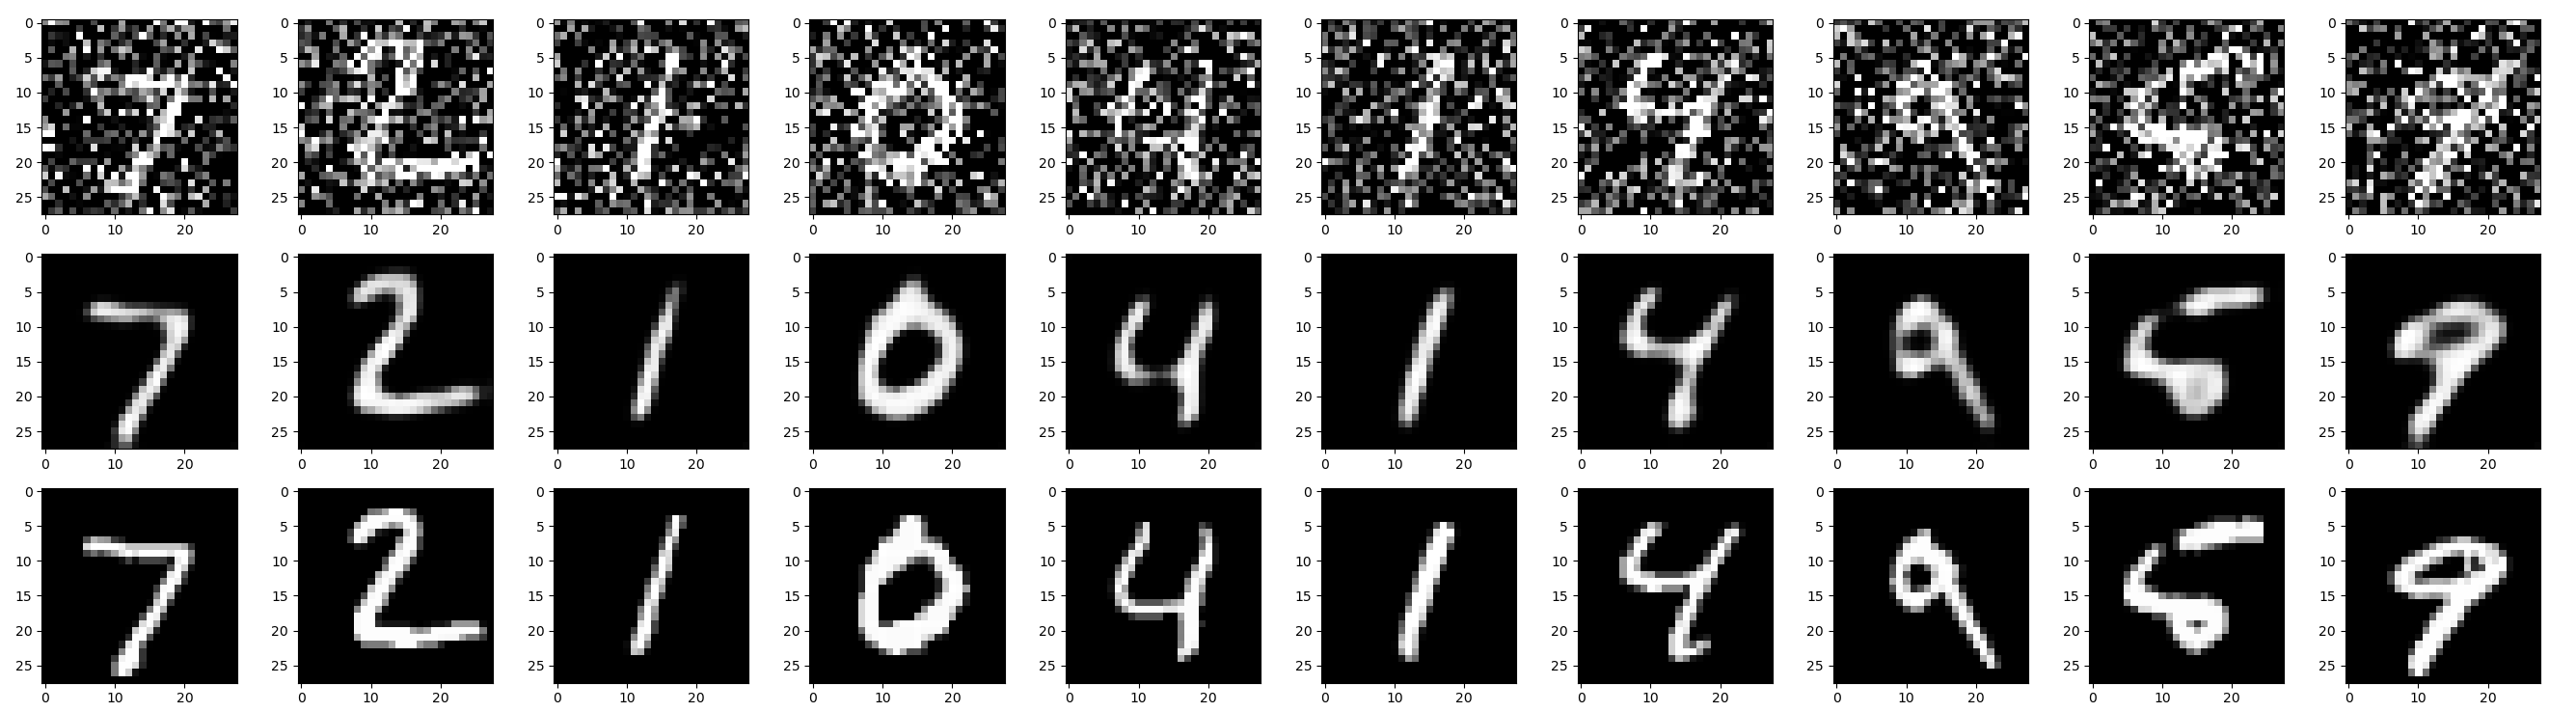
\includegraphics[width=0.9\textwidth]{denoised.png}
  \caption{Verrauschte Bilder, Rekonstruktionen und Orignalbilder}
\end{figure}

\subsection{Hyperparameter einstellen}
Für die Hyperparameter haben wir zunächst willkürliche Werte verwendet. Es
sollen nun besser geeignete Hyperparameter bestimmt werden. Dazu müssen
lediglich verschiedene Werte iterativ ausprobiert werden.
Die Applikation wird modifiziert, indem verschiedene Modelle konstruiert werden,
welche unterschiedliche Hyperparameter verwenden.
Beim Training werden mithilfe von TensorBoard
Daten zum Lernfortschritt und den Kosten der verschiedenen Modelle erfasst. Auf
diese Weise kann eine Auswertung erstellt werden, um die besten Hyperparameter
zu identifizieren.
\para{}
Zuerst werden einige Arrays definiert, welche die zu testenden Hyperparameter beinhalten.
Ein Hyperparameter ist die Anzahl Epochen. Für diesen werden wir aber nicht
verschiedene Werte ausprobieren, da es offensichtlich ist, dass sich mit einer längeren Trainingszeit auch die
Resultate verbessern.
Alle Modelle werden für 20 Epochen trainiert.
\para{}
Folgende Mini-Batch-Grössen sollen geprüft werden: 16, 32, 64, 128, 265.
Als zu testende Anzahl von Filtern werden definiert: 16, 32, 64, 128, 256.
Für die Aktivierungsfunktionen werden Sigmoid und ReLU ausprobiert. Anstatt dass
jede Schicht eine eigene Aktivierungsfunktion erhält, gelangt für das gesamte
Modell eine einzige Funktion zur Anwendung. Auf diese Weise soll die Anzahl an
Permutationen der Hyperparameter gering gehalten werden.
Jedoch wird für die letzte Schicht immer die
Sigmoid-Aktivierungsfunktion verwendet, damit die Outputs im Intervall $[0,1]$
liegen.

\begin{minted}[frame=lines,framesep=2mm,baselinestretch=1.2,bgcolor=lightgray,fontsize=\footnotesize,linenos]{python}
  EPOCHS = 20

  BATCH_SIZES = [ 16, 32, 64, 128, 256 ]
  FILTER_NUMS = [ 16, 32, 64, 128, 256 ]
  ACTIVATIONFUNCTIONS = [ 'sigmoid', 'relu' ]
\end{minted}
Nun werden wir den gesamten Code zum Erstellen des Graphen, zur Kompilierung und
zum Training des Modells in verschachtelte For-Loops verschieben, welche alle
Kombinationen von Hyperparametern ausprobieren.

\begin{minted}[frame=lines,framesep=2mm,baselinestretch=1.2,bgcolor=lightgray,fontsize=\footnotesize,linenos]{python}
  for activation_function in ACTIVATIONFUNCTIONS:
    for batch_size in BATCH_SIZES:
      for num_filters in FILTER_NUMS:
        # ganzer Modell-Code
\end{minted}
Nun muss der Code zur Definition des Modells so modifiziert werden, dass die
Konstanten an den entsprechenden Stellen durch die Variablen
\code{activation\_function}, \code{batch\_size} und \code{num\_filters} ersetzt
werden.

\subsubsection{TensorBoard konfigurieren}
Um den Lernprozess und die Leistungsfähigkeit des Modells zu analysieren,
soll nun TensorBoard konfiguriert werden.
Zu diesem Zweck müssen die Methoden \code{compile} und \code{fit} angepasst werden.
Zuerst müssen wir in der \code{compile} Methode die zu erfassenden Metriken
angeben. Von Interesse ist die \code{'accuracy'}.
\begin{minted}[frame=lines,framesep=2mm,baselinestretch=1.2,bgcolor=lightgray,fontsize=\footnotesize,linenos]{python}
  autoencoder.compile(optimizer='sgd', loss='mean_squared_error', metrics=['accuracy'])
\end{minted}
Nun ist eine TensorFlow-Variable zu definieren. Es ist anzugeben, wo
die erfassten Daten gespeichert werden sollen. Es ist sinnvoll, den Dateien
der einzelnen Modelle aussagekräftige Namen zu geben. Deshalb benennen wir die
Dateien in folgendem Format: ``denoiser-(Aktivierungsfunktion)-(Mini-Batch
Grösse)-batches-(Anzahl Filter)-filters''.
\begin{minted}[frame=lines,framesep=2mm,baselinestretch=1.2,bgcolor=lightgray,fontsize=\footnotesize,linenos]{python}
  NAME = 'denoiser-{}-{}-batches-{}-filters'.format(activation_function, batch_size, num_filters)
  tensorboard = tf.keras.callbacks.TensorBoard(log_dir='logs/{}'.format(NAME))
\end{minted}
Zuletzt muss noch die TensorBoard-Variable als \code{callback} in der
\code{fit}-Methode spezifiziert werden.
\begin{minted}[frame=lines,framesep=2mm,baselinestretch=1.2,bgcolor=lightgray,fontsize=\footnotesize,linenos]{python}
  autoencoder.fit(x=x_train_noisy, y=x_train, batch_size=batch_size, epochs=EPOCHS, shuffle=True,
    validation_data=(x_test_noisy,x_test), callbacks=[tensorboard])
\end{minted}
Nun kann das modifizierte Programm ausgeführt werden. Dabei werden alle
spezifizierten Kombinationen an Hyperparametern durchgetestet. Gleichzeitig
erzeugt das TensorBoard-Callback Logdateien im \code{'logs'}-Verzeichnis. Diese
Dateien enthalten alle nötigen Informationen zur anschliessenden Auswertung.

\subsubsection{TensorBoard-Analyse}
Um die besten Hyperparameter mithilfe von TensorBoard zu bestimmen, muss
zunächst der TensorBoard-Webserver gestartet werden. Dafür navigiert man
mit der Kommandozeile in das Verzeichnis, welches die Logdateien enthält.
Dort kann dann der Webserver mithilfe folgendem Kommando gestartet werden.
\begin{minted}[frame=lines,framesep=2mm,baselinestretch=1.2,bgcolor=lightgray,fontsize=\footnotesize,linenos]{text}
tensorboard --logdir .
\end{minted}
Nun kann mit einem Webbrowser zur angegebenen Webadresse navigiert werden. In
der Regel lautet diese: \code{http://localhost:6006/}.
Der Graph, welcher die Kosten bezüglich des Testdatensatzes aufzeichnet, ist von besonderem
Interesse. Dieser sieht folgendermassen aus:
\para{}
\begin{figure}[h!]
  \centering
  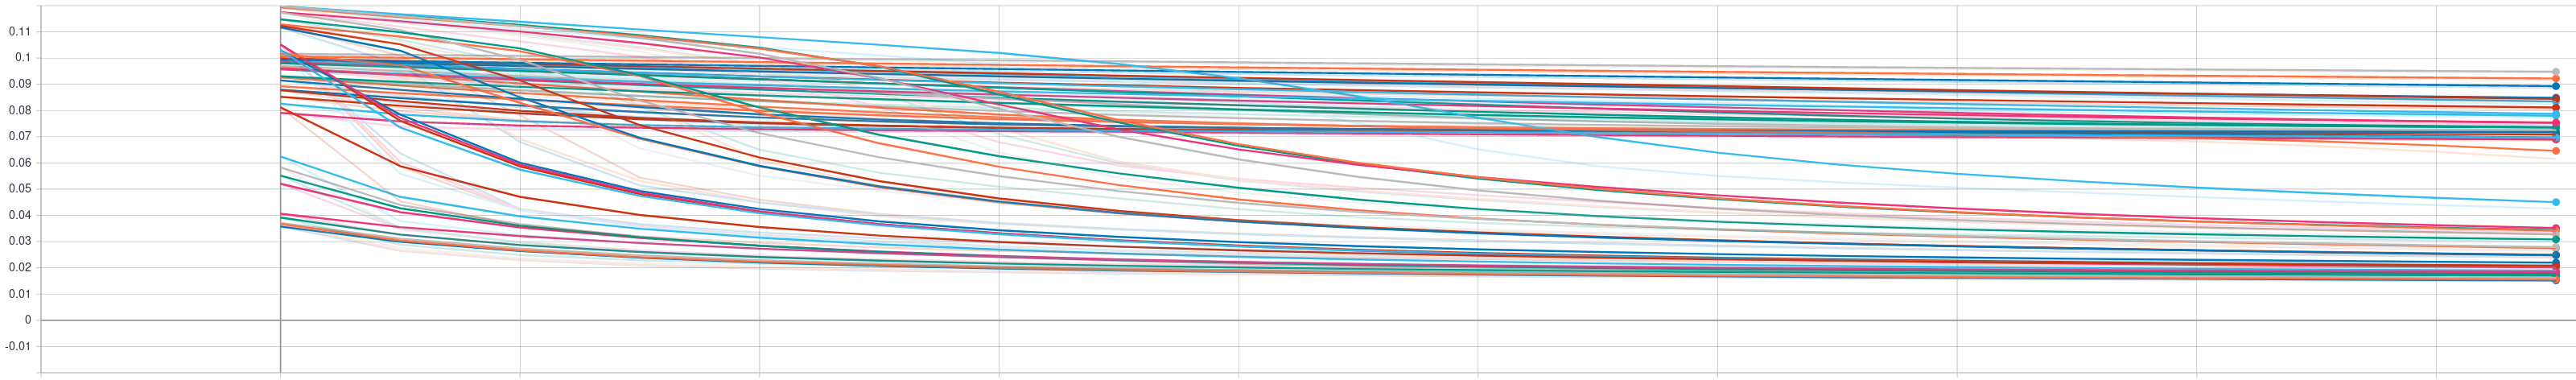
\includegraphics[width=1\textwidth]{tb_results.png}
  \caption{Kosten bezüglich dem Testdatensatz}
\end{figure}
\para{}
Dank dem interaktiven Interface von TensorBoard, kann dem Graphen entnommen
werden, welche Werte der Hyperparameter die besten Resulate liefern.

\para{}
\begin{table}[h!]
  \centering
  \begin{tabular}{ |c|c|c|c|c| }
    \hline
    Rang & Aktivierungsfunktion & Minibatch-Grösse & Anzahl Filter & Kosten \\
    \hline
    1 & ReLU & 16 & 265 & 0.015 \\
    2 & ReLU & 16 & 128 & 0.01521 \\
    3 & ReLU & 16 & 64 & 0.01588 \\
    4 & ReLU & 16 & 32 & 0.0167 \\
    $\vdots$ & $\vdots$ & $\vdots$ & $\vdots$ & $\vdots$ \\
    50 & Sigmoid & 256 & 16 & 0.09438 \\
    \hline
  \end{tabular}
  \caption{Rangliste der besten Modelle mit ihren Eigenschaften}
  \label{tab:rangliste}
\end{table}
\para{}
Die geeigneten Hyperparameter konnten jetzt identifizieren werden. Um die
Leistungsfähigkeit des Modells aufzuzeigen, wird es unter Verwendung
der gefundenen Hyperparameter nochmals zur Bildentrauschung eingesetzt.
Das diesbezügliche Training soll wiederum 100 Epochen umfassen.
Aufgrund der erwarteten höheren Leistungsfähigkeit wird in diesem Durchlauf der
\code{noise\_factor} von 0.5 (vgl. \refbox{sec:generierung_verrauschte_bilder}) auf
1 gesetzt. Das Rauschentfernen wird dadurch anspruchsvoller. Die Ergebnisse sind
in unten stehender Abbildung zu erkennen.
\begin{figure}[h!]
  \centering
  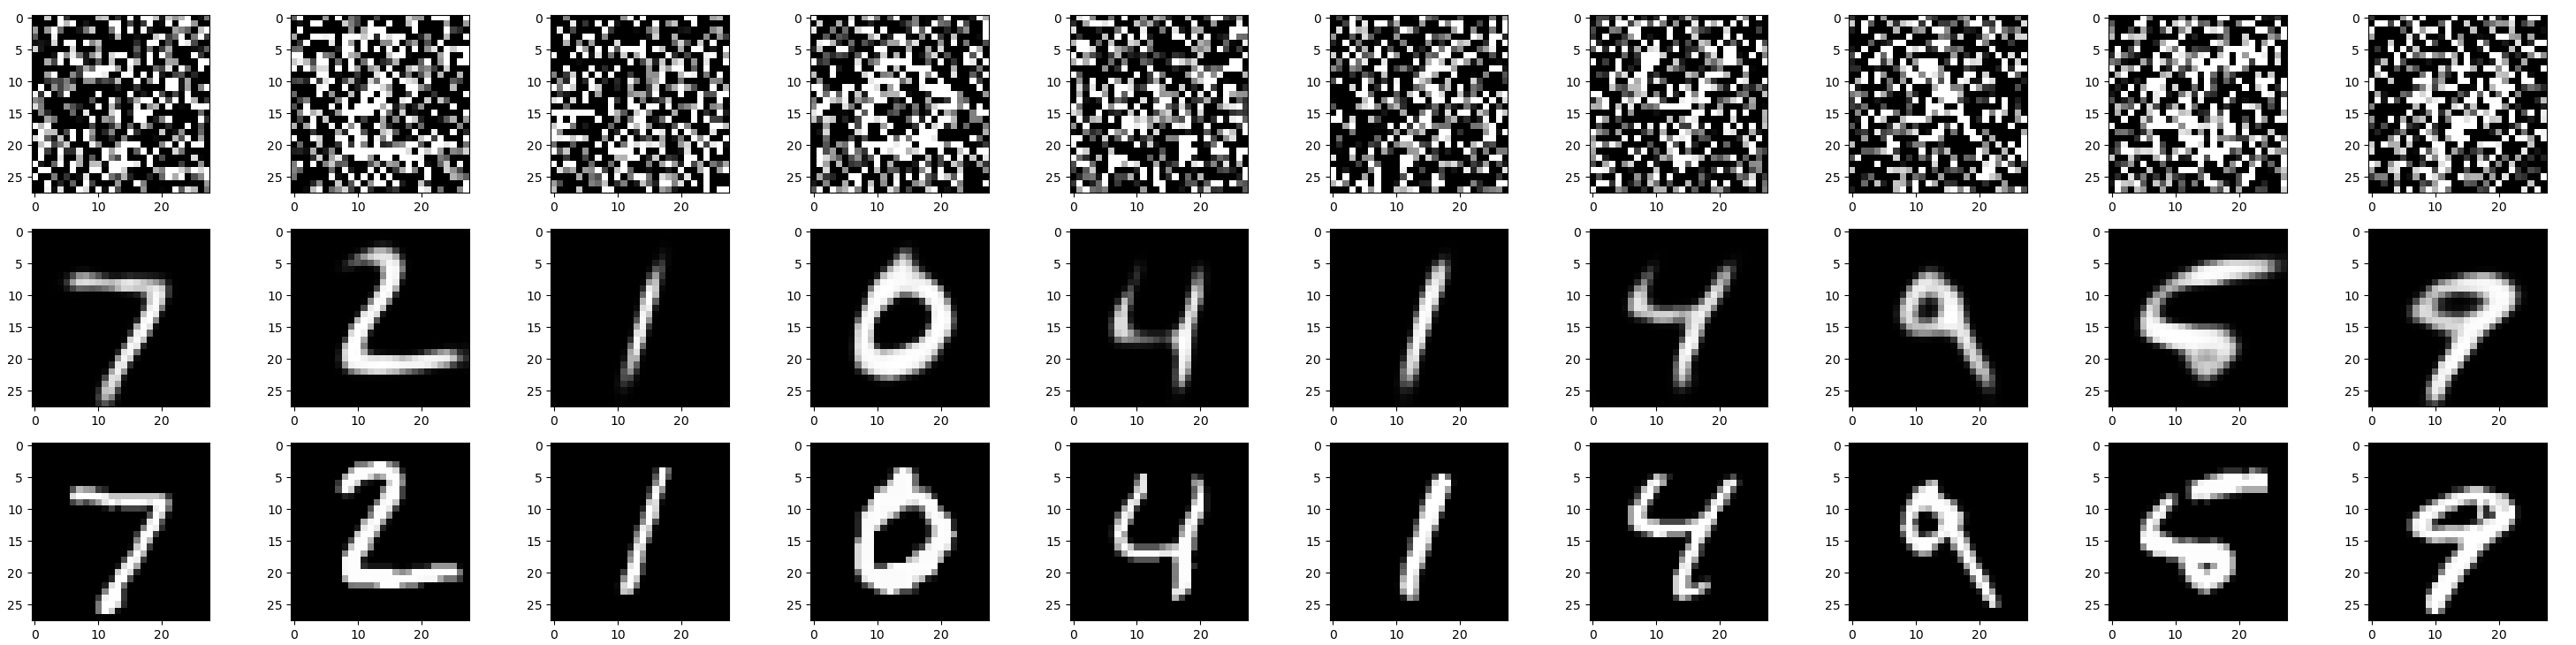
\includegraphics[width=0.9\textwidth]{denoised_best.png}
  \caption{Sehr verrauschte Bilder, Rekonstruktionen und Originalbilder}
\end{figure}


\subsection{Diskussion des Modells}
Das entwickelte Modell soll an dieser Stelle bezüglich seiner Leistungsfähigkeit
diskutiert werden.

\subsubsection{Leistung des Modells}
Die Leistung des Modells kommt am besten in der letzten Abbildung zur
Geltung. Da die Hyperparameter nun optimaler gewählt wurden, ist das Modell auch
in der Lage, extrem verrauschte Ziffern wieder gut erkennbar zu machen. Dem
menschlichen Auge fällt es schwer, noch klare Ziffern in den verrauschten Bildern
auszumachen. Das Modell hingegen kann verblüffend gut die Ziffern rekonstruieren
und gänzlich von ihrem Rauschen befreien. Dies ist für ein vergleichsweise
einfaches Programm eine bemerkenswerte Leistung.

\subsubsection{Ergebnisse der Hyperparameter}
Die Ergebnisse der Auswertung mit TensorBoard stimmen ziemlich gut mit meinen
Erwartungen überein. Wie bereits in der Theorie geäussert, liefert die
ReLU-Aktivierungsfunktion bessere Ergebnisse in CNNs als die Sigmoidfunktion.
Deshalb sind die ersten Plätze der Rangliste (vgl. Tabelle \refbox{tab:rangliste}) nur mit Modellen, welche die
ReLU-Funktion verwenden, besetzt. Weiter ist auffallend, dass die besten Modelle
möglichst tiefe Minibatch-Grössen verwenden. Dies ist naheliegend, da eine
kleine Grösse mit einer höheren Präzision der Gradientenapproximation
einhergeht. Somit ist der Gradientenabstieg exakter. Jedoch hat dies auch seine
Schattenseite: Die Motivation hinter zur Einführung der
Minibatches für SGD liegt darin, die Trainingszeit zu verkürzen. Durch die
kleineren Batches nimmt die Trainingszeit jedoch erheblich zu.
Eine weitere Feststellung ist, dass eine höhere Anzahl an Filtern das Modell zu
besseren Resultaten führt. Jedoch ist der Einfluss dieses Hyperparameters
geringer als jene der übrigen.

\subsubsection{Verbesserungsmöglichkeiten}
Es gibt konkrete Verbesserungsmöglichkeiten, welche bei der Entwicklung
des Denoisers bewusst nicht umgesetzt wurden.
Diese hätten womöglich für noch bessere Resultate gesorgt. Allerdings hätten
sie den Umfang der vorliegenden Arbeit gesprengt.
\para{}
Ein erster Ansatzpunkt hätte möglicherweise darin bestanden, mehr Werte für die
Hyperparameter auszuprobieren, anstatt nur einige wenige zu testen.
\para{}
Auch wäre es möglich gewesen, anderweitige
Hyperparamter einzubeziehen, welche im vorliegenden Modell keine
Berücksichtigung gefunden haben. So wurden beispielsweise die Topologie und die
Schichtenarten gar nicht verändert. Dies hatte den
praktischen Grund, dass die Anzahl Permutationen an Hyperparametern nochmals
stark zugenommen und sich die Trainingsdauer deutlich verlängert hätte.
Ausserdem ist es schwierig, bei einem Convolutional-Autoencoder verschiedene
Topologien automatisiert zu testen. Es muss nämlich garantiert werden, dass die
Inputschicht die gleichen Dimensionen wie die Outputschicht besitzt. Dies stellt
sich als weitere Herausforderung dar.
\para{}
Eine weitere Modifikation, welche das Modell vermutlich nochmals verbessert hätte,
wäre eine alternative Kostenfunktion gewesen. So gilt beispielsweise die
\keyword{Kreuzentropie-Kostenfunktion} als deutlich raffinierter als die MSE-Kostenfunktion.
Sie stellt eine Lösung für das sogenannte \keyword{Vanishing-Gradient-Problem}
dar. Durch dessen Behebung kommt es nicht --- wie im vorliegenden Modell --- zu einer Verlangsamung des Trainings im
Verlauf des Gradientenabstiegs.
\para{}
Weitere Verbesserungen könnten in der Wahl eines anderen
Optimierungsverfahren als SGD liegen. Beispielsweise könnte eine SGD-Variante mit
Impuls (engl.: momentum) verwendet werden. Diese Art von SGD stellt ein
Verfahren dar, welches den Gradientenabstieg weniger sprunghaft macht und damit
zielstrebiger zum Minimum führt.
\para{}
Viele dieser Modifikationen wären durch einige wenige Codeänderungen im Programm
umsetzbar. Ohne deren theoretische Behandlung sind sie jedoch nur schwer
nachvollziehbar und daher für die vorliegende Arbeit nicht von höherem Wert.


%%% Local Variables:
%%% TeX-command-extra-options: "--shell-escape"
%%% TeX-master: "../main"
%%% End:

% LocalWords:  gelabelt Unüberwachtes unsupervised Inputdaten Grossteil Vector
% LocalWords:  unüberwachtem Hauptkomponentenanalysen Adversial Networks bzw Gl
% LocalWords:  Trainingssample Inputsvektor Labelvektor Overfitting Machines eq
% LocalWords:  Trainingsdaten Testdatensatz Trainingsdatensatz gewissermassen
% LocalWords:  Hypothesenfunktion Klassifizierungsprobleme Regressionsprobleme
% LocalWords:  Regressionsmodell Regressionsproblem Modellparameter Machine sec
% LocalWords:  Hyperparameter Regressionsgerade Kostenfunktionen BEISPIELMODELL
% LocalWords:  Verlustfunktionen Verlustfunktion Label Kostenfunktion Ouputs gd
% LocalWords:  Datenrauschen Autoencoder Unüberwachten autoencoder Inputvektor
% LocalWords:  overfitting Auswendiglernen errorfunc Outputpaare Grösse ref ml
% LocalWords:  meanerrorfunc ableitungen mean squared error quadrierten descent
% LocalWords:  Gradientenverfahren Optimierungsproblem Funktionswerte anhang
% LocalWords:  Gymnasialstufe Gradientenverfahrens parameter initialisieren
% LocalWords:  Lernrate Proportionalitätsfaktor Schrittgrösse Ausserdem gross
% LocalWords:  Gradientenabstiegs schiesst Aktivierungsfunktion Neurons Neural
% LocalWords:  ausserdem Zwischenschichten folgendermassen rasterartige Network
% LocalWords:  Rückwärtspropagierung Tensoren graustufiges Invarianzen Denoiser
% LocalWords:  Dimensionalität Convolutional Autoencoders
